% ===========================================================================
% A Reproducible National Agricultural Greenhouse-Gas and Air-Pollutant Inventory
% with Mass-Conserving Geospatial Allocation for Pakistan
%
% Target journal: Environmental Modelling & Software (Elsevier)
% Document class: elsarticle, 5p layout
% ===========================================================================

\documentclass[5p,times,authoryear]{elsarticle}

% ===========================================================================
% Shared preamble for every manuscript in this repository.
%
% Papers using it:
%   paper/            agriculture inventory
%   paper_nowcast/    agricultural nowcasting
%   paper_national/   the nine-sector national inventory
%   notes/<sector>/   one data note per non-agriculture sector
%
% It exists because paper/ and paper_nowcast/ began as copies of one another
% and had already drifted five lines apart before a third manuscript existed.
% Eleven copies would drift eleven ways, and a macro that renders differently
% in two papers is the kind of defect nobody notices until proof stage.
%
% \graphicspath is deliberately NOT set here - each manuscript sets its own
% after \input{...preamble}, because figures live beside the document.
% ===========================================================================

\usepackage[utf8]{inputenc}
\usepackage[T1]{fontenc}
\usepackage{amsmath,amssymb}
\usepackage{graphicx}
\usepackage{booktabs}
\usepackage{multirow}
\usepackage{siunitx}
\usepackage[colorlinks=true,citecolor=blue,linkcolor=blue,urlcolor=blue]{hyperref}
% Document-information metadata for every PDF in the bundle (the seventh review noted
% the shipped PDFs carried none). Documents that set their own \hypersetup{pdftitle=...}
% keep it - hyperref takes the LAST setting, and this shared block runs first. Full
% tagged-PDF (tagpdf / \DocumentMetadata) is deliberately not attempted here: the
% installed LaTeX toolchain's support is not uniform across sixteen documents, and a
% half-tagged bundle is worse than an honestly untagged one; deferred deliberately.
\hypersetup{
  pdfauthor={Rehan Ahmad, Pakistan Air Quality Initiative (PAQI)},
  pdfsubject={A reproducible ten-sector national greenhouse-gas inventory
              for Pakistan},
  pdfkeywords={Pakistan, greenhouse gas inventory, IPCC 2006 Guidelines, MRV,
               reproducible research, emissions, air pollutants},
}
\usepackage{caption}
\captionsetup[table]{position=below}
\usepackage{enumitem}
\usepackage{xcolor}
\usepackage{float}
\usepackage{placeins}
\usepackage{tabularx}
\usepackage{natbib}
\usepackage{tikz}
\usetikzlibrary{arrows.meta,positioning,fit,backgrounds}

\setlength{\emergencystretch}{3em}

% Looser float placement to prevent pile-up in two-column mode.
\renewcommand{\topfraction}{0.95}
\renewcommand{\bottomfraction}{0.85}
\renewcommand{\textfraction}{0.05}
\renewcommand{\floatpagefraction}{0.85}
\setcounter{topnumber}{4}
\setcounter{bottomnumber}{3}
\setcounter{totalnumber}{6}

% ---------------------------------------------------------------------------
% Custom shorthand: in macros.tex since the ESSD re-targeting, because the national
% article compiles under the Copernicus class and cannot take this preamble (the class
% loads its own packages) but needs exactly the same macros. This file inputs it so that
% every other manuscript keeps compiling unchanged.
%
% THREE relative paths, because \input resolves against the COMPILE DIRECTORY and not
% against this file, so the depth is a property of whoever is building:
%   ../paper_common      a manuscript compiled from one level down
%   ../../paper_common   papers/<sector>/ and notes/<sector>/
%   ../../../paper_common  paper_national/versions/<v>/, since the national paper was
%                          versioned - that move is what added this third arm, and the
%                          supplement failed with "../../paper_common/macros.tex not
%                          found" until it was here
% A fourth depth needs a fourth arm, which is the cost of keeping a bare `latexmk` in a
% manuscript directory working without a TEXINPUTS set for it.
% ---------------------------------------------------------------------------
\IfFileExists{../paper_common/macros.tex}%
  {\input{../paper_common/macros}}%
  {\IfFileExists{../../paper_common/macros.tex}%
    {% ===========================================================================
% paper_common/macros.tex - the shorthand every manuscript shares.
%
% Split from preamble.tex in the ESSD re-targeting: the national article now compiles
% under the Copernicus class, which loads its own packages and forbids most of what
% preamble.tex sets (geometry-like options, a second hyperref, placeins), but it needs
% exactly the same shorthand as the sector reports. The macros therefore live here, on
% their own, and preamble.tex inputs this file so that every other manuscript keeps
% compiling unchanged. A macro that renders differently in two documents is the defect
% this file exists to prevent; define it once.
%
% Requires: siunitx (for \DeclareSIUnit and \si) - the caller loads it.
% ===========================================================================

% Gas and pollutant names.
\newcommand{\COtwo}{CO\textsubscript{2}}
\newcommand{\COe}{CO\textsubscript{2}e}
\newcommand{\CHfour}{CH\textsubscript{4}}
\newcommand{\NtwoO}{N\textsubscript{2}O}
\newcommand{\NHthree}{NH\textsubscript{3}}
\newcommand{\NOx}{NO\textsubscript{x}}
\newcommand{\SOtwo}{SO\textsubscript{2}}
\newcommand{\PM}{PM\textsubscript{2.5}}
\newcommand{\MCF}{MCF}
\newcommand{\Mt}{\text{Mt~\COe}}
\newcommand{\tCha}{\si{\tonne\per\hectare}}
\newcommand{\AFOLU}{AFOLU}
\newcommand{\GLW}{GLW\,4}
\newcommand{\EFone}{EF\textsubscript{1}}

% siunitx: allow Mt, Tg, ha, head, yr, dB
\DeclareSIUnit{\head}{head}
\DeclareSIUnit{\yr}{yr}
\DeclareSIUnit{\dB}{dB}

% A file name is the one long unbreakable token these documents are full of -
% \texttt{waste\_air\_pollutants\_2024.csv} is wider than a two-column measure and TeX prints
% it past the margin rather than breaking it. Allowing a break AFTER each escaped underscore
% costs nothing and inserts no hyphen, which matters: a hyphenated file name is a wrong file
% name. This is one line because every such name in every document is written with \_.
\let\pkinvunderscore\_
\renewcommand{\_}{\pkinvunderscore\allowbreak}
}%
    {\input{../../../paper_common/macros}}}
% Long unbreakable strings - output filenames, module paths, URLs in \texttt - do not fit a
% two-column measure and TeX prints them past the margin rather than breaking them. Nothing
% read the log, so 47 of those overruns shipped across seven documents. Emergency stretch lets
% the paragraph loosen instead, and \texttt is taught to break at the punctuation these names
% actually contain.
\emergencystretch=6em


% Generated from the current ten-fiscal-year reference release; do not hand edit.
\newcommand{\SectorRefGHG}{223}
\newcommand{\SectorRefPMfine}{54.13}
\newcommand{\SectorRefBC}{3.561}
\newcommand{\SectorRefNOx}{318}
\newcommand{\SectorRefSOtwo}{2.849}
\newcommand{\SectorRefCO}{655.2}
\newcommand{\SectorRefNMVOC}{49.85}
\newcommand{\SectorRefNHthree}{2619}
\newcommand{\SectorLatestGHG}{228.6}
\newcommand{\SectorLatestPMfine}{49.9}
\newcommand{\SectorLatestBC}{3.283}
\newcommand{\SectorLatestNOx}{318.4}
\newcommand{\SectorLatestSOtwo}{2.626}
\newcommand{\SectorLatestCO}{604.1}
\newcommand{\SectorLatestNMVOC}{45.96}
\newcommand{\SectorLatestNHthree}{2639}

\graphicspath{{figures/}}

% ---------------------------------------------------------------------------
\journal{Environmental Modelling \& Software}
% ---------------------------------------------------------------------------

\begin{document}

\begin{frontmatter}

\title{PakEmis Sector Technical Note TN01\\[4pt]
A Reproducible Agricultural Greenhouse-Gas and Air-Pollutant Inventory
for Pakistan with Mass-Conserving Spatial Allocation}

\author[paqi]{Rehan Ahmad\corref{cor1}}
\ead{rehan@pakairquality.com}

\address[paqi]{Pakistan Air Quality Initiative (PAQI), Karachi, Pakistan}

\cortext[cor1]{Corresponding author}

% --- Abstract ---
\begin{abstract}
This technical note documents the agricultural contribution to PakEmis using a common livestock, crop, fertiliser and nitrogen-flow account for greenhouse gases and air pollutants. The supported national core covers July 2015--June 2025. FY2023--24 remains the detailed reference year; earlier long calendar-year diagnostics are separate products and do not define the common fiscal period.

The reference TAN-coherent configuration produces \SI{\SectorRefGHG}{\mega\tonne} \COe{} on AR5 GWP-100, \SI{\SectorRefNHthree}{\kilo\tonne} \NHthree{}, \SI{\SectorRefNOx}{\kilo\tonne} NO$_2$-equivalent \NOx{} and \SI{\SectorRefPMfine}{\kilo\tonne} primary PM$_{2.5}$ in FY2023--24. FY2024--25 uses observed fiscal crop and nutrient controls and the consistent census-anchored livestock reconstruction. Native gas masses, pollutant masses and GWP aggregates remain separate.

Species- and stage-resolved TAN losses drive both \NHthree{} and the surviving manure pools used for \NtwoO{}. An IPCC volatilisation configuration is retained separately; it is not mixed probabilistically with the TAN reference. Conditional uncertainty replays shared herd, crop, nitrogen and applicable fate-factor draws, while management shares, factor applicability and missing sources remain distinct limitations. Direct comparison with the publicly released HTAPv3.2 monthly country tables matches exact July--June periods and records shared REAS/EDGAR inputs. The release provides national activity detail and process-matched geographic support beyond a simple clipped global inventory.

\end{abstract}

\begin{keyword}
agricultural greenhouse-gas inventory \sep air-pollutant emissions \sep ammonia \sep
hybrid IPCC Tier 1/2 \sep dasymetric mapping \sep gridded livestock \sep
mass-balance reconciliation \sep district downscaling \sep Monte-Carlo uncertainty \sep
Pakistan \sep MRV \sep transparency reporting
\end{keyword}

\end{frontmatter}

%% Generated by scripts/make_release_cover.py; says which release this documents.
% The Sector Technical Note banner (v1.0.0). Each sector manuscript is a PakEmis Sector
% Technical Note, numbered TN01-TN10 in src/pkinv/release.py (TECHNICAL_NOTES), and says
% so on its first page: it documents ONE sector module of the release named in the block
% that follows, and the national totals are stated only in the data-description article
% (the cover block below reproduces them as release identity, not as a claim of this note).
% Usage, in the document body before the release cover:  \TNBanner{TN01}
\providecommand{\TNBanner}[1]{%
  \noindent\fbox{\parbox{\dimexpr\linewidth-2\fboxsep-2\fboxrule}{%
    \textbf{PakEmis Sector Technical Note #1.} Technical documentation of one sector
    module of the PakEmis release identified below, deposited with the data as part of the
    documentation record. The national data-description article (\texttt{paper\_national/})
    is the only document that states the national totals as its own result.%
    \InputIfFileExists{../../paper_common/generated_availability_tn}{}{}%
  }}\par\medskip}

\TNBanner{TN01}
%% GENERATED by scripts/make_release_cover.py from outputs/release_manifest.json.
%% Do not edit: the edit will be overwritten and CI diffs the result.
\newcommand{\ReleaseCover}{%
\begin{center}\small
\setlength{\fboxsep}{4pt}%
\fbox{\begin{minipage}{\dimexpr\linewidth-2\fboxsep-2\fboxrule\relax}\footnotesize
\textbf{Release provenance.} This document describes PakEmis under the period, configuration and source boundaries specified in its methods. The identifiers below link it to the accompanying products and source register.\\[2pt]
\begin{tabular}{@{}p{0.32\linewidth}@{\hspace{0.03\linewidth}}p{0.65\linewidth}@{}}
Release version & \texttt{1.0.0rc69} \\
Commit & \texttt{d8d874622f9a} \\
Reporting period & July 2015--June 2025 (ten fiscal years) (2015-07-01 to 2025-06-30) \\
Reference & S\_TAN (household survey; TAN nitrogen) \\
FY2023--24 total & 444.61 Mt \COe{} (AR5) under S\_TAN, the reference; 449.85 Mt under L\_TAN \\
Release manifest & \texttt{ac0ffe93ad9fcd88} (SHA-256 of \texttt{outputs/release\_manifest.json}, first 16) \\
Source manifest & \texttt{c1be6d314cfce1ea} (SHA-256 of \texttt{data/manifests/source\_manifest.csv}, first 16) \\
Data-description article & \texttt{paper\_national/} (ESSD, in preparation), same release
\end{tabular}
\end{minipage}}
\end{center}}

\ReleaseCover

% ---------------------------------------------------------------------------
% Main body
% ---------------------------------------------------------------------------

% ===========================================================================
\section{Introduction}
\label{sec:introduction}
% ===========================================================================

National greenhouse-gas inventories provide the accounting basis for reporting under the
Paris Agreement. Under the Enhanced Transparency Framework, countries regularly report
sectoral emissions using Common Reporting Tables. In many developing countries,
agriculture, forestry and other land use (\AFOLU{}) accounts for a substantial share of
national emissions but is also among the sectors with the weakest activity data.

Pakistan illustrates this problem clearly. Agriculture is one of the country's largest
emitting sectors, yet its national inventory provides limited spatial detail. Some
livestock estimates also continue to rely partly on projections from older censuses.
National totals are necessary for international reporting, but they provide little
information about where emissions occur or where mitigation and improved data collection
should be targeted.

Agricultural activity also produces pollutants that affect air quality. Ammonia released
from fertiliser and manure is the principal alkaline precursor of secondary inorganic
particulate matter. Agricultural \NHthree{} can therefore contribute to PM$_{2.5}$
concentrations far from the fields and livestock systems where it originates.
Crop-residue burning in the Punjab rice--wheat belt also releases primary PM$_{2.5}$,
carbon monoxide and ozone precursors during the post-monsoon period, when particulate
pollution in Lahore is particularly severe.

Despite this importance, Pakistan has no gridded agricultural air-pollutant inventory
derived from national activity data. Air-quality modelling instead relies largely on global
emissions products. These products provide valuable regional coverage, but their activity
data and spatial assumptions cannot reliably distinguish, for example, an intensively
cultivated canal-belt district from an extensive rangeland district.

A useful national system must therefore meet three requirements. First, it must be
reproducible and updateable as new official statistics become available. Second, it must
provide provincial, district and gridded estimates that support subnational planning and
air-quality modelling. Third, its greenhouse-gas and air-pollutant calculations must use
consistent activity data and nitrogen flows.

The third requirement is physically important. A unit of manure nitrogen may be lost as
ammonia during housing, storage, grazing or field application, or it may remain in the
system and contribute to direct or indirect nitrous-oxide emissions. Calculating these
pathways in separate workbooks creates a risk of double counting, omission, or inconsistent
system boundaries. Similar inconsistencies arise when a national inventory, a
spatial-allocation exercise, and an emissions input for a chemistry model are developed
independently. The resulting products may appear detailed while failing to reproduce the
same national total or physical flow.

The same argument applies one level up. An agricultural inventory that is internally
consistent may still be inconsistent with the sectors around it, because several quantities
are genuinely shared: nitrogen leaving the manure-management balance as household fuel has to
arrive somewhere, and crop-residue burning has to be distinguishable from other open burning.
The framework described here is the agriculture module of a ten-sector national inventory
\citep{ahmad2026national}, in which agriculture is \SI{50.2}{\percent} of the national total
and those transfers are executable assertions rather than statements in a methods document.
This paper documents the sector; the companion documents what holds between sectors, and
neither repeats the other.

Many of the required inputs already exist. Pakistan publishes national and subnational
agricultural statistics, while open global datasets provide spatial information on
livestock, crops, land cover and fire occurrence. The remaining need is an integrated
framework that calculates emissions, allocates them spatially under an explicit
mass-balance constraint, evaluates the resulting products, and propagates uncertainty from
a common set of parameters.

This study develops such a framework for Pakistan. We construct a \emph{hybrid
Tier~1/Tier~2} agricultural inventory using the 2006 IPCC Guidelines and the 2019
Refinement. We then allocate individual emission streams to provinces, a
\SI{0.05}{\degree} grid, and administrative districts using process-specific spatial
proxies. Uncertainty is quantified using analytical propagation and Monte-Carlo simulation.

The central design principle is that the calculated inventory total serves as the control
value. Every provincial, gridded and district product is constrained to reconcile with that
control. Emission factors and activity data therefore determine the quantity emitted, while
spatial proxies determine only where those emissions are allocated.

\subsection{Contributions}
\label{sec:contributions}

This paper makes five main contributions.

First, it provides a reproducible national agricultural inventory implemented in a single
codebase that runs on the Python standard library alone. Emission factors, activity values
and other parameters are stored in versioned data files rather than embedded in the
calculation code. The inventory covers six IPCC categories: enteric fermentation (3.A),
manure management (3.B), rice cultivation (3.C), managed soils (3.D), field burning of
agricultural residues (3.F), and urea application (3.H). Liming emissions under category
3.G are not estimated: no national lime-use activity figure has been sought. All six
categories use Tier~1 equations with country-specific activity data. Selected livestock
parameters, including animal mass and manure-management-system shares, provide partial
Tier~2 characterisation. Tier status is therefore reported separately for each category.

Second, the framework allocates emissions to provinces, a national grid and administrative
districts under an explicit reconciliation constraint. Within each control area, every
emission stream is distributed in proportion to a process-matched proxy and then rescaled
so that the allocated values sum exactly to the control total. Livestock emissions are
allocated using gridded livestock density and, where available at district level, census
head-counts. Rice emissions are allocated using mapped paddy area, while residue-burning
emissions are allocated using satellite fire detections.

Third, the inventory is evaluated at several scales. National category totals are compared
with FAOSTAT, EDGAR and Climate TRACE using matched years and category definitions.
District patterns are evaluated against independent government crop-area records. The rice
allocation has a Spearman rank correlation of \num{0.92} with official district rice area,
while the managed-soils allocation reaches \num{0.84} against district wheat area.
Parametric uncertainty is estimated using both IPCC Approach~1 propagation and Monte-Carlo
aggregation. These methods apply different propagation formulations to the same underlying
uncertainty assumptions.

Fourth, the framework produces a national reconstruction for 1990--2024 and a
district-level historical panel based on fixed spatial shares. The national series reflects
changes in activity over time, while the district panel distributes each year's national
total according to the audited 2024 district pattern.

These are two different products on two different bases and are not interchangeable. The
canonical panel is the ten fiscal years FY2015--16 to FY2024--25, computed on Pakistani
fiscal activity with the reference year anchored to the 2024 census; it is what the release
reports, reconciles and prices uncertainty for. The 1990--2024 series is a contextual
reconstruction on FAOSTAT calendar-year activity, provided for long-run trend and for the
Common Reporting Table, and it is not the inventory's reporting basis. Matched-year differences separate the adopted stock/activity reconstruction from
the additional cotton-residue scope. Years lacking an archived calendar comparator
remain explicitly unpaired; no absent comparator is replaced by zero.

Fifth, the framework calculates agricultural air-pollutant co-emissions, including
\NHthree{}, \NOx{} and the pollutants released by crop-residue burning. These estimates use
the same activity data and process-specific spatial proxies as the greenhouse-gas
inventory. A shared, stage-resolved nitrogen ledger aligns the system boundaries used by
the IPCC and EMEP/EEA methods and helps diagnose differences between the resulting
estimates. The ammonia inventory is also compared with an independent gridded inventory for
South Asia. An exploratory Tier-1 land-sector extension is presented separately in
Supplementary Note~S1 and is excluded from all agricultural results.

Figure~\ref{fig:overview} summarises the framework. Section~\ref{sec:related_work} reviews
relevant inventory and spatial-allocation methods. Section~\ref{sec:data} describes the
study area and data. Sections~\ref{sec:methods}--\ref{sec:methods-shared} present the
greenhouse-gas inventory, spatial allocation, uncertainty analysis and shared nitrogen
accounting. Section~\ref{sec:validation} describes the evaluation framework.
Sections~\ref{sec:results} and~\ref{sec:airpollutants} report the greenhouse-gas and
air-pollutant results. Sections~\ref{sec:discussion}--\ref{sec:conclusion} discuss the
findings, limitations and conclusions.

\begin{figure*}[t]
\centering
\resizebox{0.96\textwidth}{!}{%
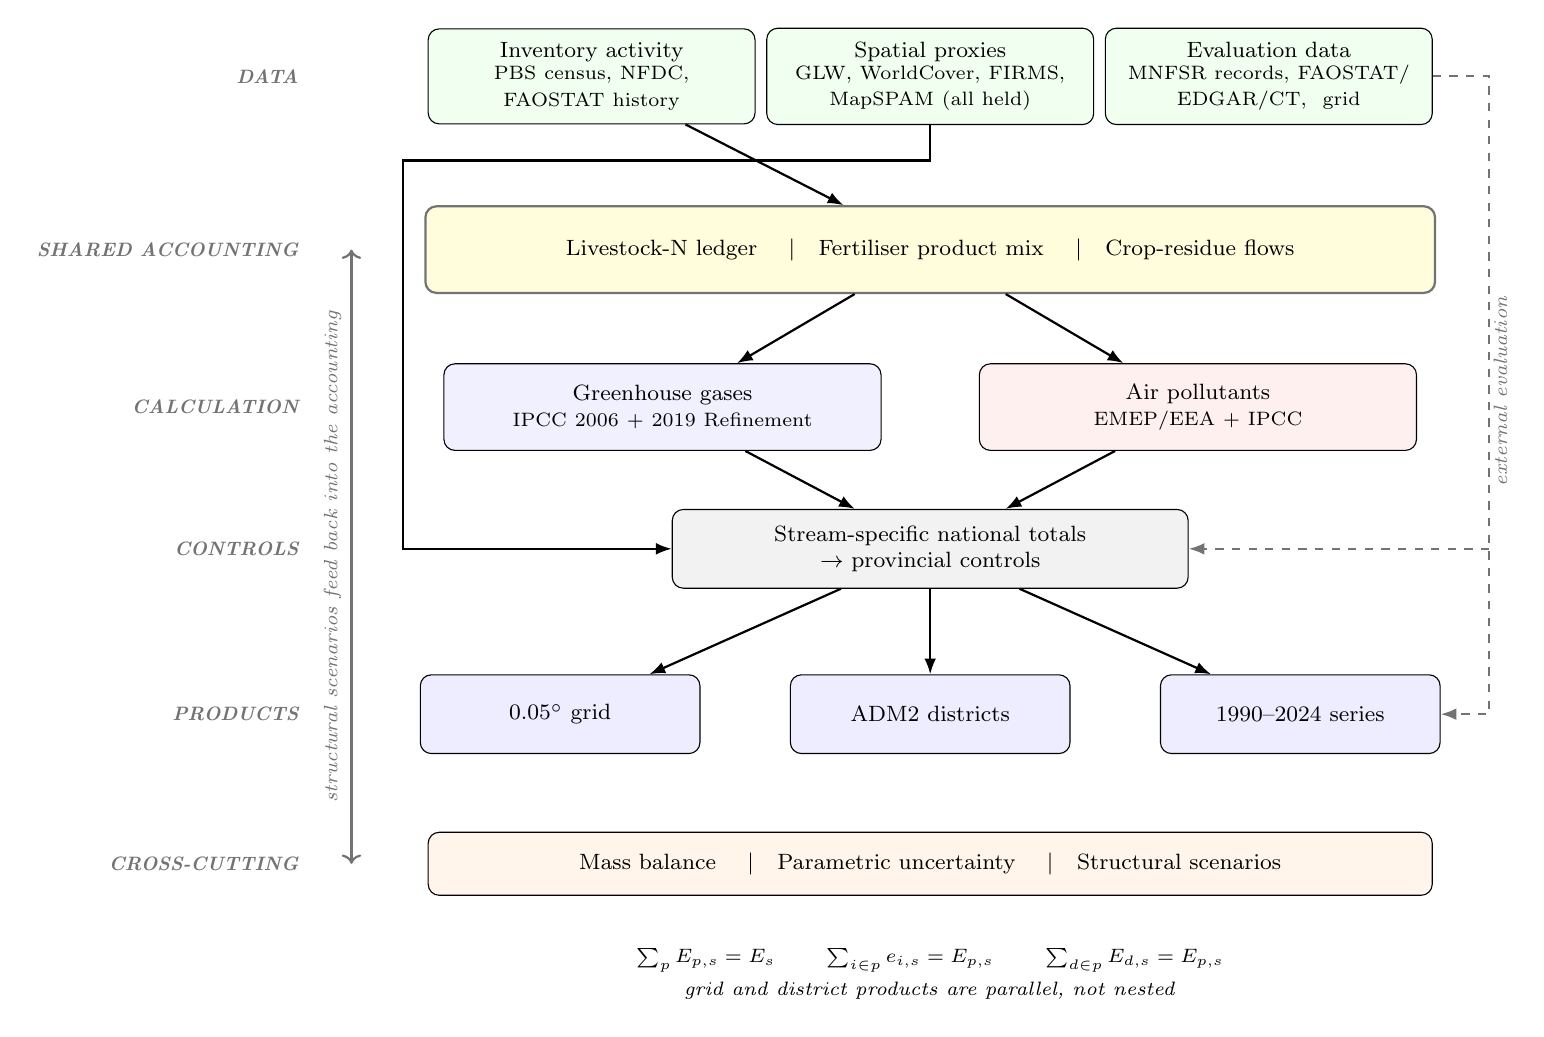
\begin{tikzpicture}[
  font=\footnotesize,
  band/.style={font=\scriptsize\bfseries\itshape, anchor=east, text=black!55},
  data/.style={draw,rounded corners,align=center,inner sep=5pt,fill=green!6,minimum height=11mm,
               text width=38mm},
  ledger/.style={draw,rounded corners,align=center,inner sep=6pt,fill=yellow!14,thick,
                 draw=black!55,text width=124mm,minimum height=11mm},
  calc/.style={draw,rounded corners,align=center,inner sep=5pt,minimum height=11mm,text width=52mm},
  ctrl/.style={draw,rounded corners,align=center,inner sep=5pt,fill=gray!10,minimum height=10mm,
               text width=62mm},
  prod/.style={draw,rounded corners,align=center,inner sep=5pt,fill=blue!7,minimum height=10mm,
              text width=32mm},
  cross/.style={draw,rounded corners,align=center,inner sep=5pt,fill=orange!8,text width=124mm,
                minimum height=8mm},
  arr/.style={-{Latex[length=2mm]},thick},
  ev/.style={-{Latex[length=2mm]},thick,dashed,black!55}
]
% ---- band 1: data, separated by function ----
\node[band] at (-3.6,7.4) {DATA};
\node[data] (act)  at (0,7.4)   {Inventory activity\\\scriptsize PBS census, NFDC,\\FAOSTAT history};
\node[data] (prox) at (4.3,7.4) {Spatial proxies\\\scriptsize GLW, WorldCover, FIRMS,\\MapSPAM (all held)};
\node[data] (eval) at (8.6,7.4) {Evaluation data\\\scriptsize MNFSR records, FAOSTAT/\\EDGAR/CT, \NHthree{} grid};

% ---- band 2: shared accounting ----
\node[band] at (-3.6,5.2) {SHARED ACCOUNTING};
\node[ledger] (led) at (4.3,5.2)
  {Livestock-N ledger \quad$|$\quad Fertiliser product mix \quad$|$\quad Crop-residue flows};

% ---- band 3: two calculations ----
\node[band] at (-3.6,3.2) {CALCULATION};
\node[calc,fill=blue!6]  (ghg) at (0.9,3.2) {Greenhouse gases\\\scriptsize IPCC 2006 + 2019 Refinement};
\node[calc,fill=red!6]   (air) at (7.7,3.2) {Air pollutants\\\scriptsize EMEP/EEA + IPCC};

% ---- band 4: controls and products ----
\node[band] at (-3.6,1.4) {CONTROLS};
\node[ctrl] (ctrl) at (4.3,1.4) {Stream-specific national totals\\$\rightarrow$ provincial controls};
\node[band] at (-3.6,-0.7) {PRODUCTS};
\node[prod] (grid) at (-0.4,-0.7) {\SI{0.05}{\degree} grid};
\node[prod] (dist) at (4.3,-0.7)  {ADM2 districts};
\node[prod] (ts)   at (9.0,-0.7)  {1990--2024 series};

% ---- cross-cutting ----
\node[band] at (-3.6,-2.6) {CROSS-CUTTING};
\node[cross] (cc) at (4.3,-2.6)
  {Mass balance \quad$|$\quad Parametric uncertainty \quad$|$\quad Structural scenarios};

\draw[arr] (act) -- (led);
\draw[arr] (led) -- (ghg);
\draw[arr] (led) -- (air);
\draw[arr] (ghg) -- (ctrl);
\draw[arr] (air) -- (ctrl);
\draw[arr] (ctrl) -- (grid);
\draw[arr] (ctrl) -- (dist);
\draw[arr] (ctrl) -- (ts);
% proxies drive the allocation, not the accounting: route down the left margin so the
% arrow does not cut through the shared-ledger or calculation boxes
\draw[arr] (prox.south) -- ++(0,-0.45) -| (-2.4,1.4) -- (ctrl.west);
\draw[arr,black!55,<->] (-3.05,-2.6) -- (-3.05,5.2)
  node[midway,rotate=90,anchor=south,font=\scriptsize\itshape,text=black!55]
  {structural scenarios feed back into the accounting};

% evaluation: short dashed arrows onto the products they evaluate
\draw[ev] (eval.east) -| (11.4,-0.7) -- (ts.east);
\draw[ev] (11.4,1.4) -- (ctrl.east);
\node[rotate=90,font=\scriptsize\itshape,text=black!55,anchor=south] at (11.75,3.4)
  {external evaluation};

\node[font=\scriptsize,align=center] at (4.3,-4.0)
  {$\sum_{p} E_{p,s} = E_{s}$ \qquad $\sum_{i\in p} e_{i,s} = E_{p,s}$
   \qquad $\sum_{d\in p} E_{d,s} = E_{p,s}$\\[1mm]
   \emph{grid and district products are parallel, not nested}};
\end{tikzpicture}%
}
\caption{%
Official activity data feed a shared livestock-nitrogen, fertiliser-nitrogen and crop-residue
accounting system. Separate greenhouse-gas (\CHfour{}, \NtwoO{}, \COtwo{}) and air-pollutant
(\NHthree{}, \NOx{}, PM$_{2.5}$, CO, NMVOC, BC, SO$_2$) calculations produce stream-specific
national totals, which become provincial controls and are allocated independently to a
\SI{0.05}{\degree} grid and to ADM2 districts on process-matched proxies; every product reconciles to
its control. Dashed arrows denote external evaluation, which is applied to the products rather than
to the calculations. Evaluation data are never used as inventory inputs.
}
\label{fig:overview}
\end{figure*}

% ===========================================================================
\section{Related Work}
\label{sec:related_work}
% ===========================================================================

\subsection{National inventory methods}

National agricultural inventories generally follow the 2006 IPCC Guidelines
\citep{ipcc2006} and, increasingly, the 2019 Refinement \citep{ipcc2019}, which updated
several agricultural emission factors and introduced climate-specific disaggregation for
soil nitrous oxide.

The IPCC framework defines several methodological tiers. Tier~1 combines default emission
factors with national activity data. Tier~2 replaces selected defaults with
country-specific parameters or more detailed activity characterisation. Tier~3 uses
higher-order models or direct national measurement systems.

Pakistan's national agricultural inventories have been prepared mainly with Tier~1 methods
and national activity totals \citep{gcisc,mir2022}. This approach supports comprehensive
national reporting but provides limited information about subnational patterns or
individual processes.

\subsection{Global gridded inventories}

Several international datasets provide independent estimates of agricultural emissions for
Pakistan. FAOSTAT calculates national agricultural and land-use emissions from FAO activity
data using mainly IPCC Tier~1 methods and reports results by category and gas
\citep{faostat,tubiello2013}.

EDGAR provides national totals and gridded emissions at approximately \SI{0.1}{\degree}
resolution using a globally consistent methodology \citep{edgar2025booklet,crippa2020};
this paper's comparison table keeps one row from the prior 2024-vintage booklet
\citep{edgar2024} because the 2025 release revised Pakistan's agricultural
\CHfour{} history and the revision itself is informative. Climate
TRACE reports country- and subsector-level agricultural emissions using a combination of
inventories, models and observation-informed methods \citep{climatetrace}.

These products provide useful external reference points, but they are not substitutes for a
nationally compiled inventory. They generally use globally harmonised or model-derived
assumptions and may not incorporate the most appropriate national activity data or system
definitions. In this study, they are used as external benchmarks rather than as reported
national values.

\subsection{Spatial allocation of emissions}

Allocating national or subnational emissions to a grid is a dasymetric-mapping problem. An
emission total is distributed according to a spatial proxy that represents the location or
intensity of the underlying activity. Similar approaches are widely used in fossil-CO$_2$
inventories and global emissions gridmaps \citep{oda2018,crippa2020}.

Several open datasets provide relevant agricultural proxies. The Gridded Livestock of the
World (\GLW{}) dataset provides modelled species-specific livestock densities
\citep{glw4,gilbert2018}. The Spatial Production Allocation Model (MapSPAM) provides
crop-specific physical areas \citep{mapspam2020}. ESA WorldCover provides a
\SI{10}{\metre} land-cover classification \citep{worldcover2021}, while NASA FIRMS and
other satellite products identify active fires and burned areas \citep{firms,giglio2016}.

The quality of a spatial inventory depends on whether each proxy represents the process
being allocated. Livestock density is appropriate for emissions produced directly by
animals, paddy area for rice methane, cropland for fertiliser-related emissions, and
satellite fire occurrence for the location of residue burning. A single proxy applied to an
entire inventory category may misallocate emissions when that category contains several
distinct activity streams.

A further requirement is mass conservation. Some spatial inventories distribute emissions
without subsequently rescaling the mapped values to the original control total. In such
cases, the gridded product may no longer reproduce the national or provincial inventory.
The framework developed here treats reconciliation as an invariant: every mapped emission
stream must sum to its corresponding control total.

\subsection{Agricultural ammonia inventories}

Agricultural ammonia inventories have largely developed within the air-quality community,
separately from greenhouse-gas inventories used for climate reporting. The EMEP/EEA
Guidebook represents livestock ammonia through a stage-resolved mass flow. Total ammoniacal
nitrogen is tracked through grazing, housing, yards, storage and field application, with
emission factors varying by animal category and manure-management system
\citep{emep2023manure}.

This process resolution is needed because ammonia losses occur at specific stages of manure
handling. By contrast, Tier~1 greenhouse-gas methods often represent manure nitrogen using
annual fractions that aggregate across several stages. Combining the two frameworks
therefore requires careful alignment of their system boundaries and nitrogen pools.

\citet{sanh2026} provide a regional reference for South Asia. Their framework estimates
agricultural \NHthree{} emissions for the SAARC countries across five sectors using an
explicit nitrogen-flow model and provides an openly available \SI{0.1}{\degree} grid
\citep{sanh2026data}. We use this inventory to compare both the national magnitude and the
spatial pattern of our ammonia estimates.

Other global products, including EDGAR and HTAP, also cover Pakistan. However, they are
built without national activity data and rely partly on the same underlying FAO statistics
used by many national and regional inventories. They therefore provide useful bounds and
methodological comparisons, but agreement with them does not constitute fully independent
confirmation.

\subsection{Crop-residue burning inventories}

Crop-residue burning can be estimated using two broad approaches. Bottom-up inventories
calculate the mass burned from crop production, residue-to-product ratios, dry-matter
fractions, combustion factors, and the proportion of residues burned. National
greenhouse-gas inventories generally use this approach, and the burned fraction is its
dominant uncertainty.

Top-down or observation-based approaches use satellite fire detections, fire radiative
power, or burned-area products. These datasets provide much stronger information about the
location and timing of fires, but conversion to burned mass depends on additional
assumptions and also carries substantial uncertainty.

This study uses the two types of information for separate purposes. The national quantity
burned is calculated using a bottom-up inventory, while satellite fire detections are used
only to allocate that quantity spatially. Satellite detections therefore determine the
mapped distribution but do not provide an independent estimate of the national total, a
distinction that matters because the two are sometimes conflated.

\subsection{Contribution relative to previous work}

Compared with conventional national inventory workbooks, this framework integrates
calculation, uncertainty analysis, spatial allocation, external evaluation and historical
reconstruction in a reproducible codebase. Compared with global gridded products, it uses
nationally grounded activity data and province-level control totals within a hybrid
Tier~1/Tier~2 agricultural inventory.

Its main contribution is the combination of these elements. The national inventory
establishes the emission totals, process-specific proxies determine their spatial
distribution, and exact reconciliation keeps the provincial, gridded and district products
consistent with the reported figures. To our knowledge, this combination has not previously
been implemented for Pakistan's agricultural sector.

% ===========================================================================
\section{Study Area and Data}
\label{sec:data}
% ===========================================================================

\subsection{Study area}

Agriculture in Pakistan is concentrated in the irrigated Indus basin, which extends through
Punjab and Sindh and supports most of the country's crop and livestock production.
Approximately four-fifths of Pakistan's cropland is irrigated through canals and tube wells.
The country also has a large livestock population, with buffalo accounting for a substantial
share, and is among the world's largest consumers of urea fertiliser.

These characteristics shape both the composition and the geography of agricultural
emissions. Enteric fermentation and soil nitrous oxide dominate the greenhouse-gas
inventory, while emissions are spatially concentrated in the irrigated canal belt.

\subsection{Activity data}

National activity data are drawn primarily from official Pakistani sources. Livestock
populations are taken from the 2024 PBS 7th Agricultural Census \citep{pbscensus2024}. The
Pakistan Economic Survey \citep{econsurvey2024ag} is used as a cross-check. The two sources are
not expected to match exactly because the census is based on enumeration, whereas the
Economic Survey includes projections derived from earlier census rounds.
Within the census itself the national summary table and the district tables are separate
transcriptions, and they differ by a handful of head in two species. Neither is edited to force
agreement: the national table is the emissions control, the district tables drive the spatial
allocation, and the residual per species is published with the normalisation factor it implies in
\texttt{outputs/agriculture\_livestock\_reconciliation\_2024.csv}.

Crop area and production data are taken from the Pakistan Economic Survey's Agriculture
chapter for FY2023--24 \citep{econsurvey2024ag} and PBS agricultural statistics.
Synthetic-nitrogen offtake is the audited full-year figure from the National Fertilizer
Development Centre's Fertilizer Review for the same year \citep{nfdc2024}. Both documents are
archived in this repository; the citations name the editions the engine reads, not the most
recent editions published. FAOSTAT activity series are used to reconstruct emissions
for 1990--2023, while the 2024 inventory is anchored to the latest Pakistani census and
administrative data \citep{faostat}.

\subsection{Geospatial data}

Spatial allocation uses the open global datasets listed in Table~\ref{tab:data}.

Livestock emissions are allocated using species-specific densities from Gridded Livestock of
the World~4 \citep{glw4}. Rice-related emissions ride MapSPAM~2020 physical rice
area \citep{mapspam2020}: the raster (V2r2) is held and hash-pinned since the
spatial facility program, its former cropland-fallback class deleted from the
allow-list so a checkout without it refuses the build, and the own-year GCD-Rice
2023 classification is published beside it as a crosscheck and a priced
district-level bracket. Crop-residue
burning is allocated using NASA FIRMS VIIRS
active-fire detections from the reporting period's own burning windows
\citep{firms}. The held record spans all nine fiscal years---\num{1664876} unique
detections fetched over per-crop burning windows derived from the FAO crop calendar's
own harvest dates (rice, wheat, cotton, maize and sugarcane, each harvest followed by a
45-day residue-clearing tail, clipped to its fiscal year)---but the spatial surface
consumes only the reporting period's own dates, \num{166393} in-grid detections inside
FY2023--24. Period-matching is a correction this series already made once (an earlier
extraction spanned October 2024--May 2025, one season after the period, and that offset
was declared until the period-matched extraction replaced it), so the nine-year record
is deliberately not pooled into a climatology here: each year's fires allocate only
that year. The window shapes only the within-province fire geography, never a
magnitude.

The fire layer's construction is stated in full so its declared choices are reviewable.
The product is the science-quality \texttt{VIIRS\_SNPP\_SP} archive, requested in
five-day spans (the area API's maximum) over the national bounding box; detections
are deduplicated on (latitude, longitude, acquisition date).
Each detection is weighted by fire radiative power plus one---FRP approximates biomass
burned, and the offset keeps zero-FRP detections from vanishing. Two filters are
deliberately \emph{not} applied to this spatial surface, and their absence is a
declared choice rather than an
omission: no confidence filter (every detection at any confidence enters the surface)
and no crop mask (the only mask is the national boundary, so non-agricultural fires
inside Pakistan contribute weight where they burn). The monthly timing layer is
stricter: there an attribution ladder masks the bounding box's Indian-Punjab
detections, excludes persistent detections within \num{0.01}\si{\degree} of the kiln
registry's coordinates, and keeps cropland detections only---of the \num{169657}
detections in FY2023--24, \num{103747} fall outside Pakistan, \num{4102} sit near
kilns, \num{9380} off cropland, and \num{52428} are attributed to residue burning; the
unattributed counts are published in the burning crosscheck, never forced into the
profile. A district shape carrying
residue-burning mass in which the layer records no fire falls back to a uniform spread
within that shape, declared per event in the grid fallback ledger; a fetch returning
zero detections refuses to write at all, so an empty fire layer can never look
fetched. Other
cropland-related streams are allocated using the cropland fraction from ESA WorldCover~2021
\citep{worldcover2021}.

Provincial boundaries are obtained from geoBoundaries \citep{runfola2020}, while district
boundaries are based on GADM or GAUL ADM2 polygons. District allocations are evaluated
against crop-area statistics published by the Ministry of National Food Security and
Research \citep{mnfsrcrops}. National emission totals are compared with FAOSTAT, EDGAR and
Climate TRACE.

\begin{table}[!htbp]
\centering
\footnotesize
\begin{tabularx}{\linewidth}{@{}llX@{}}
\toprule
\textbf{Dataset} & \textbf{Use} & \textbf{Role} \\
\midrule
PBS 7th Ag.\ Census & activity & livestock, crop area \\
Economic Survey & activity & crops, livestock cross-check \\
NFDC & activity & synthetic nitrogen \\
FAOSTAT (QCL/RFN/GT) & activity/bench. & time series, benchmark \\
EDGAR 2024/2025 & benchmark & independent national totals \\
Climate TRACE v7.1.9 & benchmark & independent national totals \\
MNFSR district crops & records & district validation (rice, wheat) \\
\GLW{} (2020) & proxy & livestock density \\
MapSPAM 2020 & proxy (held, hash-pinned) & rice area \\
ESA WorldCover 2021 & proxy & cropland fraction \\
NASA FIRMS (VIIRS) & proxy & fire occurrence \\
geoBoundaries / GADM & boundary & province / ADM2 district polygons \\
\bottomrule
\end{tabularx}
\caption{Principal datasets used in the inventory. Pakistani official statistics provide
the national and administrative activity data. Open global products provide spatial proxies
and external benchmarks. Inputs used only in the exploratory land-sector extension are
listed in Supplementary Note~S1.}
\label{tab:data}
\end{table}

\subsection{Status of the estimates}

The estimates remain provisional wherever this inventory holds no nationally measured
parameter. The
livestock population is anchored to the 2024 agricultural census, but the dairy-cattle share
is derived from FAOSTAT milk-animal counts. Rice harvested area and several agronomic
fractions are based on published literature or default assumptions pending national survey
data. Each such parameter is identified in the input files and carried through the resulting
outputs and uncertainty analysis.

% ===========================================================================
\section{Methods}
\label{sec:methods}
% ===========================================================================

The framework consists of four main stages: calculation of the national agricultural
inventory; allocation of national totals to provinces; allocation to a \SI{0.05}{\degree}
grid and to administrative districts; and uncertainty, key-category, completeness and
quality-control analysis.

The inventory is predominantly Tier~1. Each category uses the equations in the 2006 IPCC
Guidelines, together with relevant updates from the 2019 Refinement, and applies them to
country-specific activity data. Selected livestock parameters provide partial Tier~2
characterisation where nationally appropriate values are available. These include typical
animal masses, the dairy-cattle share and manure-management-system shares.

Tier status is reported by category in Table~\ref{tab:tierstatus}. This is more informative
than assigning one tier to the entire inventory, because the level of country-specific
detail differs among categories.

All activity values, emission factors and parameters are stored in version-controlled data
files; values are not embedded directly in the calculation code. Greenhouse gases are
converted to carbon-dioxide equivalents using AR5 100-year global-warming potentials ---
28 for \CHfour{} and 265 for \NtwoO{} --- to match the Common Reporting Table convention.
AR6-equivalent totals are reported separately.

\begin{table}[!htbp]
\centering
\footnotesize
\setlength{\tabcolsep}{4pt}
\begin{tabular}{@{}lp{0.26\linewidth}p{0.34\linewidth}@{}}
\toprule
\textbf{Category} & \textbf{Method / data} & \textbf{Country-specific elements} \\
\midrule
Enteric fermentation & T1 method, CS data & species census, dairy split \\
Manure management & T1/2, CS data & animal mass, Nex, MMS, temp.\ zone \\
Managed soils & T1 method, CS data & fertiliser data, dry-climate EFs \\
Rice cultivation & T1 method, CS data & area, cultivation period \\
Field burning & T1 method, CS data & crop production, residue params \\
Urea application & T1 method, CS data & urea offtake; N series before 2024 \\
\bottomrule
\end{tabular}
\caption{Method-tier status by category. All categories use the Tier-1 (T1)
method equations on country-specific (CS) activity data; manure management is
partly Tier~2 through country-specific animal mass and management-system shares.
No emission factor is Tier~3 (Pakistani field measurement).}
\label{tab:tierstatus}
\end{table}

\subsection{National inventory}

\paragraph{Enteric fermentation and manure management}
Enteric methane is calculated using the Tier~1 form of IPCC Eq.~10.19,
\begin{equation}
\mathrm{CH_4^{ent}} \;=\; \sum_t N_t\, EF_t \times 10^{-6},
\end{equation}
where $N_t$ is the population of livestock category $t$ and $EF_t$ its annual per-head
methane emission factor.

Methane from manure management is calculated using IPCC Eq.~10.22 with temperature-dependent
factors, and direct nitrous oxide from manure management follows Eq.~10.25. Nitrogen
excretion is calculated as $N_{\mathrm{rate},t} \times TAM_t \times 365/1000$, where
$N_{\mathrm{rate},t}$ is the daily nitrogen-excretion rate and $TAM_t$ is typical animal
mass.

The calculation then distributes excreted nitrogen among manure-management systems. Dung
burned as household fuel is assigned to the energy sector and excluded from the agricultural
inventory to prevent double counting. Nitrogen deposited directly on pasture is assigned to
managed soils rather than to manure management.

\paragraph{Managed soils}
Direct soil nitrous oxide follows IPCC Eq.~11.1,
\begin{equation}
\mathrm{N_2O^{direct}} \;=\;
\left[(F_{\mathrm{SN}}+F_{\mathrm{ON}}+F_{\mathrm{CR}})\,EF_1
+ F_{\mathrm{PRP}}\,EF_{3,\mathrm{PRP}}\right]\frac{44}{28},
\end{equation}
where $F_{\mathrm{SN}}$, $F_{\mathrm{ON}}$, $F_{\mathrm{CR}}$ and $F_{\mathrm{PRP}}$ are
nitrogen inputs from synthetic fertiliser, organic amendments, crop residues and pasture
deposition respectively.

Nitrogen applied to rice is assigned the flooded-rice emission factor
$EF_{1,\mathrm{FR}}$. Indirect \NtwoO{} from volatilisation and leaching follows IPCC
Eqs.~11.9 and~11.10.

For direct \NtwoO{} from non-rice cropland, the reference retains the 2019 dry-climate value $EF_1=0.005$ as a conditional factor transfer. Aridity alone does not establish its applicability to irrigated cropland. Rice and grazing use their separate source formulations, and aggregate/climate alternatives remain structural sensitivities. Agreement with an external inventory is not used to select the factor.

\paragraph{Rice cultivation, residue burning and urea application}
Rice methane is calculated using IPCC Eqs.~5.1 and~5.2,
\begin{equation}
\mathrm{CH_4^{rice}} \;=\; \sum_i EF_c\, SF_{w,i}\, SF_{p,i}\, SF_{o,i}\, t_i\, A_i
\times 10^{-6},
\end{equation}
where $EF_c$ is the baseline daily emission factor, $SF_w$ represents the water regime,
$SF_p$ the pre-season water regime, $SF_o$ the effect of organic amendments, $t_i$ the
cultivation period and $A_i$ the harvested area.

Emissions from field burning follow the generic biomass-burning equation in the IPCC
Guidelines. Urea-application \COtwo{} follows Eq.~11.13. The urea mass has two bases, and
each year states which it used in \texttt{outputs/agriculture\_urea\_basis.csv}. For the
reference year it is the national urea offtake NFDC prints for the fiscal year itself. For
every earlier year, which has a total-nitrogen figure and no published product split, it is
reconstructed from that series by a constant chemical relation. The reconstruction was
formerly applied to the reference year as well, where it fell short of the printed offtake by
\SI{0.207}{\percent}; a measurement is preferred to an approximation of it wherever one
exists, and the approximation is retained, and labelled, where none does.

Liming emissions under category 3.G are not estimated: no national lime-use activity figure
has been sought. Liming is recorded as ``not estimated'' in the completeness
assessment.

\subsection{Provincial allocation}

National emission streams are allocated to the four provinces and a small residual region
using activity-specific administrative shares.

Enteric fermentation, manure-management emissions and pasture-deposited nitrogen use
provincial livestock-census shares. Rice methane and rice-specific fertiliser nitrogen use
provincial rice area. Residue-related emissions use cropland shares. Synthetic-fertiliser
\NtwoO{} and urea \COtwo{} use provincial fertiliser-offtake shares.

Applied manure requires a different treatment, because it is generated near livestock but
applied to cropland. Its provincial distribution is therefore derived by intersecting
cropland with livestock density at the grid-cell level and then aggregating the resulting
surface to provinces.

All provincial shares are normalised to sum to one. Provincial estimates therefore reproduce
the national control total exactly.

\subsection{Gridded allocation and mass-balance reconciliation}

Each provincial emission stream is allocated to a \SI{0.05}{\degree} grid using dasymetric
weighting. Let $E_{p,s}$ be the control total for emission stream $s$ in province $p$, let
$\Omega_p$ be the set of grid cells within that province, and let $w_{i,s}$ be the
spatial-proxy value for cell $i$. Emissions in each cell are calculated as
\begin{equation}
e_{i,s} \;=\; E_{p,s}\,\frac{w_{i,s}}{\sum_{j\in\Omega_p} w_{j,s}},
\qquad i\in\Omega_p .
\label{eq:reconcile}
\end{equation}
This construction guarantees that $\sum_{i\in\Omega_p} e_{i,s}=E_{p,s}$. The grid therefore
reconciles to the provincial total, and provincial totals reconcile to the national
inventory.

Spatial proxies are assigned by emission stream rather than by broad inventory category.
This distinction matters because a single category can contain several nitrogen or activity
streams with different geographies.

\GLW{} livestock density is used for enteric methane, manure-management emissions and
pasture-deposited nitrogen. Species densities are weighted by their per-head emission
factors, so that the resulting proxy represents the spatial distribution of emissions rather
than unweighted animal numbers.

MapSPAM paddy area is the declared proxy for rice methane and the rice-specific
fertiliser stream; the raster (2020 V2r2, hash-pinned) is held and consumed since
the spatial facility program, its cropland-fallback class deleted fail-closed,
and the own-year GCD-Rice 2023 classification ships beside it as a published
crosscheck and a priced district-level bracket (Section~\ref{sec:data}). FIRMS
active-fire detections are used for crop-residue burning. WorldCover cropland fraction is
used for synthetic fertiliser, crop-residue inputs to soils and urea application.

Managed soils are constructed by allocating each nitrogen input separately and then summing
the resulting stream-level surfaces. This prevents the geography of synthetic fertiliser
from being imposed on manure-derived or pasture-derived nitrogen.

Applied manure is allocated using cropland weighted by livestock density. This proxy
represents two physical constraints: manure is applied on agricultural land, but transport
costs generally keep it close to the herd that produces it.

Where a proxy has no positive values within a province, the corresponding emission stream is
distributed uniformly across that province. This fallback preserves the provincial control
total.

\subsection{District allocation and historical district panel}
\label{sec:methods-district}

The same proportional-allocation rule is used to distribute provincial totals among
administrative districts. The main output contains 116 districts across the four provinces.
Gilgit-Baltistan, Azad Jammu and Kashmir, and Islamabad Capital Territory are represented
together as a residual unit, producing 115 reporting units in total.

For most emission streams, district shares are obtained by summing the relevant spatial
proxy within each district and normalising those sums within the province.

Livestock categories receive a more direct treatment: livestock emissions are distributed
using district head-counts from the 2024 PBS Agricultural Census, every census district
resolved through the inventory's canonical district crosswalk (several census districts
sum onto one boundary polygon where the boundary file predates a split). The two census
units the boundary file does not draw, Cholistan Area and Larkana District, keep their own
share as named rows of the district panel and fall to the province surface in the grid; a
polygon the census does not reach is a build failure, not a proxy.

The gridded and district products are parallel allocations of the same provincial controls.
They are not nested representations of one another. The \SI{0.05}{\degree} grid uses
continuous gridded proxies, whereas the district table substitutes census head-counts for
livestock where possible. Both products reconcile to the same provincial and national
totals, but summing grid cells within a district will not necessarily reproduce the
census-controlled district estimate. Formally,
$\sum_{i\in\Omega_p}e_{i,s}=E_{p,s}$ for the grid and $\sum_{d\in p}E_{d,s}=E_{p,s}$ for the
district product, and both satisfy $\sum_p E_{p,s}=E_s$.

No consistent multi-year district activity dataset is available. The historical district
panel therefore holds the audited 2024 district shares fixed and rescales them to each year's
national category total for 1990--2024.

The district values consequently follow the national time series. They do not represent
observed changes in the geographic distribution of activity over time. This assumption is
evaluated in Section~\ref{sec:limitations}.

The exploratory land-sector extension in Supplementary Note~S1 is excluded from the
agricultural totals, benchmarking, key-category assessment and uncertainty analysis.

\subsection{Uncertainty analysis}

Uncertainty is estimated using two propagation approaches applied to the same set of
activity-data and emission-factor uncertainties.

IPCC Approach~1 propagates uncertainty analytically. Uncertainties in multiplicative terms
are combined in quadrature, while uncertainties in additive components are combined using
their contributions to the total.

The Monte-Carlo analysis samples the \emph{components}: each engine row is drawn from a
mean-preserving lognormal at its own declared width---appropriate for non-negative
emissions with potentially right-skewed uncertainty---with one shared deviate per
declared correlation group, so rows split apart for allocation reasons cannot average
their common error away. The simulation uses $10^4$ iterations, and the category and
sector totals are the \emph{sums of the sampled rows} in every realisation rather than
sampled quantities in their own right.

The two approaches test the sensitivity of the reported interval to the form of propagation.
They do not provide independent estimates, because both use the same underlying uncertainty
assumptions. Agreement between them therefore indicates consistency between analytical
quadrature and lognormal aggregation.

Managed-soils components that share an emission factor are treated as perfectly correlated.
This applies to separate volatilisation and leaching streams that appear as distinct rows
because they use different spatial proxies. Treating them as independent would artificially
reduce uncertainty when one physical stream is divided into several reporting components.

Other within-category and cross-category correlations are not modelled \emph{by this
sector-scoped stream}, and the qualifier matters because a second engine treats two of them
differently. This sector's Monte Carlo samples component totals, which cannot express
covariance between the categories its stages couple; the NATIONAL run instead samples a
parameter graph, and there two physical couplings are carried explicitly---fertiliser N as
one audited series driving both the soils components and the urea term, and each species'
head-count shared between its enteric and manure components. Their effect at national scale
is about a hundredth of a percentage point, in the widening direction. Supplementary
Note~S3 gives that treatment; the limitation of the sector-scoped stream is the one stated
here. The reported
national interval therefore reflects the documented parameter uncertainties under this
correlation structure. Factor-level uncertainties are reported in
Table~\ref{tab:ef-full}, category distributions in \ref{app:unc}, and full input
provenance in Supplementary Note~S3.

\subsection{Key categories, completeness and quality control}

Key categories are identified using the IPCC Approach~1 level and trend assessments.

The level assessment ranks categories by their contribution to the absolute national total
in the reference year. The trend assessment uses
$T_x = L_{x,0}\,\lvert g_x - g_{\mathrm{tot}}\rvert$, where $L_{x,0}$ is category $x$'s
share in the base year, $g_x$ is its growth since 1990 and $g_{\mathrm{tot}}$ is the growth
of the total agricultural inventory. The metric therefore identifies categories that are
both important in the base year and whose trajectory differs from the sector average. It
should not be interpreted simply as a category growth rate.

Categories are accumulated until the \SI{95}{\percent} threshold is reached. A category is
classified as key if it qualifies under either the level or the trend assessment.

Inventory coverage is documented through a completeness table. Every \AFOLU{}
category-and-gas combination receives an IPCC notation key: estimated, not estimated, not
occurring, or included elsewhere. This makes known gaps, exclusions and cross-sector
transfers explicit.

Quality control is implemented through automated tests covering units, source traceability,
mass-balance reconciliation, benchmark ranges, and consistency among national, provincial,
grid, district and historical outputs. Quality assurance is supported through comparison
with FAOSTAT, EDGAR, Climate TRACE and independent district statistics. Changes to activity
data, emission factors or methods trigger recalculation of the complete time series.

% ===========================================================================
\section{Emission Factors and Calculated Emissions}
\label{sec:ef}
% ===========================================================================

The spatial allocation described in Section~\ref{sec:methods} determines where emissions are
placed but does not change their national magnitude. National totals are determined only by
the activity data and the emission factors.

Table~\ref{tab:ef-full} reports the principal emission factors, their uncertainty, and their
IPCC or literature source. Table~\ref{tab:tier2} reports the country-specific and
inventory-specific parameters that replace or refine selected Tier~1 defaults. Full source
details and derivations are provided in Supplementary Note~S2.

Each factor is stored in a version-controlled data file together with its units, source and
uncertainty. This structure allows every calculated value to be traced to a documented
input.

\subsection{Emission factors}

Enteric-fermentation and manure-management factors are drawn mainly from the 2006 IPCC
defaults for the Indian Subcontinent. Managed-soils factors use the climate-specific values
in the 2019 Refinement.

The direct soil \NtwoO{} factor is the most consequential individual methodological choice.
The main inventory uses the dry-climate value $\EFone{}=0.005$. The older 2006 aggregate
value of $0.010$ and the 2019 wet-climate value of $0.016$ are retained as sensitivity
cases.

The dry-climate value is also close to the crop-weighted empirical estimate of approximately
$0.0055$ reported by \citet{cui2021} for Pakistan. That empirical value is used as a
sensitivity anchor, not as the operative emission factor.

Rice methane uses the IPCC baseline factor together with water-regime scaling. The main case
assumes continuously flooded conditions, $SF_w=1$. Intermittent irrigation and rainfed
conditions are evaluated as alternatives.

\begin{table}[!htbp]
\centering
\footnotesize
\begin{tabular}{@{}llrl@{}}
\toprule
\textbf{Factor (unit)} & \textbf{Value} & \textbf{$\pm$\%} & \textbf{Source} \\
\midrule
\multicolumn{4}{@{}l}{\emph{Enteric \CHfour{} (kg/head/yr; 2006 T10.10--10.11)}} \\
\quad Buffalo            & 55  & 40 & 2006 T10.10 \\
\quad Dairy cattle       & 58  & 50 & 2006 T10.11 \\
\quad Other cattle       & 27  & 50 & 2006 T10.11 \\
\quad Camels             & 46  & 50 & 2006 T10.10 \\
\quad Sheep, goats       & 5   & 50 & 2006 T10.10 \\
\addlinespace
\multicolumn{4}{@{}l}{\emph{Manure management (2006 T10.14--10.21)}} \\
\quad \CHfour{} buffalo, warm (kg/hd/yr) & 5 & 30 & 2006 T10.14 \\
\quad \CHfour{} dairy cattle, warm & 6 & 30 & 2006 T10.14 \\
\quad \NtwoO{} $EF_3$ solid/liquid (kg N/kg N) & 0.005 & 100 & 2006 T10.21 \\
\quad \NtwoO{} $EF_3$ drylot & 0.02 & 100 & 2006 T10.21 \\
\addlinespace
\multicolumn{4}{@{}l}{\emph{Rice \CHfour{} (2006 T5.11--5.13)}} \\
\quad Baseline $EF_c$ (kg/ha/day) & 1.30 & 53 & 2006 T5.11 \\
\quad $SF_w$ continuous (default) & 1.00 & 26 & 2006 T5.12 \\
\quad $SF_w$ intermittent (AWD) & 0.52 & 30 & 2006 T5.12 \\
\quad $SF_w$ rainfed     & 0.28 & 40 & 2006 T5.12 \\
\addlinespace
\multicolumn{4}{@{}l}{\emph{Managed soils (kg N\textsubscript{2}O-N/kg N; 2019 Refinement)}} \\
\quad \EFone{} dry (default) & 0.005 & 110 & 2019 T11.1 \\
\quad \EFone{} flooded rice  & 0.004 & 120 & 2019 T11.1 \\
\quad \EFone{} aggregate (sens.) & 0.010 & 90 & 2006 default \\
\quad \EFone{} empirical anchor & 0.0055 & 100 & \citet{cui2021} \\
\quad $EF_4$ volatilisation (dry) & 0.005 & 100 & 2019 T11.3 \\
\quad $EF_5$ leaching     & 0.011 & 100 & 2019 T11.3 \\
\addlinespace
\multicolumn{4}{@{}l}{\emph{Carbon amendments, burning}} \\
\quad Urea carbon (t\,C/t urea) & 0.20 & 10 & 2006 Eq.11.13 \\
\quad Residue burning \CHfour{} (g/kg d.m.) & 2.7 & 40 & 2006 T2.5 \\
\bottomrule
\end{tabular}
\caption{Principal emission and carbon factors, with factor-level uncertainty
($\pm$\%, 95\% relative half-width) and provenance. These factor uncertainties are
combined with activity-data uncertainty into the per-category values propagated in
the uncertainty analysis (Section~\ref{sec:methods}, \ref{app:unc}).
Values marked \emph{(sens.)} are used only in the sensitivity analysis
(Table~\ref{tab:sensitivity}); the empirical anchor adjudicates the soil-nitrogen
choice and is not the operative factor.}
\label{tab:ef-full}
\end{table}

\subsection{Country-specific and inventory-specific parameters}

The largest departures from global Tier~1 defaults occur in the livestock characterisation.

Population-average typical animal masses are used for dairy cattle, other cattle, buffalo
and camels---declared judgements resting on working pointers rather than cited
measurements, as Supplement~S2's provenance classes record (10 cited, 3 derived, 25
working pointers and 21 declared judgements across the 59 parameter rows). These values are generally higher than the corresponding IPCC defaults and affect
both nitrogen excretion and the division of enteric emissions among livestock groups. The
dairy-cattle share is derived from FAOSTAT counts of animals reported as being in milk.

Other national parameters determine how fertiliser and soil nitrogen are represented. These
include the proportion of synthetic nitrogen supplied as urea, the share applied to rice,
and the irrigated fraction used in the leaching calculation.

Table~\ref{tab:tier2} distinguishes among four types of parameter: national activity data,
Tier~2 characterisation, regional IPCC defaults, and inventory assumptions. This
category-by-category classification defines the methodological basis more accurately than
assigning one tier to the whole inventory.

\begin{table*}[!htbp]
\centering
\footnotesize
\begin{tabular}{@{}llll@{}}
\toprule
\textbf{Parameter} & \textbf{Value (unit)} & \textbf{Status} & \textbf{Source} \\
\midrule
Dairy (in-milk) cattle share & 0.295 & national activity datum & FAOSTAT QCL 2024 (16.98/57.54 M) \\
Typical mass, dairy cattle & 400 kg & Tier-2 characterisation & Sahiwal/crossbred; LRRD 2006 \\
Typical mass, other cattle & 225 kg & Tier-2 characterisation & Pak.\ adult zebu population avg. \\
Typical mass, buffalo & 380 kg & Tier-2 characterisation & Nili-Ravi herd avg.\ (LRRD) \\
Typical mass, camels  & 480 kg & Tier-2 characterisation & dromedary herd avg.; Khan 2025 \\
Nex, buffalo & 0.32 kg N/1000\,kg/d & regional IPCC default & IPCC 2006 T10.19 Asia \\
Nex, dairy cattle & 0.47 kg N/1000\,kg/d & regional IPCC default & IPCC 2006 T10.19 Asia \\
Warm-zone share (manure) & 0.70 & inventory assumption & Indus-plain climate zone \\
Irrigated cropland fraction & 0.80 & national activity datum & FAO AQUASTAT (19/22 Mha) \\
Rice share of synthetic N & 0.16 & national activity datum & rice 3.5/22 Mha cropped \\
Urea share of applied N & 0.80 & national activity datum & NFDC offtake \\
Rice cultivation period & 125 days & Tier-2 characterisation & PARC calendar (area-weighted) \\
\bottomrule
\end{tabular}
\caption{Country-specific and inventory-specific parameters that override IPCC
defaults. \emph{Status} distinguishes national activity data, genuine Tier-2
characterisation, regional IPCC defaults, and inventory assumptions --- so the
paper does not over-claim a uniform Tier-2 basis. Full provenance (source,
table/page, derivation, and uncertainty) for these and all other
parameters and factors --- management-system shares, dung-cake fraction, residue
ratios, water/amendment factors, volatilisation and leaching fractions, and the
soil \NtwoO{} factor set --- is given in Supplementary Note~S2.}
\label{tab:tier2}
\end{table*}

\subsection{Calculated emissions}

Applying the factors in Table~\ref{tab:ef-full} and the parameters in
Table~\ref{tab:tier2} to the national activity data produces the 2024 estimates reported in
Section~\ref{sec:results}.

The same emission-factor set is held constant throughout the 1990--2024 reconstruction.
Changes in the historical series therefore reflect changes in activity, including livestock
growth and increasing fertiliser use, rather than changes in the selected factors.

\ref{app:crt} presents the activity data, implied factors and emissions by gas for
the 1990 base year and the 2024 reporting year in a Common Reporting Table structure.

\subsection{Sensitivity to major methodological choices}
\label{sec:sensitivity}

Three assumptions account for most of the methodological sensitivity: the direct soil factor
$\EFone{}$, the rice water-regime factor $SF_w$, and the distribution of livestock manure
among management systems.

Increasing $\EFone{}$ from the main-case value of $0.005$ to the 2006 aggregate value of
$0.010$ raises the national total by \SI{11.9}{}~Mt~\COe{}. Using the empirical value of
$0.0055$ produces little change and gives a managed-soils estimate of \SI{29.7}{}~Mt, close
to that of \citet{cui2021}.

Changing the rice water regime from continuously flooded to intermittent irrigation reduces
the national total by \SI{7.9}{}~Mt~\COe{}. A fully rainfed assumption reduces it by
\SI{11.9}{}~Mt~\COe{}.

Using the GLEAM~3.0 South-Asia manure-management distribution \citep{gleam2022} raises the
national total by \SI{9.9}{}~Mt~\COe{}. Unlike the soil and rice cases, this scenario
requires a complete model run because manure management is coupled to the quantity of manure
nitrogen later applied to soils. It therefore changes both manure-management and
managed-soils emissions.

All tested scenarios remain within the main Monte-Carlo interval and do not change the
ranking of the leading emission categories.

\begin{table}[!htbp]
\centering
\footnotesize
\begin{tabular}{@{}lccc@{}}
\toprule
\textbf{Scenario} & \textbf{Rice} & \textbf{Soils} & \textbf{Total} \\
\midrule
Main case ($\EFone{}=0.005$; rice flooded) & 16.5 & 28.5 & 223.5 \\
\quad $\EFone{}=0.010$ (2006 aggregate) & 16.5 & 40.4 & 235.4 \\
\quad $\EFone{}=0.016$ (2019 wet)       & 16.5 & 54.7 & 249.7 \\
\quad $\EFone{}=0.0055$ (Cui 2021)      & 16.5 & 29.7 & 224.6 \\
\quad $EF_3PRP$ wet (2019)$^{b}$        & 16.5 & 30.3 & 225.3 \\
\quad $EF_3PRP$ aggregate (2006)        & 16.5 & 42.8 & 237.7 \\
\quad Both 2006 direct factors          & 16.5 & 54.7 & 249.6 \\
\quad Rice intermittent $SF_w=0.52$ (AWD) &  8.6 & 28.5 & 215.5 \\
\quad Rice rainfed $SF_w=0.28$          &  4.6 & 28.5 & 211.5 \\
\quad Manure GLEAM 3.0 split$^{a}$      & 16.5 & 27.6 & 233.4 \\
\bottomrule
\end{tabular}
\caption{Sensitivity of the 2024 national agricultural total (Mt~\COe, AR5) to the
principal methodological choices. $^{a}$Soil and rice alternatives can be recalculated directly because each touches a
single category and the affected terms scale linearly. The GLEAM manure-management case
requires a complete model run: the nitrogen ledger is coupled, so a different split changes how much manure nitrogen
reaches the field and moves managed soils (\SI{28.5}{} to \SI{27.6}{}~Mt) as well as manure
management (\SI{21.2}{} to \SI{32.1}{}~Mt). It is the same scenario as
Table~\ref{tab:apstruct} and reports the same total. $^{b}$The pasture factor had no
scenario beside it before this release, which was an asymmetry rather than a judgement: it is
the larger lever of the two soils factors---the 2019 Refinement cut the cattle value tenfold
from the 2006 default where it halved \EFone{}---and it carries two-thirds of the difference
against FAOSTAT's managed soils. The two factor scenarios are disjoint, so the combined 2006
case is their sum rather than a separate run. Raised via the GLEAM 3.0 South-Asia management-system split (a hidden
uncertainty surfaced by the cross-check, not adopted). Generated by
\texttt{src/pkinv/eval/sensitivity\_table.py}.}
\label{tab:sensitivity}
\end{table}

% ===========================================================================
\section{Shared Nitrogen Accounting and Air-Pollutant Methods}
\label{sec:methods-shared}
% ===========================================================================

The greenhouse-gas and air-pollutant calculations use a common nitrogen ledger. This ledger
tracks how excreted and applied nitrogen moves through manure management, grazing,
fertiliser application, volatilisation and soil processes.

The two inventories therefore represent different emissions from the same underlying
nitrogen flows. Aligning their system boundaries is necessary to prevent the same nitrogen
from being removed twice, retained twice, or assigned inconsistently between \NHthree{} and
\NtwoO{}.

\subsection{Alignment of the nitrogen boundaries}
\label{sec:methods-ledger}

The reference TAN formulation follows species- and system-specific ammonia loss through housing or yard exposure, storage and field application. Each stage acts on surviving total ammoniacal nitrogen. Management NH$_3$ and NO$_x$, leaching, N$_2$ and N$_2$O losses are removed once before the surviving organic pool reaches soil. Grazing and field volatilisation remain separate pathways. The same realised pools drive indirect N$_2$O and the air species.

A separately identified IPCC alternative uses the applicable management and field volatilisation fractions. It regenerates both product families rather than combining an IPCC N$_2$O account with a different EMEP ammonia chain. Its management fractions are not additional removal from the TAN reference. Material-flow closure is tested in each configuration and uncertainty draw.

\subsection{Synthetic-fertiliser ammonia}
\label{sec:methods-air}

Synthetic-fertiliser \NHthree{} is calculated from Pakistan's reported fertiliser-product
mix rather than from one generic fertiliser composition.

EMEP/EEA factors vary substantially among products because urea and ammonium-based
fertilisers have greater volatilisation potential than nitrate-dominant products,
particularly on high-pH soils. Pakistan's alkaline cropland and urea-heavy fertiliser mix
make product weighting important.

Let $w_j$ be product $j$'s share of applied nitrogen and $EF^{\NHthree{}\text{-}N}_j$ its
ammonia-nitrogen emission factor \citep{emep2023soils}. Taking the NFDC offtake by product
\citep{nfdc2024} over one fiscal year, the product-weighted factor is
\begin{equation}
f_{\NHthree{},SF} \;=\; \sum_j w_j\, EF^{\NHthree{}\text{-}N}_j \;=\; 0.1608 .
\end{equation}
Urea supplies approximately \SI{81}{\percent} of the nitrogen in the product mix and
therefore dominates the weighted result (Table~\ref{tab:fertmix}). The remaining products
change the factor by less than 0.01.

The value 0.1608 is already expressed as kilograms of \NHthree{}-N per kilogram of nitrogen
applied. It is converted to \NHthree{} mass by the ratio $17/14$ and used directly in the
ammonia calculation. It is not multiplied by an additional \NHthree{} share.

Soil \NOx{} is calculated separately, using $f_{NO,SF}=0.007$ kg NO-N per kilogram of
nitrogen applied. For the IPCC indirect-\NtwoO{} pathway, which Eq.~11.9 defines on the
combined volatilised pool, the two are summed:
\begin{equation}
\mathrm{Frac_{GASF}} \;=\; f_{\NHthree{},SF} + f_{NO,SF} \;=\; 0.1678 ,
\end{equation}
against the IPCC ``urea-dominant'' default of 0.15. Keeping these three quantities separate
preserves the nitrogen balance and avoids applying an additional ammonia fraction to a
factor already expressed as \NHthree{}-N. Because $f_{\NHthree{},SF}$ also drives the
greenhouse-gas layer's synthetic indirect \NtwoO{}, it is resolved in one place and both
layers necessarily use it.

\begin{table*}[!htbp]
\centering
\footnotesize
\begin{tabular}{@{}lrrrrr@{}}
\toprule
\textbf{Product} & \textbf{t N} & \textbf{N content} & \textbf{Share of N}
& \textbf{$EF^{\NHthree{}\text{-}N}$} & \textbf{Contribution} \\
\midrule
Urea             & 3\,026\,265 & 0.46 & 0.8078 & 0.170 & 0.1373 \\
DAP              &   290\,777 & 0.18 & 0.0776 & 0.154 & 0.0120 \\
CAN              &   206\,058 & 0.26 & 0.0550 & 0.043 & 0.0024 \\
Other NP         &   202\,590 & 0.20 & 0.0541 & 0.154 & 0.0083 \\
Ammonium sulphate &   14\,595 & 0.21 & 0.0039 & 0.154 & 0.0006 \\
NPK              &     6\,162 & 0.15 & 0.0016 & 0.154 & 0.0003 \\
\midrule
\textbf{Total}   & \textbf{3\,746\,448} & & \textbf{1.0000} & & \textbf{0.1608} \\
\bottomrule
\end{tabular}
\caption{Derivation of the product-weighted synthetic-fertiliser ammonia factor. The table is
generated from \texttt{outputs/agriculture\_fertiliser\_composition\_2024.csv}, whose window is
exactly the twelve months July~2023 to June~2024; the annexe supplies the normalised composition
only, and the nitrogen magnitude remains the audited national offtake. NFDC's national and
provincial tables do not sum to each other over the same twelve months: the difference is
\SI{15918}{\tonne} of product, \SI{0.154917}{\percent} of the national total and mostly
urea. It is published by month and product in
\texttt{outputs/agriculture\_nfdc\_province\_residual.csv} and assigned to
Other/unallocated rather than distributed across the provinces, which would make every
residual zero and the shares look exact. Product tonnages are
NFDC offtake over one fiscal year \citep{nfdc2024}; nitrogen contents and emission factors are
EMEP/EEA values for high-pH soils, appropriate to Pakistan's alkaline cropland
\citep{emep2023soils}. \emph{All emission factors in this table are kg \NHthree{}-N per kg N
applied.} Urea carries \SI{81}{\percent} of the nitrogen and therefore dominates the weighting; the
audited national nitrogen total (\SI{3.775}{}~Mt~N) rather than this window's sum is used as the
activity datum, with the mix supplying only the composition.}
\label{tab:fertmix}
\end{table*}

\subsection{Livestock ammonia}

Livestock \NHthree{} is calculated using the EMEP/EEA total-ammoniacal-nitrogen (TAN)
mass-flow method \citep{emep2023manure,sommer2019}. The IPCC post-application fraction
$\mathrm{Frac_{GASM}}$ is not used as a livestock ammonia emission factor, because it was
developed for indirect-\NtwoO{} accounting rather than stage-resolved \NHthree{} estimation.

Excreta deposited during grazing lose a species-specific proportion of TAN directly. Manure
entering a managed system can lose ammonia during housing or yard exposure, storage and
field application. Each stage acts on the TAN remaining after the preceding stage.

The calculation distinguishes among manure systems. Solid storage passes through housing,
storage and field-application stages. Daily-spread manure reaches the field without a
storage stage. Dry lots are represented as uncovered yards.

Factors also differ among livestock categories, and are taken from Table~3-9 of the
Guidebook. Buffalo manure is assigned a TAN fraction of \num{0.50}, compared with
\num{0.60} for cattle, and a storage factor of \num{0.17} against \num{0.32}. Grazing
factors are applied to TAN rather than to total excreted nitrogen (\num{0.14} for cattle and
buffalo, \num{0.09} for small ruminants).

EMEP/EEA does not provide a separate camel category. Camels therefore use the
small-ruminant factors as the closest available published analogue, with a wider uncertainty
assigned to reflect the approximation.

\subsection{Other agricultural air pollutants}

Soil \NOx{} is estimated as approximately \SI{0.7}{\percent} of applied synthetic, organic
and crop-residue nitrogen, following \citet{stehfest2006}. The value is initially calculated
as NO-N and converted to reported \NOx{} mass using the conventional NO$_2$-equivalent
conversion.

Pollutants from crop-residue burning are calculated from the same dry-matter-burned estimate
used in the greenhouse-gas inventory. The burned mass is multiplied by the combustion factor
and by pollutant-specific emission factors for CO, PM$_{2.5}$, NMVOC, \NOx{}, \NHthree{},
black carbon and SO$_2$ (Table~\ref{tab:apef}). The PM$_{2.5}$ factor is also used by the
related satellite-nowcasting layer so that the two products report a consistent crop-burning
PM$_{2.5}$ quantity.

All air factors retain native units and source applicability. Local product-rule widths are diagnostics; the integrated conditional ensemble replays shared herd, crop, nutrient and bounded fate-factor realisations across NH$_3$, NO$_x$ and N$_2$O. Structural management shares and factor alternatives are separate cases, not confidence limits.

\begin{table}[!htbp]
\centering
\footnotesize
\setlength{\tabcolsep}{3pt}
\begin{tabular}{@{}p{0.26\linewidth}p{0.40\linewidth}rr@{}}
\toprule
\textbf{Pollutant / stage} & \textbf{Basis} & \textbf{Factor} & \textbf{$\pm$\%} \\
\midrule
\NHthree{}, synthetic fert.\ & $f_{\NHthree{},SF}$, kg \NHthree{}-N per kg N & 0.1608$^{b}$ & 30 \\
\NHthree{}, grazing & of TAN; cattle/buffalo \textbar{} small rum. & 0.14 \textbar{} 0.09 & 50 \\
\NHthree{}, housing & of TAN; cattle \textbar{} buffalo \textbar{} small rum. & 0.08 \textbar{} 0.20 \textbar{} 0.22 & 40 \\
\NHthree{}, yard (dry lot) & of TAN; dairy \textbar{} other cattle & 0.30 \textbar{} 0.53 & 50 \\
\NHthree{}, storage & of TAN surviving; cattle \textbar{} buffalo & 0.32 \textbar{} 0.17 & 40 \\
\NHthree{}, field application & of TAN surviving; cattle \textbar{} buffalo & 0.68 \textbar{} 0.55 & 40 \\
TAN fraction & of N excreted; cattle \textbar{} buffalo \textbar{} poultry & 0.60 \textbar{} 0.50 \textbar{} 0.70 & 20 \\
Soil \NOx{} & $f_{NO,SF}$, kg NO-N per kg N applied$^{a}$ & 0.007 & 100 \\
\multicolumn{4}{@{}l}{\emph{Crop-residue burning (g/kg dry matter; on $M_{burnt}\!\cdot\!C_f$)}} \\
\quad CO       & IPCC 2006 T2.5      & 92 & 40 \\
\quad PM$_{2.5}$ & \citet{akagi2011}  & 7.6 & 50 \\
\quad NMVOC    & \citet{akagi2011} / EMEP & 7.0 & 60 \\
\quad \NOx{}   & IPCC 2006 T2.5      & 2.5 & 50 \\
\quad \NHthree{} & \citet{akagi2011} & 1.3 & 60 \\
\quad BC       & \citet{akagi2011}   & 0.5 & 60 \\
\quad SO$_2$   & \citet{emep2019}    & 0.40 & 70 \\
\bottomrule
\end{tabular}
\caption{Air-pollutant factors, calculation basis, and 95\% relative uncertainty. Livestock
\NHthree{} follows the species-resolved EMEP/EEA TAN mass-flow method. Crop-burning factors are
applied to the same dry matter used in the greenhouse-gas calculation. The synthetic-fertiliser
\NHthree{} factor is already expressed as \NHthree{}-N and receives no additional
ammonia-share adjustment. Soil \NOx{} is calculated as NO-N and reported as
NO$_2$-equivalent mass.}
\label{tab:apef}
\end{table}

% ===========================================================================
\section{Evaluation Framework}
\label{sec:validation}
% ===========================================================================

The inventory is evaluated through several complementary comparisons. Each addresses a
different component of the framework.

First, national and category-level totals are compared with FAOSTAT, EDGAR and Climate TRACE
using matched years, gas metrics and category scope. These datasets provide external
reference estimates but are not direct observations of national emissions. A ratio between
0.5 and 2.0 is used as a diagnostic screening range. Values outside this range are examined
to identify differences in factors, activity data or category definitions. The range is an
operational review threshold rather than a formal statistical acceptance criterion.

Second, the model is run for 1990--2023 using FAOSTAT activity series and compared with
FAOSTAT emissions. Because the two calculations share much of their activity basis, this
comparison primarily tests the implementation and the consequences of different emission
factors. It is not an independent test of the underlying activity data.

Third, district spatial patterns are compared with independent government crop statistics
that are not used to produce the relevant district allocation. This comparison evaluates the
ranking of districts rather than their absolute emissions.

Fourth, reconciliation is tested automatically at every spatial scale. Each grid and district
product must reproduce its provincial and national control totals within numerical
tolerance. This verifies mass conservation but does not establish the accuracy of the
within-province spatial pattern.

Finally, the analytical and Monte-Carlo uncertainty calculations are compared as alternative
propagation methods. Since they use the same input assumptions, agreement between them
indicates computational consistency rather than independent confirmation.

\subsection{District comparison with independent crop records}
\label{sec:validation-district}

District allocations are evaluated against district crop-area records published by the
Ministry of National Food Security and Research \citep{mnfsrcrops}.

Spearman rank correlation is used because the comparison concerns the ordering of districts
rather than a claim that crop area directly measures emissions.

The rice-emission ranking is compared with official district rice area. Across 66 matched
districts the correlation is $\rho=0.92$ ($p<0.001$), and 13 of the 15 highest-ranked rice
districts in the inventory are among the 15 highest-ranked districts in the official data.

Managed-soils emissions are compared with district wheat area across 85 matched districts.
Wheat is used as a broad indicator of cultivated and fertilised land because it is grown
across most cropping districts. The resulting rank correlation is $\rho=0.84$.

Agreement varies geographically. It is strongest in Punjab and Balochistan and weak in
Sindh, where managed-soils emissions follow a rice-and-cotton geography that is not well
represented by wheat area alone. The Sindh result therefore reflects a limitation of the
comparison variable as well as possible uncertainty in the allocation.

Equivalent independent district checks are not possible for all categories. Livestock
emissions already use PBS district census counts where available, so comparison with the
same counts would not be independent. No comparable published district dataset was
identified for field burning or urea application. These categories are consequently recorded
as lacking independent district evaluation rather than being assigned a validation score.

\begin{table}[!htbp]
\centering
\footnotesize
\begin{tabular}{@{}lllc@{}}
\toprule
\textbf{Category} & \textbf{Independent record} & \textbf{$n$} & \textbf{Spearman $\rho$} \\
\midrule
Rice cultivation & District rice area (MNFSR) & 66 & 0.92 \\
Managed soils    & District wheat area (MNFSR) & 85 & 0.84 \\
Enteric / manure & --- (census is the proxy) & --- & n/a \\
Field burning    & --- (no district record) & --- & n/a \\
Urea application & --- (no district record) & --- & n/a \\
\bottomrule
\end{tabular}
\caption{Rank comparison between modelled district emissions and independent government
crop-area records. Rice emissions are compared with district rice area, and managed-soils
emissions with district wheat area. Categories for which the only available district
statistic is already used as an input, or for which no suitable district record exists, are
reported as not independently evaluated. Generated by
\texttt{src/pkinv/eval/validation/district\_rice\_records.py} and
\texttt{district\_records\_multi.py}; the same comparison is scored as a registered
benchmark task in \texttt{outputs/benchmark\_spatial\_allocation.csv}.}
\label{tab:distval}
\end{table}

\subsection{What each comparison shares with the engine}

External is not the same as independent, and a comparison that tuned a product cannot also
test it. Table~\ref{tab:agri-independence} states, for every comparison this section and the
release's validation catalogue carry for agriculture, what the comparison shares with the
inventory and whether it is a calibration. Three rows carry a weaker claim than they did
before this release, and in each case the reason is that the comparison reads something the
product is built from.

\begin{table*}[!htbp]
\centering
\footnotesize
\begin{tabular}{@{}p{0.22\textwidth}p{0.20\textwidth}p{0.28\textwidth}p{0.11\textwidth}p{0.08\textwidth}@{}}
\toprule
\textbf{Comparison} & \textbf{What it tests} & \textbf{Shared with the engine} &
\textbf{Independence} & \textbf{Calibration} \\
\midrule
FAOSTAT / EDGAR / CRT categories & Method and emission factors & The national activity
statistics both sides read & Partial & No \\
Cui 2021 direct-N\textsubscript{2}O & Direction of the EF1 choice & None stated; the
Pakistani value is extrapolated with no in-country observation & Partial & No \\
District rice area (MNFSR) & Spatial rank of rice emissions & Nothing: the allocation does
not read crop area & Large & No \\
District wheat area (MNFSR) & Spatial rank of managed soils & Nothing & Large & No \\
Livestock district census & --- & The census counts ARE the activity & None & No \\
NFDC monthly urea offtake & Spread between two monthly shapes & The offtake series IS the
adopted profile & None & Yes \\
VIIRS/MODIS fire detections & Attribution of detections to Pakistani cropland & The
detections ARE the burning profile's weights & None & Yes \\
FAO rice crop calendar & Plausibility of the rice window & Calendar conventions & Partial &
No \\
\bottomrule
\end{tabular}
\caption{Independence and shared-input matrix for the agriculture comparisons, in the form
the aviation paper uses. A comparison whose ``shared'' column names the product's own input
can bound allocation or attribution, and cannot confirm the quantity: the monthly fertiliser
and fire rows are calibrations for that reason, and the enteric and manure categories are
recorded above as lacking an independent district record rather than being scored against
the census that supplies them.}
\label{tab:agri-independence}
\end{table*}

% ===========================================================================
\section{Results}
\label{sec:results}
% ===========================================================================

\subsection{National greenhouse-gas inventory}

Pakistan's agricultural emissions in 2024 are estimated at \SI{223.5}{}~Mt~\COe{} using AR5
GWP-100 values. The corresponding AR6 total is \SI{218.1}{}~Mt~\COe{}.

Enteric fermentation is the largest category, contributing \SI{151.7}{}~Mt~\COe{}, or
\SI{68}{\percent} of the national agricultural total. Managed soils contribute
\SI{28.5}{}~Mt~\COe{}, followed by manure management at \SI{21.2}{}~Mt~\COe{} and rice
cultivation at \SI{16.5}{}~Mt~\COe{}. Urea application contributes \SI{4.8}{}~Mt~\COe{},
while field burning of crop residues contributes \SI{0.7}{}~Mt~\COe{}.

The inventory is therefore dominated by livestock. Enteric fermentation and manure management
together account for approximately \SI{78}{\percent} of the total. Soil and rice emissions
make up most of the remainder.

\begin{table}[!htbp]
\centering
\footnotesize
\begin{tabular}{@{}lccc@{}}
\toprule
\textbf{Category (IPCC code)} & \textbf{AR5} & \textbf{AR6} & \textbf{$\pm$\%} \\
\midrule
Enteric fermentation (3.A)   & 151.7 & 146.2 & 25 \\
Manure management (3.B)      &  21.2 &  21.0 & 33 \\
Managed soils (3.D)          &  28.5 &  29.4 & 47 \\
Rice cultivation (3.C)       &  16.5 &  16.0 & 61 \\
Urea application (3.H)       &   4.8 &   4.8 & 11 \\
Field burning (3.F)          &   0.7 &   0.7 & 45 \\
\midrule
\textbf{Agriculture total}   & \textbf{223.5} & \textbf{218.1} & \textbf{19} \\
\bottomrule
\end{tabular}
\caption{Agricultural greenhouse-gas emissions by IPCC category, 2024, reported in
Mt~\COe{} using AR5 and AR6 GWP-100 values. The uncertainty column reports the IPCC
Approach~1 \SI{95}{\percent} relative half-width.}
\label{tab:national}
\end{table}

\subsection{Comparison with international inventories}

The category-level comparison with FAOSTAT uses 2023, the latest common year, and includes
only the five agricultural categories reported by both inventories. Urea and liming are
excluded from this comparison because FAOSTAT does not report corresponding lines for
Pakistan.

The engine values compared are the calendar-2023 reconstruction of the fiscal series
(Table~\ref{tab:benchmark}), not the FY2023--24 totals reported above, which sit on a
different twelve months. For these five categories, our estimate is
\SI{207.8}{}~Mt~\COe{}, compared with \SI{233.3}{}~Mt~\COe{} in FAOSTAT. The resulting
ratio is \num{0.89}.

Agreement differs among categories. Enteric fermentation agrees to within five per cent, with a
ratio of \num{0.99}. Rice cultivation and field burning have ratios of \num{1.16} and
\num{0.91} respectively. Manure-management emissions are \num{1.38} times the FAOSTAT value.

Managed soils show the largest difference. Our estimate is \SI{27.1}{}~Mt~\COe{}, compared
with \SI{58.5}{}~Mt~\COe{} in FAOSTAT, giving a ratio of \num{0.46}. As discussed in
Section~\ref{sec:discussion}, this difference is driven mainly by the selected direct-soil
emission factor: the present inventory uses the 2019 dry-climate factor of $0.005$, whereas
FAOSTAT retains the older aggregate value of $0.010$.

The 1990--2023 reconstruction uses FAOSTAT activity series. The comparison with FAOSTAT
therefore primarily evaluates the implementation and the consequences of different emission
factors. The close reproduction of the FAOSTAT enteric series indicates that the livestock
calculation has been implemented consistently, but it does not independently confirm the
underlying activity data.

Full-scope comparisons include urea application and use the GWP basis reported by each
benchmark. The inventory is \num{0.80} times the EDGAR estimate in 2023 and \num{0.86} times
EDGAR in 2024. Climate TRACE reports AR6 values; on that basis, our 2024 total is \num{0.83}
times the Climate TRACE estimate. The higher EDGAR and Climate TRACE totals arise mainly from
their larger estimates of enteric methane.

\begin{table}[!htbp]
\centering
\footnotesize
\begin{tabular}{@{}lccc@{}}
\toprule
\textbf{Category (2023, AR5)} & \textbf{Engine} & \textbf{FAOSTAT} & \textbf{Ratio} \\
\midrule
Enteric fermentation & 143.2 & 145.1 & 0.99 \\
Manure management    &  20.2 &  14.6 & 1.38 \\
Rice cultivation     &  16.5 &  14.3 & 1.16 \\
Managed soils        &  27.1 &  58.5 & 0.46 \\
Field burning        &   0.7 &   0.8 & 0.91 \\
\midrule
\textbf{Agriculture subtotal (ex urea/lime)} & \textbf{207.8} & \textbf{233.3} & \textbf{0.89} \\
\midrule
\multicolumn{4}{@{}l}{\emph{Full-scope totals (engine incl.\ urea) vs urea-inclusive inventories}} \\
vs EDGAR 2023 (AR5)  & 212.6 & 267.4 & 0.80 \\
vs EDGAR 2024 (AR5)  & 223.5 & 261.2 & 0.86 \\
vs Climate TRACE 2024 (AR6)$^{a}$ & 218.1 & 261.5 & 0.83 \\
\bottomrule
\end{tabular}
\caption{Comparison with international agricultural inventories using matched
years, category scope and GWP basis. Category-level rows compare the five categories reported
by both this inventory and FAOSTAT in 2023. Full-scope rows compare the inventory, including
urea application, with EDGAR and Climate TRACE; the EDGAR 2023 row is from the prior
2024-vintage booklet \citep{edgar2024} and the EDGAR 2024 row from the 2025 release
\citep{edgar2025booklet}, retained together because the 2025 release revised the
agricultural \CHfour{} history. Climate TRACE is compared using AR6 values.}
\label{tab:benchmark}
\end{table}

\subsection{Effect of stream-specific spatial allocation}
\label{sec:results-proxies}

Broad inventory categories are not spatially homogeneous. Managed soils provide the clearest
example, because the category includes nitrogen from synthetic fertiliser, applied manure,
pasture deposition and crop residues. Approximately three-fifths of the nitrogen in this
category is livestock-derived.

Allocating all managed-soils emissions with one fertiliser or cropland proxy would therefore
misrepresent much of the category. The framework allocates each nitrogen stream separately
using the proxy associated with the process that generates it, and the stream-level surfaces
are then summed to produce the category map.

Three allocation changes affect the provincial geography.

First, indirect \NtwoO{} from volatilisation and leaching was divided by nitrogen source.
Previously each pathway was allocated as one aggregate stream using fertiliser offtake, even
though synthetic fertiliser accounts for only approximately \SI{30}{\percent} of volatilised
nitrogen and \SI{37}{\percent} of leached nitrogen. Allocating the synthetic, manure, residue
and pasture components separately shifts \SI{2.28}{}~Mt~\COe{} out of Punjab.

Second, applied manure was moved from livestock density alone to the cell-level intersection
of cropland and livestock density. Livestock density represents where manure is produced,
whereas cropland represents where it can be applied; their intersection identifies cultivated
areas located close to livestock production. This change shifts \SI{2.08}{}~Mt~\COe{} back to
Punjab.

The intersection surface is not a simple average of its two components. In Sindh, livestock
and cropland are concentrated in the same Indus corridor, so the intersection produces a
larger provincial share than either parent proxy alone. In Balochistan, much of the livestock
population occupies rangelands with little nearby cropland, so the intersection produces a
smaller share than either parent proxy.

Third, synthetic nitrogen applied to rice was moved from provincial fertiliser offtake to
mapped paddy area. This produces only a small provincial change.

These revisions redistribute emissions within the fixed national and provincial control
system. They do not change the national magnitude. Their combined net provincial effect is
small because the first two changes largely offset, but each produces a substantial
redistribution when considered separately.

Splitting physical streams also affects uncertainty propagation. Components derived from the
same physical flux may use different spatial proxies while retaining a shared emission
factor. Treating the components as statistically independent would reduce the uncertainty
merely because the stream had been divided into more rows. The analytical calculation
therefore combines components sharing $EF_4$ or $EF_5$ linearly before applying the
quadrature step, and the Monte-Carlo calculation uses one shared deviate for each correlated
group. Managed-soils uncertainty remains $\pm$47\% under this treatment.

\begin{table}[!htbp]
\centering
\footnotesize
\setlength{\tabcolsep}{4pt}
\begin{tabular}{@{}lrrrr@{}}
\toprule
& \multicolumn{3}{c}{\textbf{Change}} & \\
\cmidrule(lr){2-4}
\textbf{Province} & \textbf{Split indirect} & \textbf{Manure proxy} & \textbf{Rice proxy}
& \textbf{Net} \\
\midrule
Punjab             & $-2.28$ & $+2.08$ & $+0.04$ & $-0.17$ \\
Sindh              & $-0.33$ & $+0.50$ & $-0.03$ & $+0.14$ \\
Khyber Pakhtunkhwa & $+1.17$ & $-1.22$ & $-0.02$ & $-0.08$ \\
Balochistan        & $+1.45$ & $-1.35$ & $+0.01$ & $+0.11$ \\
\bottomrule
\end{tabular}
\caption{Changes in provincial allocation produced by separating indirect
\NtwoO{} by nitrogen source, replacing the applied-manure proxy, and assigning rice-specific
fertiliser to mapped paddy area. Values are reallocations in Mt~\COe{} and sum to zero
nationally. The small net effect results from offsetting shifts and does not imply that the
individual changes are unimportant.
Generated by
\texttt{src/pkinv/eval/proxy\_attribution.py}.}
\label{tab:proxyattr}
\end{table}

\subsection{Provincial and gridded distribution}

Agricultural emissions are concentrated in the irrigated Indus basin.

Punjab contributes \SI{123.3}{}~Mt~\COe{}, or \SI{55}{\percent} of the national total. Sindh
contributes \SI{51.4}{}~Mt~\COe{}, or \SI{23}{\percent}. Khyber Pakhtunkhwa contributes
\SI{31.0}{}~Mt~\COe{}, or \SI{14}{\percent}, and Balochistan contributes
\SI{17.3}{}~Mt~\COe{}, or \SI{8}{\percent}. A small residual of approximately
\SI{0.4}{}~Mt~\COe{} occurs outside the four provincial totals.

The \SI{0.05}{\degree} total-emissions surface follows the canal-irrigated agricultural
corridor. Emissions decline sharply across arid western Balochistan and the northern mountain
regions.

The category maps have distinct spatial patterns because they use different process-specific
proxies. Enteric fermentation and manure management extend into livestock-producing
rangelands and settlements. Rice methane follows mapped paddy area. Crop-residue burning is
concentrated in the Punjab rice--wheat belt, where satellite fire detections are most
frequent.

\begin{table*}[!htbp]
\centering
\footnotesize
\begin{tabular}{@{}lcccccc@{}}
\toprule
\textbf{Province} & \textbf{Ent.} & \textbf{Man.} & \textbf{Rice}
& \textbf{Soils} & \textbf{Urea} & \textbf{Total} \\
\midrule
Punjab             & 79.9 & 10.3 & 12.2 & 17.1 & 3.3 & 123.3 \\
Sindh              & 35.8 &  4.7 &  3.4 &  6.4 & 1.1 &  51.4 \\
Khyber Pakhtunkhwa & 24.3 &  3.7 &  0.3 &  2.5 & 0.2 &  31.0 \\
Balochistan        & 11.4 &  2.5 &  0.7 &  2.6 & 0.1 &  17.3 \\
Other              &  0.3 &  0.0 &  0.0 &  0.0 & 0.0 &   0.4 \\
\midrule
\textbf{National}  & \textbf{151.7} & \textbf{21.2} & \textbf{16.5}
& \textbf{28.5} & \textbf{4.8} & \textbf{223.5} \\
\bottomrule
\end{tabular}
\caption{Provincial greenhouse-gas emissions by category in 2024, reported in
Mt~\COe{} using AR5 GWP-100. Field burning is included in the total but omitted as a separate
column for space. Provincial rows reproduce the national category totals exactly.}
\label{tab:provincial}
\end{table*}

\begin{figure}[!htbp]
\centering
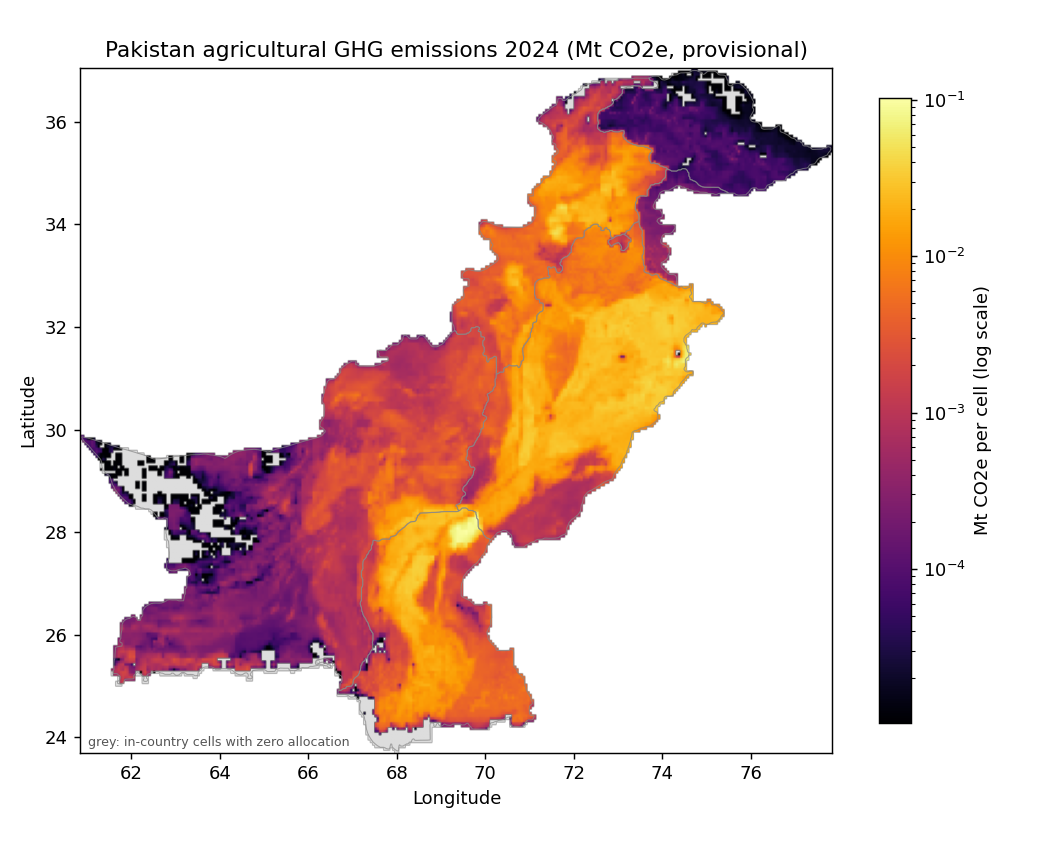
\includegraphics[width=\linewidth]{hotspot_total.png}
\caption{Total agricultural greenhouse-gas emissions on the \SI{0.05}{\degree}
grid in 2024, reported as Mt~\COe{} per cell on a logarithmic scale. The gridded surface
reproduces the provincial and national control totals.}
\label{fig:hotspot}
\end{figure}

\begin{figure*}[!htbp]
\centering
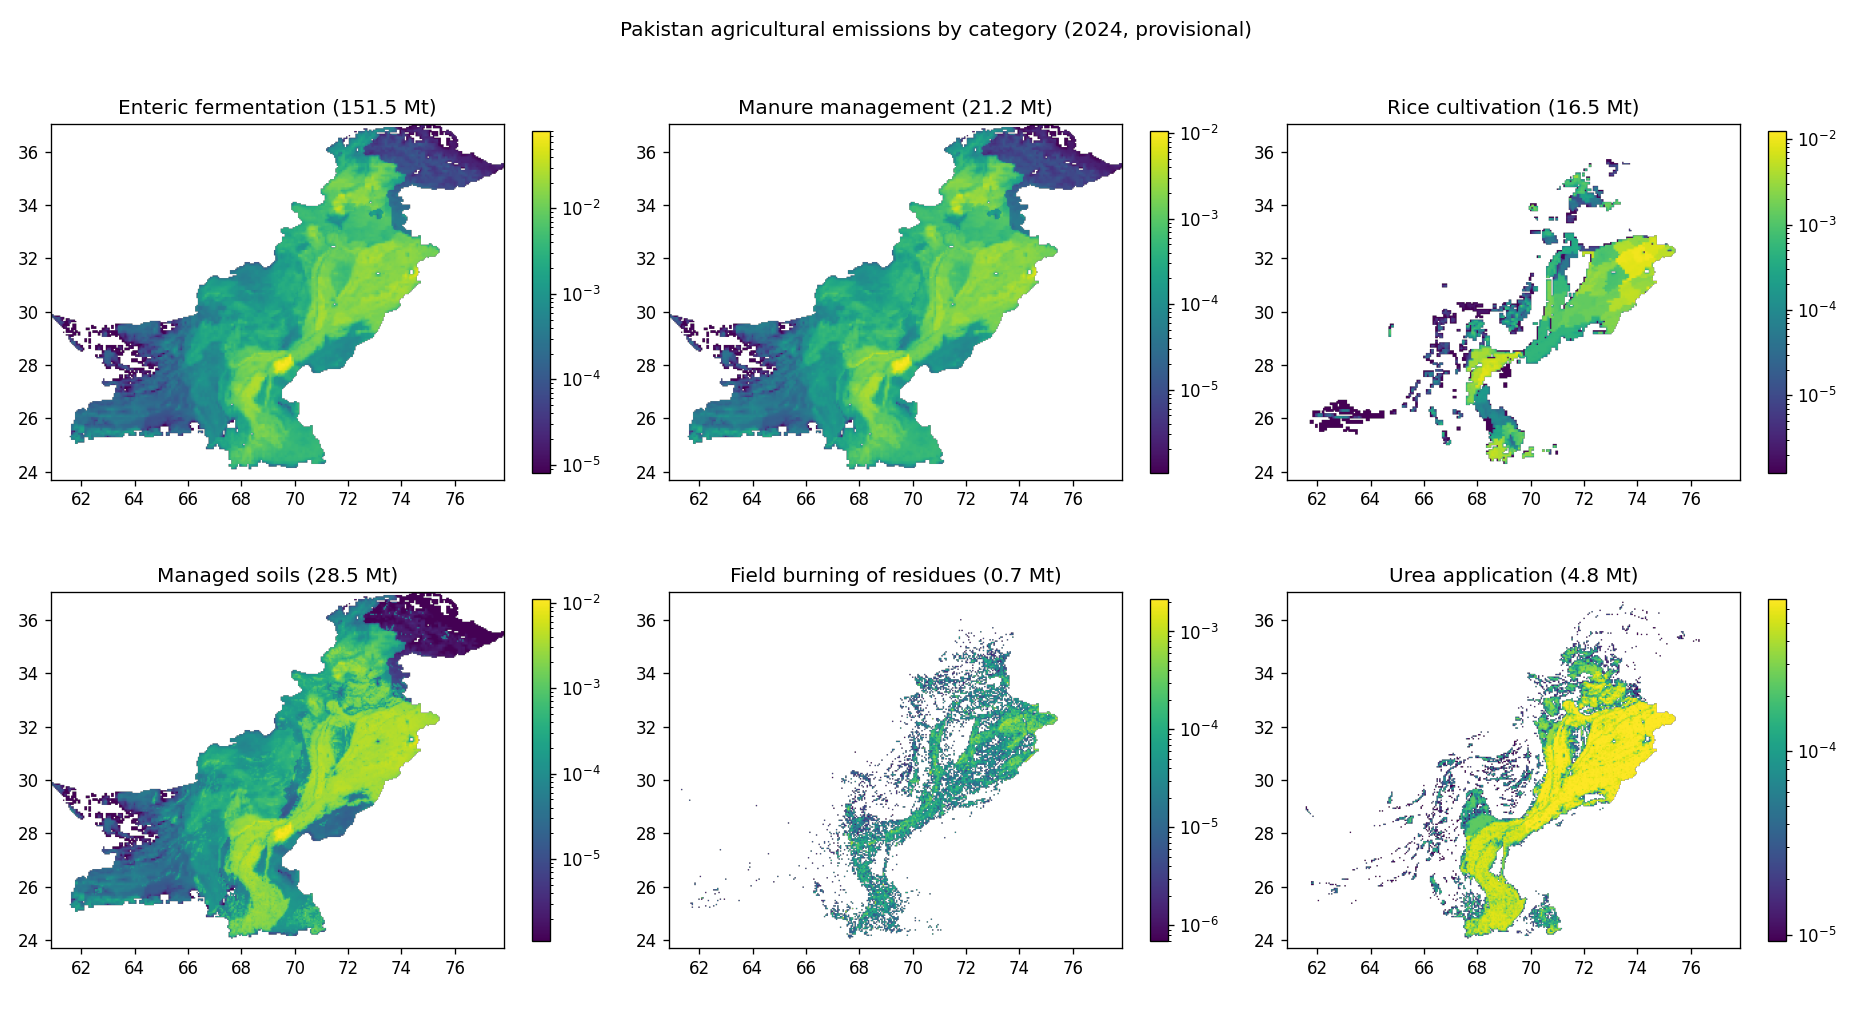
\includegraphics[width=\textwidth]{hotspot_by_category.png}
\caption{Agricultural emissions by category. Livestock emissions follow
species-weighted livestock density, rice methane follows mapped paddy area, and crop-residue
burning follows satellite fire occurrence. Each panel uses its own logarithmic scale; colours
should not be compared directly between categories.}
\label{fig:bycat}
\end{figure*}

\begin{figure}[!htbp]
\centering
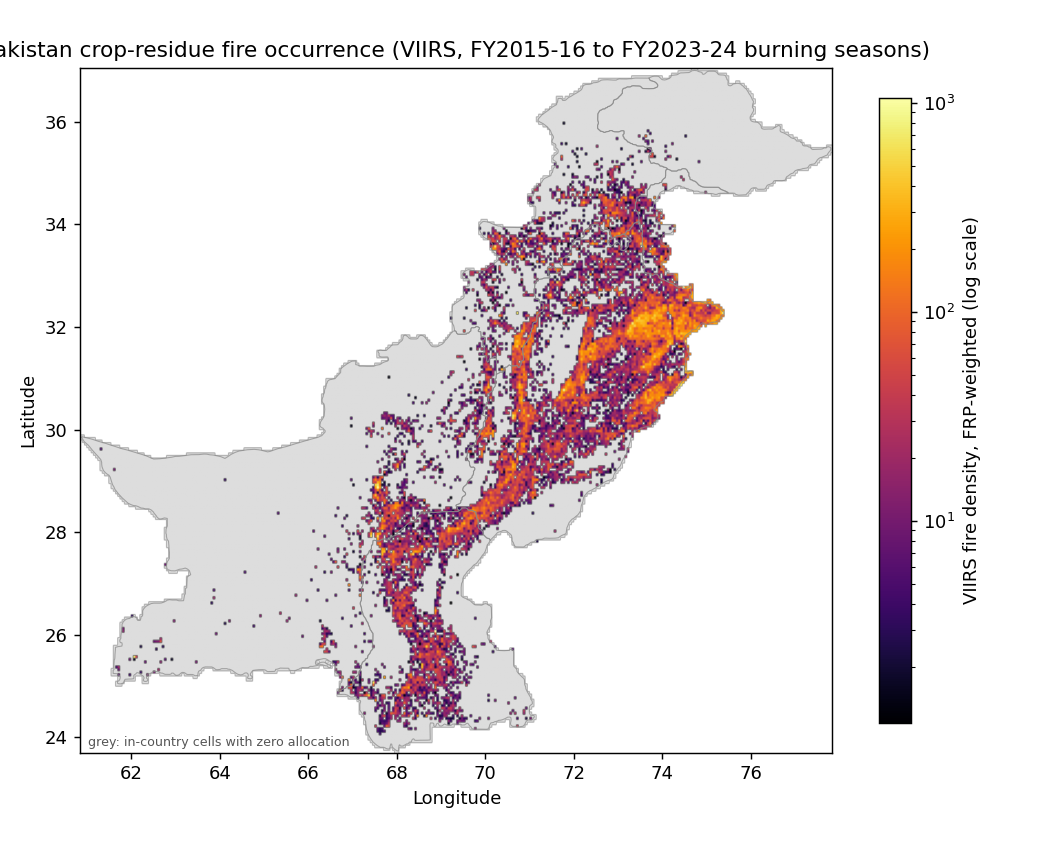
\includegraphics[width=\linewidth]{fire_occurrence.png}
\caption{NASA FIRMS VIIRS active-fire detections used to allocate crop-residue
burning, from the FY2023--24 reporting period's own season: post-monsoon rice-stubble
burning (October--December 2023) and spring wheat-residue burning (April--May 2024),
concentrated mainly in Punjab's rice--wheat belt.}
\label{fig:fire}
\end{figure}

\subsection{District distribution}
\label{sec:results-district}

District allocation resolves the provincial totals to 116 districts and one residual
reporting unit (114 with a boundary polygon, and the two census units---Cholistan Area
and Larkana District---that the boundary file does not draw, carried as named rows on the
province surface)---the four-province base that matches the provincial scope of the
activity statistics, narrower by design than the 134-district census frame the
residential and waste sectors allocate over. This scale corresponds more closely to the
administrative level at which
agricultural and air-quality interventions are commonly implemented.

Most of the highest-emitting districts are located in the central and southern Punjab canal
belt, with one exception at the head of the table. Karachi has the largest estimated total at
\SI{10.18}{}~Mt~\COe{}: the 2024 census enumerates the division's seven districts
separately---\SI{2.8}{} million cattle and \SI{3.6}{} million buffalo, Malir's peri-urban
dairy colonies the largest part---and all seven resolve onto the one Karachi polygon through
the canonical district crosswalk, where earlier releases had placed the shape on the GLW
surface (\SI{0.10}{}~Mt) because none of the seven census names matched it. Jhang follows
at \SI{8.61}{}~Mt~\COe{} and Sheikhupura at \SI{6.73}{}~Mt~\COe{}. Faisalabad and
Muzaffargarh contribute \SI{6.3}{} and \SI{5.8}{}~Mt~\COe{}. The rice-belt
concentration sharpened in this release: rice cultivation now rides the MapSPAM
surface rather than the generic cropland fallback, which lifts the classic
rice districts (Sheikhupura, and Sialkot and Kasur into the table) and is scored
against the Punjab Crop Reporting Service in the spatial benchmarks.

These districts rank highly because they combine large livestock populations, intensively
fertilised cropland and, in some cases, rice production.

Two limits of the district layer are published rather than described, and since rc41 each is
priced as the fraction of every affected stream's own mass that rode the substitute surface,
at that stream's gas and methane origin---earlier releases quoted the whole module mass of the
affected unit, summed across gases without a warming potential. One census unit, Larkana
District, has no polygon of its own in the boundary file, so a stream whose district panel
places mass in it falls back to a within-province spread: the provincial total is unaffected
and the sub-provincial placement of \SI{2.56}{}~Mt~\COe{} across the agriculture,
residential and waste streams is not made. The same class
carries the panel mass of the territories outside the four provinces (ICT, GB, AJK), for which
the district frame has no shapes: \SI{0.35}{}~Mt~\COe{} across agriculture and residential.
In seven shapes the MapSPAM surface shows no paddy at all, so the rice-specific fertiliser
stream is spread uniformly inside them rather than by the declared surface, affecting
\SI{0.029}{}~Mt~\COe{}. All three are listed with their masses and whether they are resolvable in
\texttt{outputs/pakemis\_spatial\_exceptions.csv}. Summing the district layer back over each
province reproduces the provincial allocation exactly
(\texttt{outputs/pakemis\_adm2\_nesting\_check.csv}): each shape's mass is partitioned
among the reporting units of its own province only, so no mass crosses a provincial boundary
between the allocation and the district table.

Matiari in Sindh is the other entry from outside Punjab. Its estimated total
is \SI{4.28}{}~Mt~\COe{} (ninth). Unlike the leading Punjab districts, its total is driven mainly
by livestock density rather than extensive crop cultivation. The category-level
decomposition makes this difference visible.

\begin{table}[!htbp]
\centering
\footnotesize
\begin{tabular}{@{}rllc@{}}
\toprule
\textbf{\#} & \textbf{District} & \textbf{Province} & \textbf{Mt~\COe} \\
\midrule
1  & Karachi           & Sindh  & 10.18 \\
2  & Jhang             & Punjab & 8.61 \\
3  & Sheikhupura       & Punjab & 6.73 \\
4  & Faisalabad        & Punjab & 6.32 \\
5  & Muzaffargarh      & Punjab & 5.84 \\
6  & Dera Ghazi Khan   & Punjab & 4.96 \\
7  & Bahawalnagar      & Punjab & 4.47 \\
8  & Sargodha          & Punjab & 4.43 \\
9  & Matiari           & Sindh  & 4.28 \\
10 & Rahim Yar Khan    & Punjab & 4.14 \\
11 & Okara             & Punjab & 3.98 \\
12 & Bahawalpur        & Punjab & 3.81 \\
13 & Sialkot           & Punjab & 3.74 \\
14 & Kasur             & Punjab & 3.72 \\
15 & Gujranwala        & Punjab & 3.65 \\
\bottomrule
\end{tabular}
\caption{Fifteen districts with the highest total agricultural
greenhouse-gas emissions in 2024, reported in Mt~\COe{} using AR5 GWP-100. District estimates
sum to the provincial and national control totals.}
\label{tab:districttop}
\end{table}

\begin{figure}[!htbp]
\centering
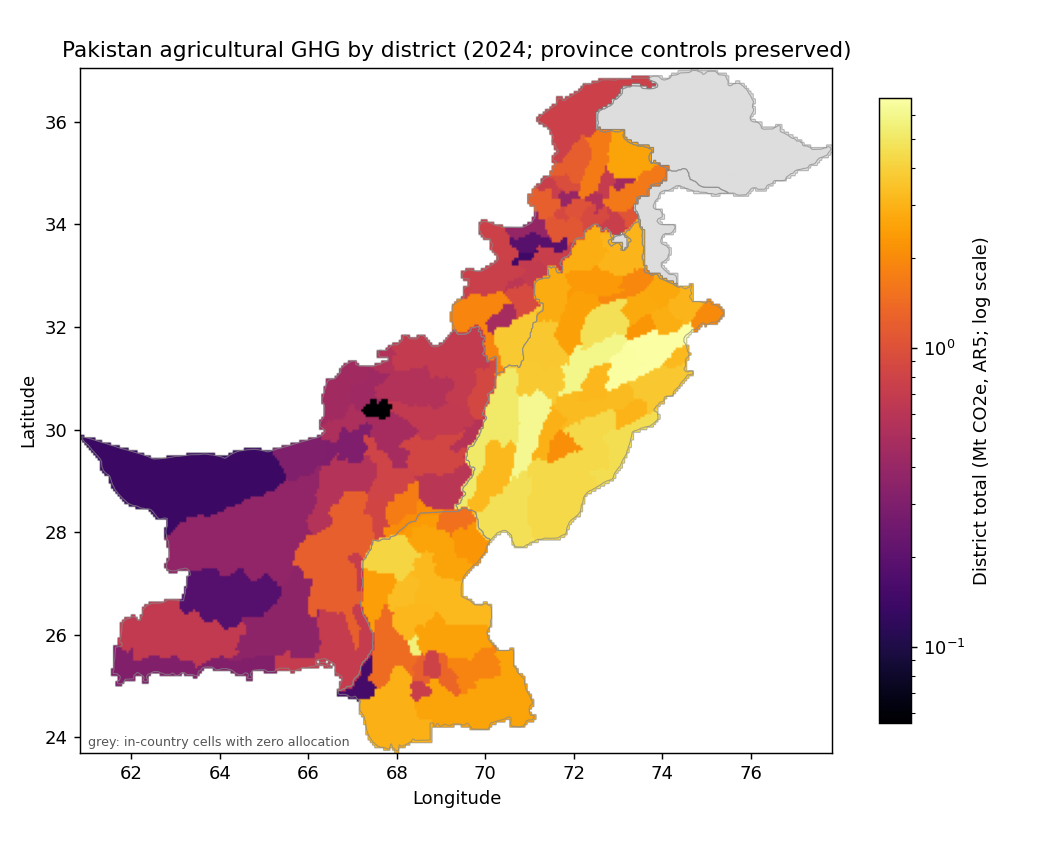
\includegraphics[width=\linewidth]{district_totals.png}
\caption{Agricultural greenhouse-gas emissions by district in 2024. Values
are shown as annual emissions per unit area, allowing districts of different sizes to be
compared. The underlying district totals reproduce the provincial and national inventory.}
\label{fig:districtmap}
\end{figure}

\subsection{National trajectory, 1990--2024}

Agricultural greenhouse-gas emissions increase from approximately \SI{83}{}~Mt~\COe{} in 1990
to \SI{223.5}{}~Mt~\COe{} in 2024. This corresponds to a compound annual growth rate of
approximately \SI{2.9}{\percent}.

The increase is driven mainly by growth in livestock populations and synthetic-fertiliser
use. Emission factors are held constant throughout the series, so the trajectory represents
changes in reported activity rather than changes in methodological assumptions.

The 1990--2023 series uses FAOSTAT activity data on a \emph{calendar-year} basis;
the 2024 value is anchored to the PBS agricultural census and other current
Pakistani sources on the \emph{FY2023--24 fiscal} basis. The join is therefore a
time-basis break as well as a source break---the last FAOSTAT point covers
January--December 2023 while the anchor covers July 2023--June 2024, an overlap of
six months---and the published series carries a \texttt{year\_basis} column
(\texttt{calendar\_faostat} / \texttt{fiscal\_census\_anchor}) so no reader can
treat the two segments as one homogeneous fiscal series. Part of the change between
2023 and 2024 may reflect either transition. This issue is discussed in
Section~\ref{sec:limitations}.

\begin{figure}[!htbp]
\centering
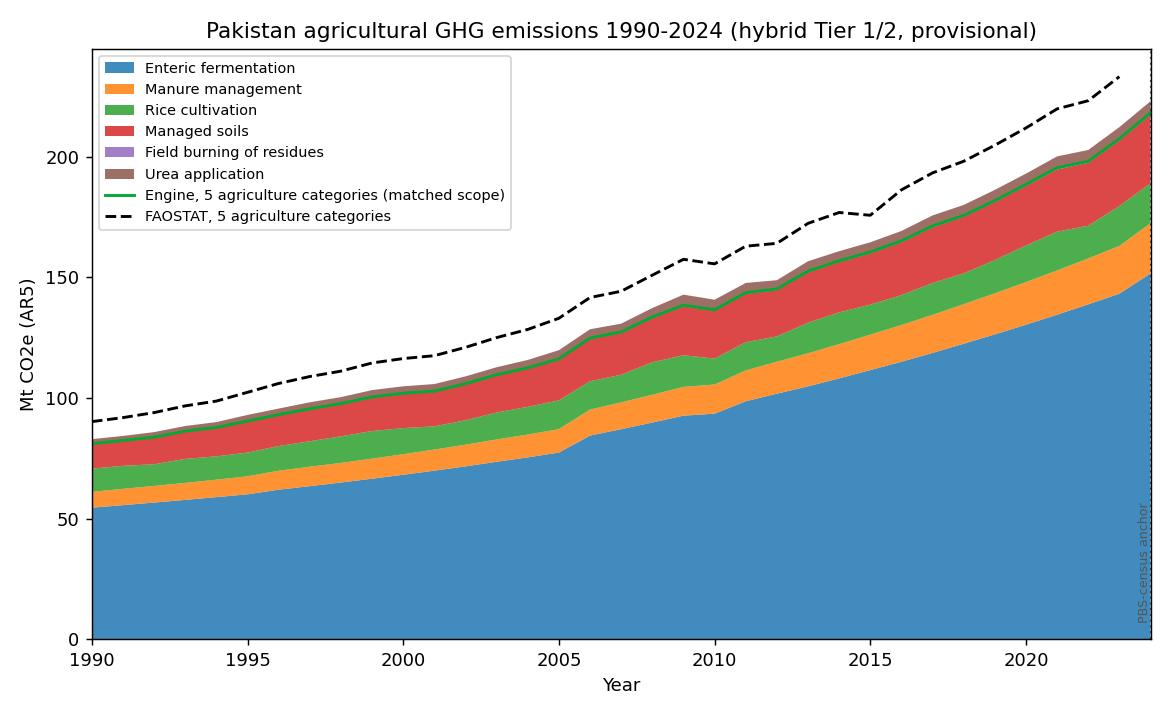
\includegraphics[width=\linewidth]{trend_chart.png}
\caption{Agricultural greenhouse-gas emissions by category, 1990--2024. The
benchmark lines compare this inventory with FAOSTAT using the five categories reported by both
systems. The vertical marker identifies the 2024 transition from the calendar-year FAOSTAT
activity series to the fiscal-year PBS census anchor---a time-basis break as well as
a source break, flagged per row in the published series.}
\label{fig:trend}
\end{figure}

\subsection{Historical district panel}
\label{sec:results-districtyear}

Applying the fixed 2024 district shares to the national time series produces a
district-by-category panel for 1990--2024. The panel contains \num{24290}
district-year-category records and reconciles to the national inventory in every year.

Under the fixed-share assumption, district trajectories follow the national trend.
Sheikhupura increases from approximately \SI{2.9}{}~Mt~\COe{} in 1990 to
\SI{6.7}{}~Mt~\COe{} in 2024. Faisalabad increases from \SI{2.4}{} to \SI{6.6}{}~Mt~\COe{},
and Muzaffargarh from \SI{2.4}{} to \SI{5.8}{}~Mt~\COe{}.

These trajectories should be interpreted as a spatial distribution of the national historical
series. They do not show observed district-specific changes in livestock, cropping patterns
or fertiliser use. Measuring such changes would require consistent historical activity data
at district level. The panel now carries that qualification per row rather than only here:
every record outside the reference year is marked \texttt{reference\_shape\_backcast}, and
only the \num{694} reference-year records are the audited district pattern. A reader who
opens the CSV without this section still cannot mistake a 1990 row for a 1990 observation.

Despite this limitation, the panel provides a district-resolved historical baseline that
remains numerically consistent with the national inventory.

\begin{figure}[!htbp]
\centering
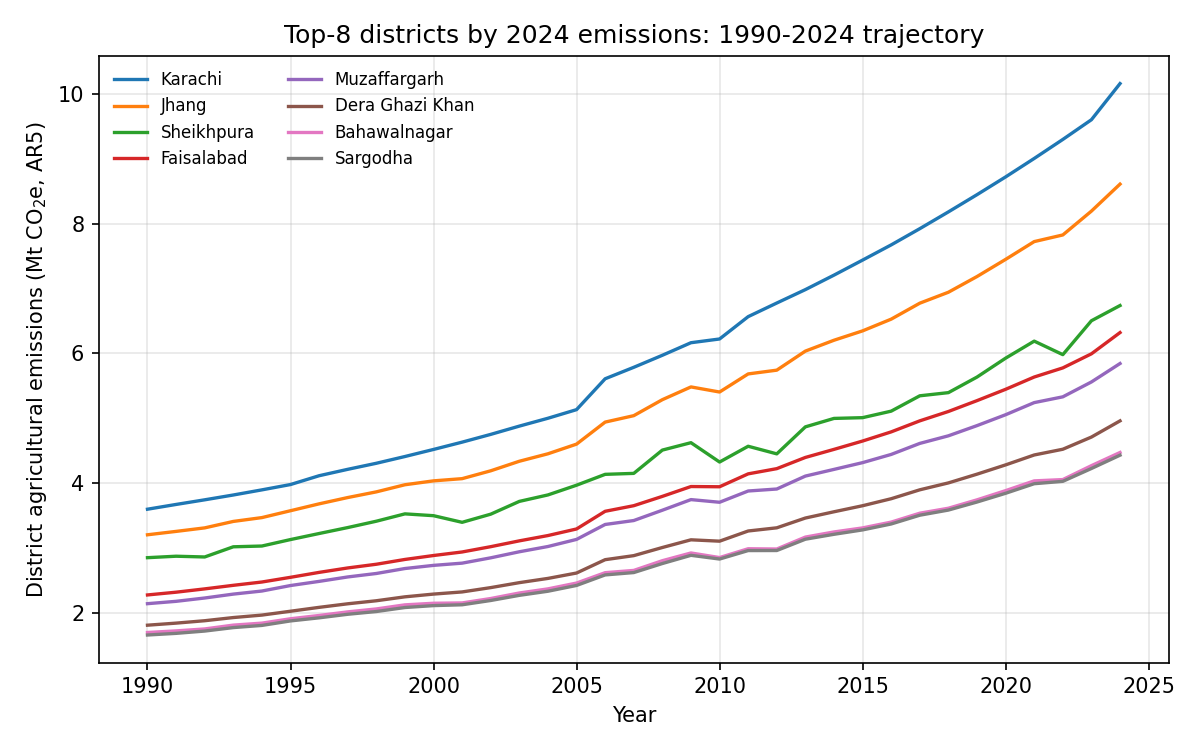
\includegraphics[width=\linewidth]{district_trajectory.png}
\caption{Agricultural greenhouse-gas trajectories for the eight
highest-emitting districts, 1990--2024. District values use fixed 2024 spatial shares and
reproduce the national control total in every year.}
\label{fig:districttraj}
\end{figure}

\subsection{Parametric uncertainty}

The IPCC Approach~1 calculation gives a \SI{95}{\percent} relative half-width of $\pm$19\%
for the national agricultural total.

The Monte-Carlo analysis produces a mean of \SI{223.7}{}~Mt~\COe{}, close to the
deterministic estimate of \SI{223.5}{}~Mt~\COe{}. Its median is \SI{222.3}{}~Mt~\COe{}, and
its \SI{95}{\percent} interval is \SI{185.3}{}--\SI{270.9}{}~Mt~\COe{}. This corresponds to a
relative half-width of approximately \SI{19.2}{\percent}.

The close agreement indicates that the national interval is not highly sensitive to whether
the documented uncertainties are propagated analytically or through mean-preserving lognormal
sampling. Both calculations use the same underlying assumptions and the correlation treatment
described in Section~\ref{sec:methods}.

Rice cultivation has the widest category-level uncertainty at $\pm$62\%, reflecting
uncertainty in cultivation conditions and the assumed water regime. Managed soils follow at
$\pm$47\%, largely because of uncertainty in direct and indirect \NtwoO{} factors. Urea
application has the narrowest interval at $\pm$11\%.

These results show that improved information on rice water management and soil \NtwoO{}
factors would reduce national inventory uncertainty more than further refinement of the urea
calculation.

\begin{table*}[!htbp]
\centering
\footnotesize
\begin{tabular}{@{}lccccc@{}}
\toprule
\textbf{Category} & \textbf{Mean} & \textbf{P2.5} & \textbf{P50} & \textbf{P97.5}
& \textbf{$\pm$\%} \\
\midrule
Enteric fermentation & 151.9 & 117.9 & 150.7 & 194.3 & 25 \\
Manure management    &  21.2 &  15.8 &  20.7 &  29.8 & 33 \\
Managed soils        &  28.5 &  17.9 &  27.5 &  44.5 & 47 \\
Rice cultivation     &  16.6 &   8.7 &  15.8 &  28.6 & 61 \\
Urea application     &   4.8 &   4.3 &   4.8 &   5.4 & 11 \\
Field burning        &   0.7 &   0.4 &   0.7 &   1.0 & 45 \\
\midrule
\textbf{Total}       & \textbf{223.7} & \textbf{185.3} & \textbf{222.3} & \textbf{270.9}
& \textbf{19} \\
\bottomrule
\end{tabular}
\caption{Monte-Carlo means, medians and \SI{95}{\percent} intervals for the national
agricultural inventory, together with the IPCC Approach~1 \SI{95}{\percent} relative
half-width. Both approaches use the same activity-data and emission-factor uncertainties.}
\label{tab:mc}
\end{table*}

\begin{figure}[!htbp]
\centering
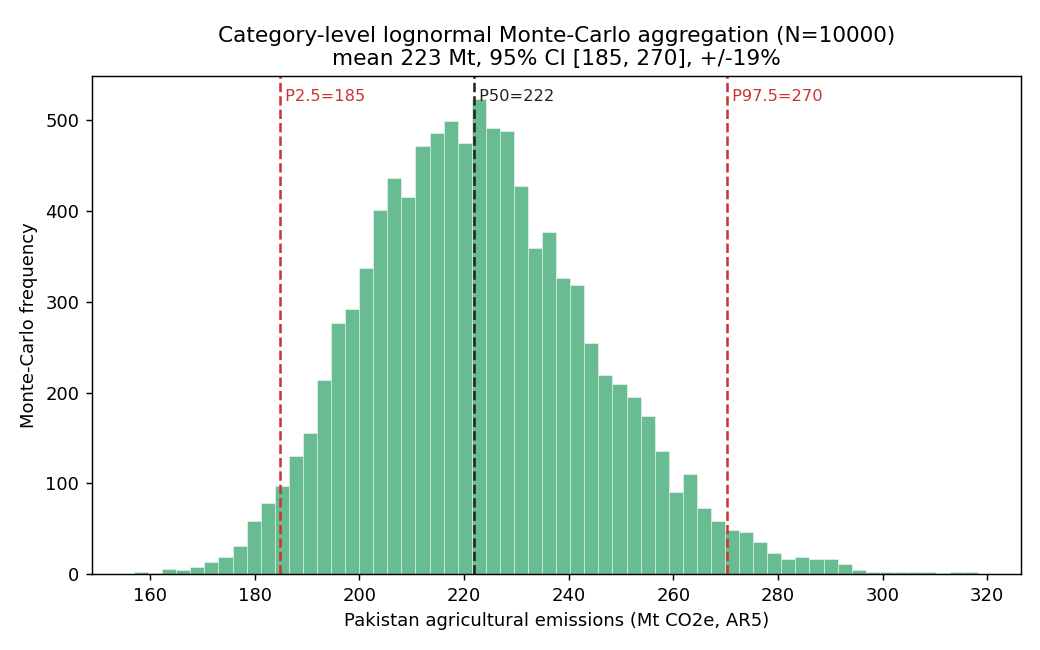
\includegraphics[width=\linewidth]{uncertainty_distribution.png}
\caption{Monte-Carlo distribution of total agricultural greenhouse-gas emissions
based on \num{10000} draws. The figure marks the median and the 2.5th and 97.5th
percentiles.}
\label{fig:uncert}
\end{figure}

\subsection{Key categories}

Four categories qualify as key under the IPCC Approach~1 level or trend assessment: enteric
fermentation, managed soils, manure management and rice cultivation. Together they account
for more than \SI{95}{\percent} of both the 2024 inventory level and the contribution to the
1990--2024 trend.

Enteric fermentation dominates the level assessment, contributing \SI{67.9}{\percent} of the
2024 total. Rice cultivation contributes only \SI{7.4}{\percent} of the 2024 level but
accounts for \SI{48.6}{\percent} of the trend assessment.

The trend result does not mean that rice emissions grew faster than the other categories.
Rice emissions increased by a factor of approximately \num{1.7} between 1990 and 2024,
compared with factors of \num{2.7}--\num{3.2} for the other major categories. Rice ranks
highly because its slower growth caused its share of the inventory to change substantially
relative to the sector average.

The four key categories include those with the widest uncertainty bands, particularly rice
cultivation and managed soils. They are therefore the highest-priority categories for
improved activity data and country-specific Tier~2 or Tier~3 emission factors.

\begin{table}[!htbp]
\centering
\footnotesize
\begin{tabular}{@{}lccc@{}}
\toprule
\textbf{Category} & \textbf{Level \%} & \textbf{Trend \%} & \textbf{Key} \\
\midrule
Enteric fermentation & 67.9 & 27.3 & \checkmark \\
Managed soils        & 12.8 &  5.0 & \checkmark \\
Manure management    &  9.5 & 17.7 & \checkmark \\
Rice cultivation     &  7.4 & 48.6 & \checkmark \\
Urea application     &  2.2 &  1.2 & \\
Field burning        &  0.3 &  0.1 & \\
\bottomrule
\end{tabular}
\caption{IPCC Approach~1 key-category assessment for agriculture. The level
assessment reports each category's share of the 2024 total. The trend assessment measures its
contribution to the change in inventory composition between 1990 and 2024. A category is
classified as key if it falls within the cumulative \SI{95}{\percent} threshold under either
assessment.}
\label{tab:keycat}
\end{table}

\subsection{Effect of correcting the livestock nitrogen boundaries}
\label{sec:results-nledger}

The shared nitrogen ledger was used to align the greenhouse-gas and air-pollutant
calculations.

Before alignment, the greenhouse-gas calculation appeared to indicate that \SI{21}{\percent}
of managed nitrogen volatilised, compared with \SI{49.5}{\percent} in the air-pollutant
calculation. This apparent difference resulted largely from comparing different stages and
chemical bases. The IPCC fractions represented both \NHthree{}-N and \NOx{}-N and separated
pre-field losses from post-application losses, whereas the EMEP/EEA calculation represented
\NHthree{}-N and followed the complete stage sequence from housing through storage and field
application.

After conversion to a common \NHthree{}-N basis, the total livestock volatilisation estimates
are relatively close. The IPCC chain gives \SI{1.967}{}~Mt \NHthree{}-N, while the EMEP/EEA
chain gives \SI{1.588}{}~Mt \NHthree{}-N. The ratio is \num{1.24}.

The stage-level comparison is less consistent. Housing and storage differ by a factor of
\num{1.25}. The IPCC field-application estimate is \num{0.65} times the EMEP/EEA value, while
the IPCC grazing estimate is \num{3.53} times the EMEP/EEA value. The similar aggregate
totals therefore result partly from offsetting stage-level differences.

The greenhouse-gas inventory retains the IPCC nitrogen-accounting chain because the inventory
is reported under IPCC methods. The air-pollutant calculation retains the EMEP/EEA
stage-resolved method because ammonia losses must be assigned to housing, storage, grazing
and field application. Replacing the IPCC loss formulation with the EMEP/EEA formulation in
the greenhouse-gas pathway would change the national total by only approximately
\SI{0.24}{}~Mt~\COe{}. The choice of representation is therefore based mainly on
methodological scope rather than on its effect on the headline total.

Correcting the earlier IPCC nitrogen chain reduced the quantity of manure nitrogen reaching
soils from \SI{2.72}{} to \SI{2.33}{}~Mt~N. This lowered the agricultural greenhouse-gas
total by \SI{0.62}{}~Mt~\COe{}, from \SI{221.71}{} to \SI{221.09}{}~Mt~\COe{}. A subsequent
update to the synthetic-fertiliser factor produced \SI{221.2}{}~Mt~\COe{}; the
harmonisation round's activity refresh and the rc39 herd re-base then carried the published
total to \SI{223.5}{}~Mt~\COe{}. Supplementary Note~S5 documents the corrections.

The correction does not change livestock \NHthree{}, because the air-pollutant module reads
the managed and grazing nitrogen pools directly rather than deriving ammonia from the final
manure-applied pool.

The common ledger guarantees that the same nitrogen is not assigned to multiple stages or
omitted between them. It does not require the IPCC and EMEP/EEA methods to produce identical
volatilised masses within each stage.

\begin{table}[!htbp]
\centering
\footnotesize
\begin{tabular}{@{}lrr@{}}
\toprule
\textbf{Flow} & \textbf{Mt N} & \textbf{\% excreted} \\
\midrule
\multicolumn{3}{@{}l}{\emph{A. Excretion partition}} \\
Total N excreted                          & 7.78 & 100.0 \\
\quad to grazing ($F_{PRP}$)                & 3.18 & 40.9 \\
\quad to managed systems                  & 3.34 & 42.9 \\
\quad diverted as dung-cake fuel (to Energy) & 1.26 & 16.2 \\
\midrule
\multicolumn{3}{@{}l}{\emph{B. Pre-field management (Eq.~10.34a)}} \\
\NHthree{}-N + \NOx{}-N ($\mathrm{Frac_{GasMS}}$) & 0.91 & 11.7 \\
leaching, N\textsubscript{2}, and \NtwoO{}-N          & 0.09 &  1.2 \\
\quad = N available for application ($F_{ON}$) & 2.33 & 30.0 \\
\midrule
\multicolumn{3}{@{}l}{\emph{C. Field application, gross basis (Ch.~11)}} \\
direct soil \NtwoO{}-N ($EF_1$)           & 0.01 &  0.1 \\
\NHthree{}-N + \NOx{}-N ($\mathrm{Frac_{GASM}}$) & 0.49 &  6.3 \\
leaching/run-off                          & 0.45 &  5.8 \\
\quad = retained in the soil nitrogen pool & 1.38 & 17.8 \\
\midrule
\multicolumn{3}{@{}l}{\emph{Same managed pool on the EMEP/EEA TAN basis}} \\
housing, yards and storage \NHthree{}-N   & 0.69 &  8.9 \\
field-application \NHthree{}-N            & 0.71 &  9.2 \\
\bottomrule
\end{tabular}
\caption{National livestock nitrogen ledger for 2024. The IPCC chain tracks
excreted nitrogen through grazing, managed systems, pre-field losses, field application,
leaching and retention in soils. The EMEP/EEA rows provide a parallel TAN-based representation
of ammonia losses from the same managed nitrogen pool.
Generated by
\texttt{src/pkinv/sectors/agriculture/n\_ledger.py}.}
\label{tab:nledger}
\end{table}

\begin{table}[!htbp]
\centering
\footnotesize
\begin{tabular}{@{}lrrr@{}}
\toprule
\textbf{Stage} & \textbf{IPCC} & \textbf{EMEP} & \textbf{Ratio} \\
\midrule
Housing + storage   & 0.866 & 0.694 & 1.25 \\
Field application   & 0.466 & 0.714 & \textbf{0.65} \\
Grazing             & 0.635 & 0.180 & \textbf{3.53} \\
\midrule
\textbf{Total}      & \textbf{1.967} & \textbf{1.588} & \textbf{1.24} \\
\bottomrule
\end{tabular}
\caption{Livestock ammonia losses by stage after conversion to a common
\NHthree{}-N basis. The IPCC and EMEP/EEA totals are similar, but field-application and grazing
estimates differ substantially in opposite directions.
Generated by \texttt{src/pkinv/sectors/agriculture/n\_ledger.py}.}
\label{tab:stages}
\end{table}

\FloatBarrier
% ===========================================================================
\section{Agricultural Air-Pollutant Co-emissions}
\label{sec:airpollutants}
% ===========================================================================

Agriculture is a major source of ammonia in South Asia. Crop-residue burning also produces
particulate matter and combustion gases that contribute to seasonal air-pollution episodes.

The air-pollutant inventory reports emissions in native mass units rather than converting
them to \COe{}. The calculation methods and nitrogen accounting are described in
Section~\ref{sec:methods-shared}; this section reports the resulting national, spatial,
historical and benchmark estimates.

The air-pollutant layer follows the same general processing framework as the greenhouse-gas
inventory. Emissions are calculated nationally and allocated to provinces, a
\SI{0.05}{\degree} grid and 116 districts using stream-specific spatial proxies. National
time series are reconstructed for 1990--2024, and parametric uncertainty is evaluated
analytically and by Monte-Carlo simulation.

The two layers differ in the status of their national totals. The greenhouse-gas total is
calculated within the formal IPCC inventory structure. The air-pollutant totals are bottom-up
estimates developed in this study. They therefore serve as separate control totals for the
air-pollutant spatial products and require external evaluation.

Each air-pollutant grid, district table and provincial allocation reproduces its
corresponding national pollutant total to a relative numerical residual below $10^{-9}$.

\subsection{National air-pollutant totals}

Agricultural \NHthree{} emissions in 2024 are estimated at \SI{2.67}{}~Mt.

Housing, yards and manure storage contribute approximately \SI{0.84}{}~Mt. Manure applied to
agricultural soils contributes a further \SI{0.87}{}~Mt. Synthetic fertiliser contributes
\SI{0.74}{}~Mt, and grazing deposition contributes approximately \SI{0.22}{}~Mt.
Crop-residue burning adds approximately \SI{9}{}~kt.

Crop-residue burning also produces an estimated \SI{654}{}~kt of CO, \SI{54}{}~kt of
PM$_{2.5}$, \SI{50}{}~kt of NMVOC, \SI{18}{}~kt of \NOx{}, \SI{3.6}{}~kt of black carbon and
\SI{2.8}{}~kt of SO$_2$. Agricultural soil processes contribute an additional \SI{145}{}~kt
of \NOx{}, bringing total agricultural \NOx{} emissions to approximately \SI{163}{}~kt.

Punjab contributes \SI{1.53}{}~Mt of \NHthree{}, followed by Sindh at \SI{0.61}{}~Mt, Khyber
Pakhtunkhwa at \SI{0.28}{}~Mt and Balochistan at \SI{0.26}{}~Mt.

The provincial pattern reflects the combination of fertilised cropland and livestock
production. Manure-application \NHthree{} is particularly sensitive to the spatial treatment
because it occurs neither strictly where manure is produced nor uniformly across cropland; it
is allocated using the intersection of livestock density and cropland.

\begin{table*}[!htbp]
\centering
\footnotesize
\begin{tabular}{@{}lrrrrrrr@{}}
\toprule
\textbf{Category (kt)} & \textbf{\NHthree{}} & \textbf{\NOx{}} & \textbf{PM$_{2.5}$}
& \textbf{CO} & \textbf{NMVOC} & \textbf{BC$^{a}$} & \textbf{SO$_2$} \\
\midrule
Managed soils      & 1822 & 145 & --- & --- & --- & --- & --- \\
Manure management  &  843 & --- & --- & --- & --- & --- & --- \\
Field burning      &    9 &  18 &  54 & 654 &  50 & 3.6 & 2.8 \\
\midrule
\textbf{Total}     & \textbf{2675} & \textbf{163} & \textbf{54} & \textbf{654}
& \textbf{50} & \textbf{3.6} & \textbf{2.8} \\
\bottomrule
\end{tabular}
\caption{Agricultural air-pollutant emissions in 2024, reported in kt of
native pollutant mass. Black carbon is included within PM$_{2.5}$ and should not be added to
it. \NOx{} is reported as NO$_2$-equivalent mass. The air-pollutant values define separate
national controls and are not components of the greenhouse-gas \COe{} total.
$^{a}$Black carbon is a \emph{component} of PM$_{2.5}$, not additive to
it. \NOx{} is reported as NO$_2$-equivalent mass. ``Managed soils''
\NHthree{} comprises synthetic fertiliser, manure applied to soils and grazing
deposition. Uncertainties are given per pollutant in Table~\ref{tab:apunc} and per
factor in Table~\ref{tab:apef}. Not part of the GHG control-total reconciliation.}
\label{tab:apresults}
\end{table*}

\subsection{Spatial distribution}
\label{sec:ap-spatial}

Each pollutant stream is allocated using the same dasymetric equation applied to the
greenhouse-gas inventory.

\NHthree{} from livestock housing, yards, storage and grazing follows gridded livestock
density. At district level, census head-counts replace the gridded proxy where suitable
matches are available.

\NHthree{} from manure application follows cropland weighted by livestock density.
Synthetic-fertiliser \NHthree{} follows cropland, with rice-specific nitrogen allocated to
mapped paddy area. Pollutants from residue burning follow satellite active-fire detections.

This common proxy framework keeps the greenhouse-gas and air-pollutant products spatially
consistent for nitrogen streams derived from the same activity.

Ammonia emissions are concentrated in the canal-belt and livestock-producing districts.
Jhang has the highest district estimate at approximately \SI{93}{}~kt, followed by
Muzaffargarh at \SI{85}{}~kt, Sheikhupura at \SI{83}{}~kt, Sargodha at \SI{75}{}~kt and
Rahim Yar Khan at \SI{66}{}~kt.

Karachi---the one polygon that receives the division's seven census districts, Malir's
peri-urban dairy colonies the largest part---again represents a livestock-dominated profile,
whereas the leading Punjab districts combine livestock and intensive cultivation.

\begin{figure}[!htbp]
\centering
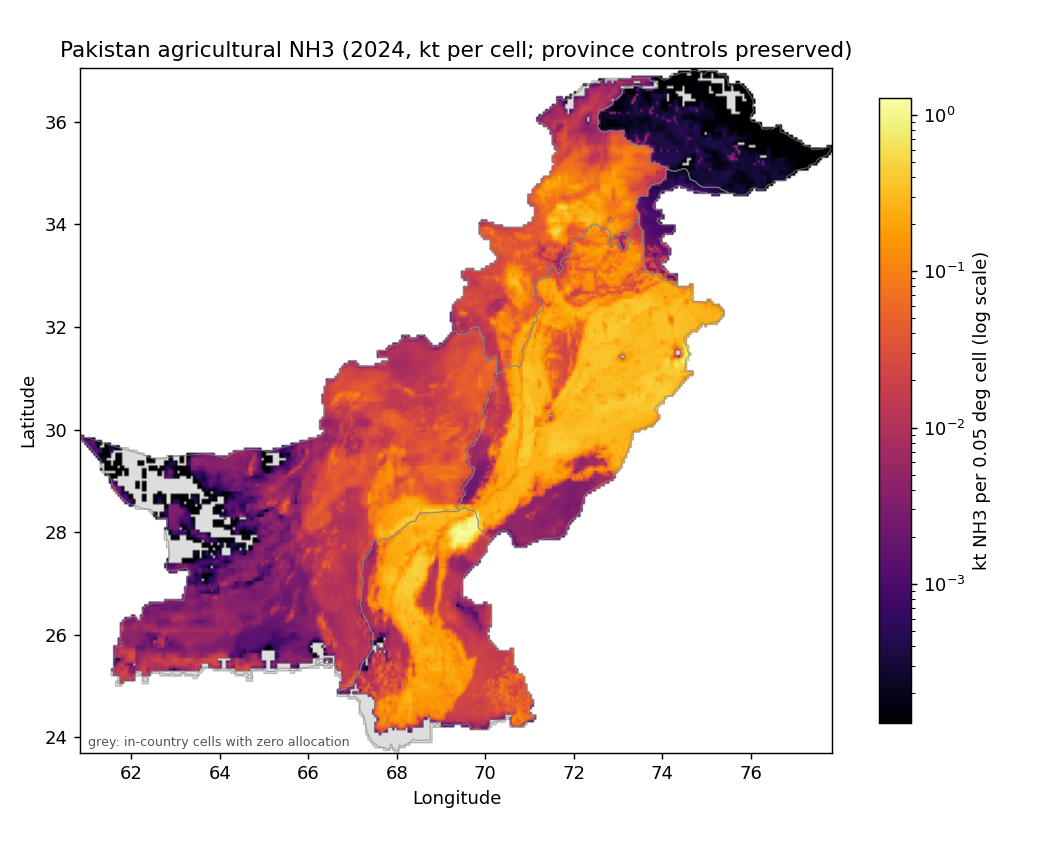
\includegraphics[width=\linewidth]{nh3_map.png}
\caption{Agricultural \NHthree{} emissions on the \SI{0.05}{\degree} grid in
2024, reported as kt \NHthree{} per cell on a logarithmic scale. Each nitrogen stream is
allocated using its process-specific spatial proxy, and the combined surface reproduces the
provincial and national air-pollutant totals.}
\label{fig:nh3map}
\end{figure}

\subsection{Historical trajectory}
\label{sec:ap-timeseries}

Agricultural \NHthree{} emissions increase from approximately \SI{784}{}~kt in 1990 to
\SI{2675}{}~kt in 2024, a factor of \num{3.4}.

The increase reflects growth in livestock populations and synthetic-fertiliser use. Emission
factors remain fixed throughout the series, so changes represent the historical activity
data.

CO from crop-residue burning increases from approximately \SI{250}{}~kt to \SI{654}{}~kt, a
factor of \num{2.6}. The remaining crop-burning pollutants follow the same underlying change
in burned dry matter.

As in the greenhouse-gas reconstruction, the 1990--2023 estimates use FAOSTAT activity data,
while 2024 is anchored to the PBS census and current Pakistani statistics. The difference in
crop coverage at this transition is discussed in Section~\ref{sec:limitations}.

\begin{figure}[!htbp]
\centering
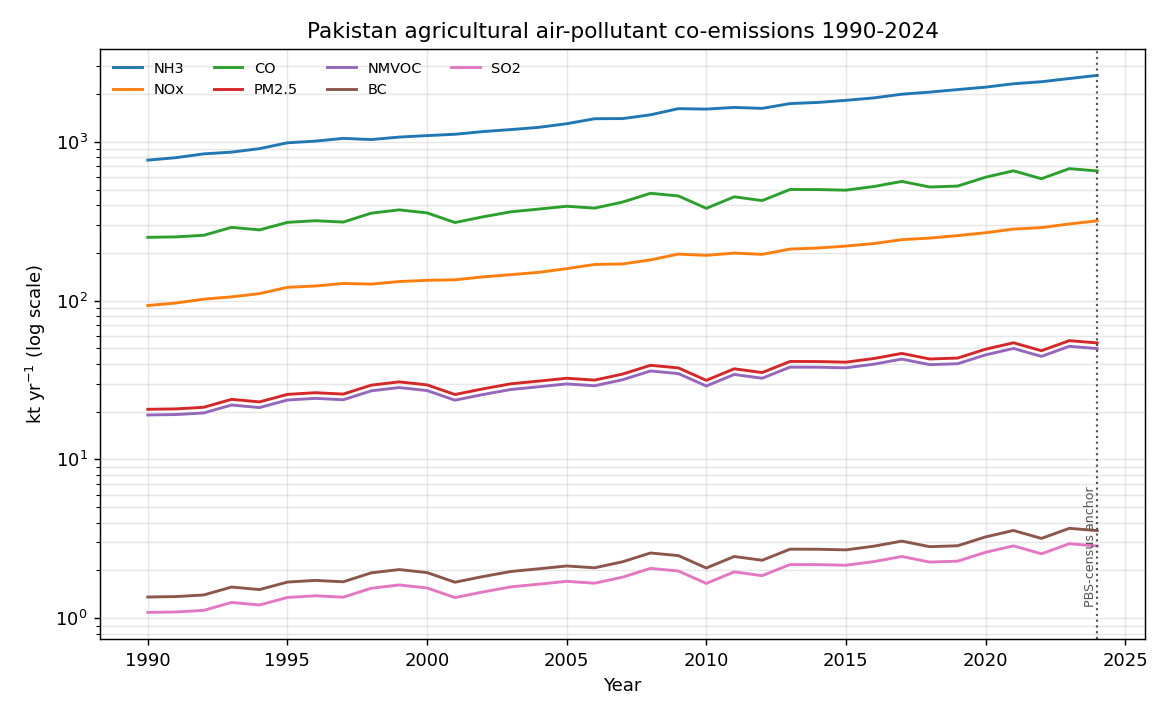
\includegraphics[width=\linewidth]{air_trend.png}
\caption{Agricultural air-pollutant emissions, 1990--2024, reported in kt on a
logarithmic scale. The vertical marker identifies the 2024 transition from the FAOSTAT
activity series to the PBS census anchor.}
\label{fig:airtrend}
\end{figure}

\subsection{Parametric uncertainty and key sources}

Air-pollutant uncertainty is propagated using the same analytical and Monte-Carlo procedures
as the greenhouse-gas inventory.

The Monte-Carlo analysis gives a mean \NHthree{} estimate of \SI{2676}{}~kt and a
\SI{95}{\percent} interval of \SI{2120}{}--\SI{3359}{}~kt. The corresponding Approach~1
relative half-width is $\pm$24\%.

Among the reported pollutants, \NHthree{} has the narrowest parametric relative interval.
Soil and fertiliser \NOx{} have the widest combined uncertainty at $\pm$90\%. Crop-burning
uncertainties range from $\pm$54\% for CO to $\pm$79\% for SO$_2$.

The comparatively narrow \NHthree{} parametric interval does not include uncertainty in the
national manure-management distribution. That structural uncertainty is evaluated separately
in Section~\ref{sec:ap-structural}.

Four sources qualify as key for \NHthree{}: manure applied to soils, contributing
approximately \SI{32}{\percent}; livestock housing and storage, contributing
\SI{32}{\percent}; synthetic fertiliser, contributing \SI{28}{\percent}; and small-ruminant
grazing, contributing \SI{4}{\percent}. Together these sources exceed the cumulative
\SI{95}{\percent} threshold. The \emph{ordering} of the three leading sources is soft, and
the published ranking now says so quantitatively: under the per-source Monte Carlo their
level shares overlap almost completely (each spanning roughly 20--44\%), and each holds its
point-estimate rank in only about a third to a half of draws
(\texttt{rank\_stability\_pct} in \texttt{outputs/air\_key\_categories.csv}). The key-source
\emph{set} is stable; which of the three leads is not resolvable at the current
uncertainties. Each of the remaining pollutants is dominated by crop-residue burning, so
residue burning is its principal key source---at \SI{100}{\percent} of the pollutant's
total, a statement about coverage (no other stream is estimated) rather than certainty,
as the table's note column records.

\begin{table*}[!htbp]
\centering
\footnotesize
\begin{tabular}{@{}lrrrrr@{}}
\toprule
\textbf{Pollutant} & \textbf{Mean} & \textbf{P2.5} & \textbf{P50} & \textbf{P97.5}
& \textbf{$\pm$\%} \\
\midrule
\NHthree{}   & 2676 & 2120 & 2657 & 3359 & 23 \\
\NOx{}       &  163 &   67 &  148 &  349 & 90 \\
CO           &  653 &  376 &  628 & 1074 & 54 \\
PM$_{2.5}$   &   54 &   28 &   52 &   94 & 62 \\
NMVOC        &   50 &   24 &   47 &   93 & 70 \\
BC           &  3.5 &  1.7 &  3.4 &  6.6 & 70 \\
SO$_2$       &  2.8 &  1.2 &  2.6 &  5.6 & 79 \\
\bottomrule
\end{tabular}
\caption{Monte-Carlo means and \SI{95}{\percent} intervals for agricultural air
pollutants, together with IPCC Approach~1 relative half-widths. The estimates include
parameter and activity-data uncertainty under the reference manure-management configuration
but exclude structural uncertainty among alternative management configurations.}
\label{tab:apunc}
\end{table*}

\subsection{Inventory scope and completeness}
\label{sec:ap-completeness}

The air-pollutant inventory distinguishes estimated sources, known unestimated sources, and
sources outside the agricultural activity basis. Three reporting conventions are important.

First, black carbon is a component of PM$_{2.5}$ and must not be added to the PM$_{2.5}$
estimate. Second, \NOx{} is reported as NO$_2$-equivalent mass, a convention that differs
from the underlying nitrogen or NO mass used in parts of the calculation. Third, the
inventory estimates emissions. It does not estimate ambient concentrations, population
exposure or health effects, and no atmospheric transport or chemistry model is applied in
this study.

Agricultural machinery and tillage or harvest dust are the main declared source gaps.
Suitable activity data and methods for these sources are not included in the present system.

\begin{table*}[!htbp]
\centering
\footnotesize
\begin{tabular}{@{}lccccccc@{}}
\toprule
\textbf{Source} & \textbf{\NHthree{}} & \textbf{\NOx{}} & \textbf{PM$_{2.5}$}
& \textbf{PM$_{10}$} & \textbf{CO} & \textbf{NMVOC} & \textbf{SO$_2$} \\
\midrule
Livestock housing and storage & E  & NE & NE & NE & --- & NE & --- \\
Grazing deposition            & E  & NE & --- & --- & --- & --- & --- \\
Manure application            & E  & E$^{a}$ & --- & --- & --- & --- & --- \\
Synthetic fertiliser          & E  & E  & --- & --- & --- & --- & --- \\
Residues left in field        & E$^{b}$ & NE & --- & --- & --- & --- & --- \\
Residue burning               & E  & E  & E  & NE & E  & E  & E \\
Agricultural machinery        & NE & NE & NE & NE & NE & NE & NE \\
Tillage and harvest dust      & --- & --- & NE & NE & --- & --- & --- \\
\bottomrule
\end{tabular}
\caption{Completeness assessment for agricultural air pollutants.
``Estimated'' indicates sources quantified in this inventory, ``not estimated'' identifies
known sources outside the current calculation, and a dash indicates that the
source--pollutant combination is not applicable. Black carbon is included within
PM$_{2.5}$.
$^{a}$Included in the soil \NOx{} term, which is parameterised on total
applied nitrogen rather than per source. $^{b}$Estimated as a computed zero
(Section~\ref{sec:ap-scope}). Black carbon (estimated for residue burning) is a component of
PM$_{2.5}$, not additive to it. Agricultural machinery and tillage dust are outside this
inventory's activity basis and are the largest declared gaps.}
\label{tab:apcompleteness}
\end{table*}

\subsection{Spatial-proxy crosswalk}
\label{sec:ap-crosswalk}

Table~\ref{tab:crosswalk} summarises the spatial proxy used for each emission stream at
provincial, gridded and district levels.

Livestock housing and storage use livestock shares at provincial level, \GLW{} density on the
grid, and PBS census head-counts at district level. Grazing uses the same broad livestock
basis, with species distinctions retained where relevant.

Applied manure uses the cropland--livestock intersection. Synthetic fertiliser uses provincial
offtake, cropland on the grid, and district cropland, except for the rice-specific stream,
which uses rice area at each scale.

Crop residues retained in fields use crop production and cropland proxies. Residue-burning
pollutants use crop production for provincial controls and FIRMS active-fire detections for
grid and district allocation.

Using one crosswalk for the greenhouse-gas and air-pollutant modules prevents corresponding
nitrogen streams from being assigned incompatible spatial proxies.

\begin{table*}[!htbp]
\centering
\footnotesize
\begin{tabular}{@{}llll@{}}
\toprule
\textbf{Emission stream} & \textbf{Province} & \textbf{Grid} & \textbf{District} \\
\midrule
Housing/storage \NHthree{}, manure \CHfour{}/\NtwoO{} & livestock & \GLW{} density & PBS census heads \\
Grazing \NHthree{}, pasture \NtwoO{} & livestock (small rum.\ split) & \GLW{} density & PBS census heads \\
Applied-manure \NHthree{}/\NtwoO{} & manure-applied & cropland $\times$ \GLW{} & census $\times$ cropland \\
Synthetic fertiliser, upland & fertiliser offtake & cropland & district cropland \\
Synthetic fertiliser, rice & rice area & MapSPAM rice (held, hash-pinned) & official rice area \\
Crop residues (returned) & crop production & cropland & district cropland \\
Residue burning, all pollutants & crop production & FIRMS active fire & FIRMS active fire \\
Urea \COtwo{} & fertiliser offtake & cropland & district cropland \\
\bottomrule
\end{tabular}
\caption{Spatial proxies used for greenhouse-gas and air-pollutant emission
streams at provincial, gridded and district levels. Corresponding nitrogen streams use a
shared proxy lookup in both inventory layers.}
\label{tab:crosswalk}
\end{table*}

\subsection{Structural uncertainty in manure management}
\label{sec:ap-structural}

The $\pm$24\% parametric uncertainty for \NHthree{} holds the assumed distribution of
manure-management systems constant. That distribution is itself poorly constrained.

No national survey measures how excreted nitrogen in Pakistan is divided among grazing,
confined manure systems and dung used as fuel. Available regional and external
parameterisations imply substantially different distributions.

Four configurations were evaluated using the same calculation framework.

The reference configuration is consistent with the FAOSTAT-based manure-management
assumptions used in the greenhouse-gas inventory. It assigns \SI{41}{\percent} of excreted
nitrogen to grazing and produces \SI{2.67}{}~Mt \NHthree{}. Livestock sources account for
\SI{1.93}{}~Mt of this total, and the corresponding agricultural greenhouse-gas total under
the evaluation harness's own re-implementation is \SI{223.5}{}~Mt~\COe{}
(Table~\ref{tab:apstruct}); the inventory's reference total is \SI{223.5}{}~Mt~\COe{}
(Section~\ref{sec:results}), and the harness figure is never used as a headline.

A benchmark-like configuration assigns \SI{70}{\percent} of excreted nitrogen to grazing. It
produces \SI{1.67}{}~Mt \NHthree{} and a greenhouse-gas total of \SI{217.7}{}~Mt~\COe{}.

The GLEAM~3.0 South Asia configuration \citep{gleam2022} assigns \SI{31}{\percent} to
grazing. It produces \SI{3.05}{}~Mt \NHthree{} and a greenhouse-gas total of
\SI{233.4}{}~Mt~\COe{}.

A midpoint diagnostic gives \SI{2.46}{}~Mt \NHthree{} and \SI{224.8}{}~Mt~\COe{}. This
midpoint is provided only for orientation. It is not evidence-weighted, and the available
configurations are not independent observations.

Across the defensible configurations, national \NHthree{} ranges from \SI{1.67}{} to
\SI{3.05}{}~Mt, and the agricultural greenhouse-gas total varies by approximately
\SI{16}{}~Mt~\COe{}.

The structural and parametric uncertainties are reported separately. The management
configurations are discrete methodological alternatives rather than draws from a known
probability distribution, so combining them into one conventional confidence interval would
require unsupported assumptions about their likelihood.

The \SI{2.67}{}~Mt value should therefore be interpreted as the reference-configuration
estimate. It is used because it keeps the greenhouse-gas and air-pollutant calculations on a
common set of management assumptions, not because national evidence demonstrates that this
configuration is more probable than the alternatives.

\begin{table}[!htbp]
\centering
\footnotesize
\setlength{\tabcolsep}{4pt}
\begin{tabular}{@{}p{0.34\linewidth}rrrr@{}}
\toprule
\textbf{Management configuration} & \textbf{Grazing} & \textbf{\NHthree{}}
& \textbf{Livestock} & \textbf{GHG total} \\
 & \textbf{share} & \textbf{(Mt)} & \textbf{\NHthree{} (Mt)} & \textbf{(Mt \COe)} \\
\midrule
Current (FAOSTAT-consistent)  & 0.41 & 2.67 & 1.93 & 223.5 \\
Benchmark-like (high grazing) & 0.69 & 1.67 & 0.92 & 217.7 \\
GLEAM 3.0 South Asia$^{a}$    & 0.32 & 3.05 & 2.30 & 233.4 \\
Midpoint diagnostic$^{b}$     & 0.47 & 2.46 & 1.72 & 224.8 \\
\bottomrule
\end{tabular}
\caption{Sensitivity of national \NHthree{} and greenhouse-gas emissions to
alternative manure-management distributions. The reference case follows the assumptions used
in the main greenhouse-gas inventory. The midpoint is an unweighted diagnostic and should not
be interpreted as a preferred estimate.
$^{a}$\citet{gleam2022}.
$^{b}$An unweighted mean of the three configurations, carried as a midpoint for orientation
only. It is not evidence-weighted: the three are not independent and no defensible weighting
exists, so it should not be read as a best estimate.
Generated by \texttt{src/pkinv/eval/mms\_structural\_uncertainty.py}.}
\label{tab:apstruct}
\end{table}

\subsection{Allocation assumptions and residue-derived ammonia}
\label{sec:ap-scope}

\paragraph{Manure application}
The spatial distribution of manure-application \NHthree{} is based on a process-informed
proxy rather than direct observation.

Livestock density alone would place the emission where manure is generated, including
rangelands where little manure is applied to crops. Cropland alone would distribute manure
independently of nearby livestock supply and transport constraints. The adopted proxy weights
cropland by livestock density at the grid-cell level, and therefore identifies cultivated land
located close to manure production.

This treatment produces plausible differences among provinces. Sindh receives a relatively
high share because intensive cropland and livestock occupy the same Indus corridor.
Balochistan receives a lower share because much of its livestock population is located in
extensive rangelands with little adjacent cropland.

The proxy does not represent actual hauling distances or manure markets. A national or
regional survey of manure transport and application would provide a stronger empirical basis.

\paragraph{Crop residues left in fields}
\NHthree{} from residues left to decompose in fields is estimated as zero rather than
omitted.

The adopted EMEP/EEA method produces net \NHthree{} only when the nitrogen content of the
residue exceeds \num{0.0132}. Below this threshold, microbial immobilisation offsets the
ammonia that would otherwise be released.

All crops represented in the inventory fall below the threshold. Cotton is closest at
\num{0.0120}. Rice is \num{0.0070}, wheat and maize are \num{0.0060}, and sugarcane is
\num{0.0040}.

A sensitivity test raises all residue nitrogen contents by \SI{50}{\percent}. Under this
test cotton exceeds the threshold, but the resulting national emission is only
\SI{0.03}{}~kt \NHthree{}. The calculated zero is therefore sensitive to the formal
threshold, but the national consequence is negligible.

The external South Asian inventory reports approximately \SI{1.4}{}~kt for this stream using
a wider crop set. This difference accounts for only about \SI{0.1}{\percent} of its national
agricultural \NHthree{} total and does not explain the broader benchmark difference.

\subsection{External spatial comparison}

The \SI{0.05}{\degree} \NHthree{} surface is compared with the independent \SI{0.1}{\degree}
South Asian agricultural ammonia inventory for 2015 \citep{sanh2026data}.

Our inventory is recalculated using 2015 activity and aggregated exactly from
\SI{0.05}{\degree} to the benchmark's \SI{0.1}{\degree} grid. The comparison covers
\num{8322} grid cells within Pakistan.

Before calculating spatial statistics, the benchmark grid is summed over the national mask.
The resulting total is \SI{1052}{}~kt, compared with \SI{1043}{}~kt in the benchmark's
published national table. The difference is below \SI{1}{\percent}, supporting the grid
interpretation, unit conversion and national mask.

At aggregate level the two surfaces show strong spatial agreement: Pearson $r=0.90$, Spearman
$\rho=0.90$, log-space Pearson $r=0.74$, and \SI{78}{\percent} overlap among top-decile
cells.

Despite this spatial agreement, our national 2015 total is \num{1.76} times the gridded
benchmark value. The ratio is similar across Punjab, Sindh and Khyber Pakhtunkhwa, at
approximately \num{1.72}--\num{1.77}. This indicates that most of the difference is in
national magnitude rather than in broad spatial distribution.

Balochistan is an exception, with a ratio of \num{2.78}. Its \NHthree{} estimate is dominated
by extensive livestock systems, making it particularly sensitive to the uncertain division
between grazing and managed manure systems.

The aggregate spatial correlation partly reflects shared inputs. Both inventories allocate
livestock emissions using \GLW{}, and livestock accounts for most agricultural \NHthree{}.
The stream-level comparison is therefore more informative.

Synthetic-fertiliser emissions use different underlying crop surfaces in the two inventories.
This stream agrees in both pattern and magnitude, with $r=0.89$, \SI{72}{\percent} top-decile
overlap and a level ratio of \num{1.19}.

Residue-burning \NHthree{} also uses different surfaces. Agreement is weak, with $r=0.38$,
\SI{39}{\percent} top-decile overlap and a level ratio of \num{0.21}.

The comparison therefore supports the fertiliser allocation most strongly. It shows that the
livestock difference is mainly one of magnitude, while the burning stream differs in both
pattern and level.

Two qualifications remain. The inventory uses fixed-vintage within-province spatial proxies,
so changes between 2015 and 2024 arise from provincial controls rather than from evolving
internal patterns. In addition, the sector definitions of the two inventories are similar but
not identical.

\begin{figure}[!htbp]
\centering
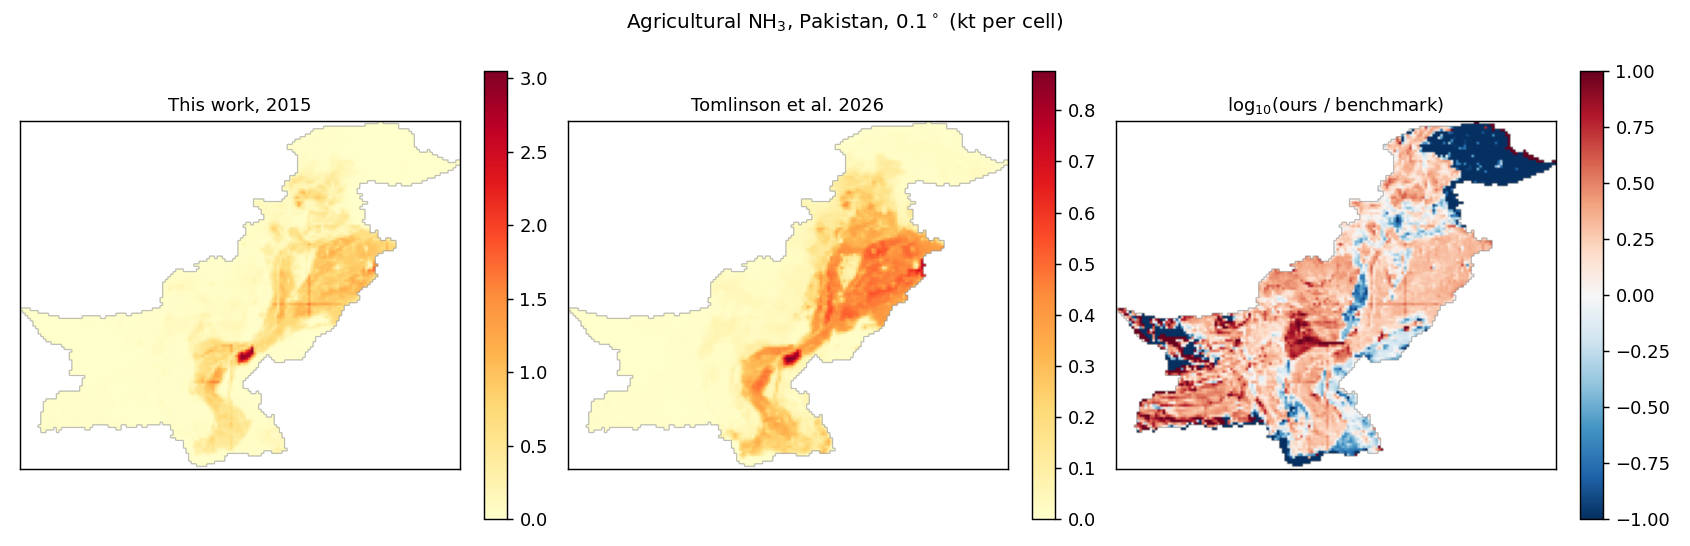
\includegraphics[width=\linewidth]{nh3_spatial_comparison.png}
\caption{Agricultural \NHthree{} emissions over Pakistan in 2015 at
\SI{0.1}{\degree} resolution: this inventory, the independent South Asian benchmark, and their
ratio. The two surfaces show strong spatial agreement but differ in magnitude, with the
largest relative difference over Balochistan's rangelands.
Generated by
\texttt{src/pkinv/eval/spatial\_nh3\_validation.py}.}
\label{fig:nh3spatial}
\end{figure}

\begin{table*}[!htbp]
\centering
\footnotesize
\begin{tabular}{@{}llrrrc@{}}
\toprule
\textbf{Stream} & \textbf{Our spatial input} & \textbf{$r$} & \textbf{Hotspot} & \textbf{Ratio}
& \textbf{Shared?} \\
\midrule
Synthetic fertiliser & WorldCover (upland; rice on MapSPAM) & 0.89 & 72\% & 1.19 & no \\
Livestock (all)      & \GLW{}             & 0.91 & 78\% & 2.47 & \textbf{yes} \\
Residue burning      & FIRMS active fire   & 0.38 & 39\% & 0.21 & no \\
\midrule
All streams          & ---                 & 0.90 & 78\% & 1.76 & partly \\
\bottomrule
\end{tabular}
\caption{Stream-level spatial comparison with the independent South
Asian agricultural \NHthree{} inventory for 2015. The livestock comparison uses a shared
\GLW{} spatial product and is therefore not fully independent. Fertiliser and residue-burning
comparisons use different spatial inputs in the two inventories.
Generated by
\texttt{src/pkinv/eval/spatial\_nh3\_validation.py}.}
\label{tab:spatialstreams}
\end{table*}

\subsection{Comparison of national ammonia estimates}
\label{sec:ap-benchmark}

National \NHthree{} is compared with the South Asian benchmark at the benchmark year of 2015.

Matching the comparison year is important. Agricultural \NHthree{} in the present
reconstruction increases by a factor of \num{1.44} between 2015 and 2024. Comparing the
benchmark's 2015 value directly with the 2024 anchor would combine methodological differences
with nine years of activity growth.

For 2015 this inventory estimates \SI{1862}{}~kt \NHthree{}, compared with \SI{1043}{}~kt in
the South Asian benchmark \citep{sanh2026}. The ratio is \num{1.79}. Comparing the same
benchmark with the 2024 estimate would produce a ratio of \num{2.56}. The 2015 estimate is
\num{1.48} times the corresponding EDGAR v8 value and \num{1.36} times the HTAP v3 value.

The uncertainty intervals provide a stronger diagnostic than the operational factor-of-two
screening range. The South Asian benchmark reports a \SI{95}{\percent} interval of
approximately \SI{764}{}--\SI{1322}{}~kt for Pakistan. The present inventory's 2015 interval
is approximately \SI{1423}{}--\SI{2307}{}~kt. The intervals do not overlap, and the
uncertainty-normalised difference is $z=3.1$. The national difference is therefore larger
than the parametric uncertainty reported by either inventory.

Agreement varies sharply by source. Synthetic-fertiliser \NHthree{} is \num{1.20} times the
benchmark value. Livestock \NHthree{} is approximately \num{2.50} times the benchmark.
Residue-burning \NHthree{} is \num{0.22} times the benchmark value.

The shared nitrogen ledger helps diagnose the livestock difference. After conversion to common
boundaries and an \NHthree{}-N basis, the IPCC and EMEP/EEA livestock chains produce totals
that differ by only a factor of \num{1.24}. However, both remain substantially above the
external benchmark.

This suggests that the difference cannot be attributed solely to choosing the IPCC or
EMEP/EEA loss formulation. Their stage-level estimates remain different, so the formulation
may still contribute, but the shared excreted-nitrogen pool and the assumed
manure-management distribution also require examination.

Country-specific animal masses increase estimated nitrogen excretion. Buffalo are assigned a
typical mass of \SI{380}{\kilogram}, compared with the IPCC default of \SI{295}{\kilogram},
while dairy cattle are assigned \SI{400}{\kilogram} rather than \SI{275}{\kilogram}. The
greenhouse-gas inventory shows a related signal: manure-management emissions are \num{1.38}
times the FAOSTAT value.

The external benchmark does not report an implicit emission factor for buffalo, despite
buffalo being a major component of Pakistan's livestock population. A residual calculation
based on its published national total and the species it reports implies a buffalo factor no
greater than approximately \SI{3.9}{}~kg \NHthree{} per head per year, as set out in
Supplementary Note~S4.

The present reference configuration gives approximately \SI{9.8}{}~kg per buffalo per year,
and the GLEAM~3.0 configuration gives \SI{11.7}{}~kg per head per year. These external
parameterisations therefore imply markedly different assumptions about the treatment of
buffalo manure, particularly the proportion deposited during grazing.

The inferred benchmark factor is not a direct observation. It is calculated as a residual and
also absorbs unresolved contributions from camels. It should therefore be treated as an
indication of where the discrepancy may arise rather than as a definitive attribution.

The available evidence points most strongly to the manure-management distribution, with
animal-mass assumptions and stage-specific loss formulations as additional contributors.
Because the manure-management distribution has not been measured nationally, the livestock
\NHthree{} estimate remains provisional.

The lower residue-burning estimate reflects the wider set of burned crops included in the
external inventory. Its additional \SI{1.4}{}~kt estimate for residues left in fields is too
small to explain the national difference and would increase rather than reduce the gap.

\begin{table*}[!htbp]
\centering
\footnotesize
\begin{tabular}{@{}llrrcrc@{}}
\toprule
& & & \multicolumn{2}{c}{\textbf{Matched year (2015)}}
& \multicolumn{2}{c}{\textbf{Anchor (2024)}} \\
\cmidrule(lr){4-5}\cmidrule(lr){6-7}
\textbf{Scope} & \textbf{Benchmark} & \textbf{Bench.}
& \textbf{Engine} & \textbf{Ratio} & \textbf{Engine} & \textbf{Ratio} \\
\midrule
Synthetic fertiliser & SANH 2026 & 514 & 617 & 1.20 & 737 & 1.43 \\
Livestock (all streams) & SANH 2026 & 496 & 1238 & 2.50$^{\dagger}$ & 1928 & 3.89$^{\dagger}$ \\
Residue burning & SANH 2026 & 32 & 7.0 & 0.22$^{\dagger}$ & 9.2 & 0.29$^{\dagger}$ \\
\midrule
\textbf{National total} & SANH 2026 & 1043 & 1862 & \textbf{1.79} & 2674 & 2.56$^{\dagger}$ \\
\textbf{National total} & EDGAR v8$^{a}$ & 1257 & 1862 & \textbf{1.48} & 2674 & 2.13$^{\dagger}$ \\
\textbf{National total} & HTAP v3$^{a}$ & 1372 & 1862 & \textbf{1.36} & 2674 & 1.95 \\
\bottomrule
\end{tabular}
\caption{Agricultural \NHthree{} compared with external inventories at the
benchmark year of 2015 and, for context, at the 2024 anchor. Matched-year comparisons separate
methodological differences from activity growth. Ratios outside the study's diagnostic
screening range are marked for further investigation.
$^{a}$Implied from the percentage differences
reported by \citet{sanh2026}. One scope mismatch is not corrected for: four
\NHthree{} streams against the study's five sectors.
Generated by \texttt{src/pkinv/sectors/agriculture/air\_pollutants.py}.}
\label{tab:apbench}
\end{table*}

\FloatBarrier
\section{Discussion}
\label{sec:discussion}
Pakistan-specific activity and process boundaries determine the inventory's contribution. Crop, nutrient and census-anchored herd controls support a national reconstruction whose source pathways and geographic support remain inspectable. The common nitrogen ledger permits differences in NH$_3$, NO$_x$ and N$_2$O to be explained by pathway or factor rather than hidden in incompatible accounts.

The retained dry-climate soil factor is consequential and conditional. Irrigated cropland, flooded rice and grazing have different factor applicability, so a national climate label does not resolve every pathway. Aggregate and climate-factor sensitivities show the consequence without fitting to FAOSTAT or national reporting. The same distinction applies to manure-system shares: material closure checks the calculation but does not establish the chosen management distribution.

Independent district crop records evaluate selected spatial patterns. Inventories constructed from the same livestock counts or cropland surfaces do not independently confirm those allocations. Coarse support downscaled to 0.05$^\circ$ retains proxy limitations. Source-matched public HTAP comparisons supplement national reporting and global inventories, with provider and shared-input provenance explicit.

The common core's latest annual year and its detailed reference year have different roles. FY2024--25 uses supportable annual activity; it does not acquire new monthly application dates, herd enumeration or fine-scale source geography automatically. Fitness for use therefore depends on species, emitting process, year and configuration as well as total mass. Atmospheric concentrations, exposure and health effects require additional evidence and are outside this inventory.

\FloatBarrier
% ===========================================================================
\section{Limitations}
\label{sec:limitations}
% ===========================================================================

The estimates are provisional and desk-based. Several limitations follow directly
from the method and should condition interpretation of the results.

\subsection*{Emission factors and tier status}
\begin{enumerate}[leftmargin=1.4em,itemsep=2pt,topsep=2pt]

\item \textbf{Tier~1/2, not Tier~3.} No emission factor is backed by Pakistani
field measurement; the factors are IPCC defaults elevated with country-specific
activity data. The widest uncertainty bands --- rice and soil nitrous oxide ---
reflect this, and it is the principal limitation on inventory confidence.

\item \textbf{Emission-factor context.} With the exception of the empirical
soil-nitrogen anchor, factors originate from IPCC regional defaults; combustion,
manure, and soil processes in Pakistani conditions may differ systematically from
the values underlying those defaults, in either direction.

\item \textbf{The soil direct factor is a deliberate choice.} We use the 2019
dry-climate $\EFone{}=0.005$, which halves managed soils relative to the 2006
aggregate $0.010$ that FAOSTAT retains (Section~\ref{sec:discussion}). We report
the aggregate value as a sensitivity ($\sim$\SI{40}{}~Mt) rather than tune to the
benchmark; the choice is defensible but consequential.

\item \textbf{Rice is modelled as continuously flooded} ($SF_w=1$). The
intermittent and rainfed water-regime scaling factors exist in the factor set but
are not applied, so alternate-wetting-and-drying mitigation is not represented ---
a real simplification on a sizeable, policy-relevant category with a wide
uncertainty band.

\end{enumerate}

\subsection*{Livestock and manure management}
\begin{enumerate}[leftmargin=1.4em,itemsep=2pt,topsep=2pt,resume]

\item \textbf{Manure-management shares are uncertain.} The management-system
split is Tier-2/FAOSTAT-consistent; an alternative South-Asian split would move
manure direct nitrous oxide materially, and the split is not measured for
Pakistan.

\item \textbf{The dung-cake transfer has an observed destination for part of its mass.}
Dung-cake combustion ($\sim$28\% of manure) is removed from this sector's
manure-management balance. The national reference books as household fuel what the
household survey observes, under a fifth of the diverted mass; the remainder is carried
as an unresolved row outside the total with no emission applied, and its candidate fates
are priced rather than chosen. Under national configuration~L, the reference of earlier
releases and now the alternative, all of the diverted mass is RECEIVED by the residential
sector as household fuel, and there the cross-module closure is enforced with an exact
equality, not merely declared (an earlier edition of this item still called the
receiving account out of scope).

\item \textbf{The crop-residue fuel transfer is closed the same way, with a larger
open remainder.} Of \SI{86.14}{}~Mt of dry residue, \SI{9.27}{}~Mt (\SI{122192}{}~TJ) is
diverted to household fuel and received by the residential sector's fuel ledger under the
same exact-equality discipline as dung cake; \SI{20.40}{}~Mt is returned to soil and
\SI{8.37}{}~Mt burned in the field. The \SI{48.10}{}~Mt the ledger cannot place
(\SI{55.8}{\percent} of dry residue---fodder, bedding, industrial use and decay) is
carried as an explicit unresolved row rather than assigned a fate.

\item \textbf{Livestock ammonia is \boldmath$\sim$3$\times$ independent
inventories, and is provisional.} Benchmarking (Section~\ref{sec:ap-benchmark})
shows our synthetic-fertiliser \NHthree{} at 1.20$\times$ and the livestock streams at
2.5$\times$ an independent South Asian inventory \citep{sanh2026}, both compared at the
benchmark's own year. The shared nitrogen ledger
(Section~\ref{sec:results-nledger}) makes the loss formulation a secondary rather than
a primary suspect, but does not eliminate it: the IPCC and EMEP livestock totals agree
to within 1.23$\times$ on a common basis, yet field application and grazing disagree by
factors of 0.66 and 3.5 in opposite directions and partly offset. What it does \emph{not}
do is establish which side is right, because both representations act on the same
excreted-nitrogen pool --- raised by our Tier-2 animal masses, which also leave
manure management at 1.38$\times$ FAOSTAT --- and the benchmark's own livestock
parameters are not fully reproducible (its implicit-emission-factor table omits
buffalo, the dominant species here). We therefore treat the livestock \NHthree{}
estimate and the manure-derived \NtwoO{} that shares its nitrogen as provisional.
Matching the benchmark's \emph{year} removed roughly a third of the apparent gap,
and back-calculating its unpublished buffalo factor
(Section~\ref{sec:ap-benchmark}) points most of the remainder towards the
manure-management split rather than the animal masses or the loss chain. That split
is not measured for Pakistan, and the two external parameterisations that bear on it --- GLEAM 3.0
and this benchmark --- bracket our assumption from opposite sides and disagree
with each other by a factor of three. A national manure-management survey is therefore
the single highest-value data collection identified by this work, and it would move
both the \NHthree{} and the manure \COe{} estimates.

\end{enumerate}

\subsection*{Historical and spatial assumptions}
\begin{enumerate}[leftmargin=1.4em,itemsep=2pt,topsep=2pt,resume]

\item \textbf{Historical source and time-basis transition.} The 1990--2023 series
uses FAOSTAT activity data on a calendar-year basis while 2024 is anchored to the
PBS census on the FY2023--24 fiscal basis; no statistical harmonisation is applied
across this join---neither for the source change nor for the six-month basis
offset---so part of the 2023--2024 change may
reflect either transition rather than true annual activity growth (livestock
species are mapped to a common six-species taxonomy, but levels can differ). Crop
coverage also differs: the historical file carries four crops where the 2024 anchor
carries five, so residue-driven quantities --- the burning greenhouse gases and the
burning air pollutants --- are a few per cent lower before the join than after it.

\item \textbf{Gridded and district maps are allocated surfaces, not
observations.} Within each province the pattern follows a proxy; the
reconciliation invariant guarantees the totals but not the sub-provincial detail.

\item \textbf{District spatial shares are held constant across years.} The
district\,$\times$\,year panel (Section~\ref{sec:results-districtyear}) rescales a
single 2024 spatial pattern to each year's national total, because no multi-year
district activity survey exists. It distributes national growth across space; it
does not detect district-specific shifts in activity.

\end{enumerate}

\subsection*{Validation and uncertainty}
\begin{enumerate}[leftmargin=1.4em,itemsep=2pt,topsep=2pt,resume]

\item \textbf{District validation is uneven.} Only rice and (via wheat area)
managed soils have an independent district record; the livestock, burning and
urea-application categories have none, and their district rankings are therefore unvalidated
against official statistics (Section~\ref{sec:validation-district}).

\item \textbf{Uncertainty treats most components as independent.} Perfect correlation
is modelled among terms that share an emission factor within managed soils --- the
indirect volatilisation and leaching streams, which are separate rows only because
they follow different spatial proxies. All other correlations (shared activity data,
common factor families across categories) are omitted \emph{here}, because this stream
samples component totals rather than parameters, and could widen or narrow the
national interval. The national engine samples a parameter graph instead and carries two
of these couplings explicitly; Supplementary Note~S3 gives their magnitude.

\item \textbf{The reported ammonia interval is parametric, not total.} The
Monte-Carlo band holds the manure-management configuration fixed and varies factors
and activity within it. But that configuration is itself the dominant uncertainty:
across defensible alternatives national \NHthree{} spans \SI{1.67}{}--\SI{2.67}{}~Mt
(Section~\ref{sec:ap-structural}), a wider range than the $\pm$25\% parametric band.
The two are reported separately and should not be combined into a single interval,
because the structural term is a choice between discrete configurations rather than a
distribution.

\item \textbf{Air-pollutant totals are bottom-up, not control totals.} The
air-pollutant layer now carries the same gridded, district, time-series,
Monte-Carlo and key-source treatment as the greenhouse gases, and its spatial
products reconcile to its national totals by construction. But those national
totals are our own bottom-up estimates rather than an audited IPCC control total,
so what the allocation conserves is weaker in provenance than for the GHGs. The
crop-burning factors are IPCC/EMEP/biomass-burning defaults, soil \NOx{} is a small
high-uncertainty term, and none of the layer is field-validated here.

\end{enumerate}

\subsection*{Scope and omitted sources}
\begin{enumerate}[leftmargin=1.4em,itemsep=2pt,topsep=2pt,resume]

\item \textbf{Not-estimated agriculture gaps.} Soil-organic-nitrogen mineralisation
($F_{SOM}$) and liming are marked NE in the completeness table
(\ref{app:completeness}); they require field or national activity data. (Land-sector
gaps --- SOC change, harvested wood products --- are covered in Supplementary
Note~S1.)

\item \textbf{Land sector excluded.} The exploratory Tier-1 land sector is the
least settled part of this work (single-year, contested mangrove sign) and is
reported only in Supplementary Note~S1, excluded from all agricultural results.

\item \textbf{The fire layer is an observation, and observations can be absent.} The
burning surface now rides the reporting period's own detections (the offset window
that stood here---October 2024--May 2025, one season late---was replaced by the
period-matched extraction). The honest cost is sparsity: a district shape carrying
residue-burning panel mass in which VIIRS recorded no fire falls back to a uniform
spread within that shape, declared per event in the grid fallback ledger---where the
dense cropland proxy it replaced could never say a district had no observed fires.

\end{enumerate}



Together these bound the inventory as a transparent, reproducible \emph{backbone}
rather than a measured account: its magnitudes are auditable and its geography
reconciles by construction, but Tier-3 factors, a resolved rice water regime, and
district-level ground data --- each identified above --- are where further effort
would most improve it.

\FloatBarrier
\section{Conclusions}
\label{sec:conclusion}
The maintained agricultural inventory reconstructs Pakistan-specific crop, nutrient and census-anchored livestock activity within the common July 2015--June 2025 core. GHG and air products share their nitrogen and residue flows while preserving different emission equations, chemical mass conventions and geographic supports.

The reference TAN configuration yields \SI{\SectorRefGHG}{\mega\tonne} CO$_2$-equivalent, \SI{\SectorRefNHthree}{\kilo\tonne} NH$_3$ and \SI{\SectorRefNOx}{\kilo\tonne} NO$_2$-equivalent NO$_x$ in FY2023--24. Management and grazing NO$_x$ are included consistently with the volatilised nitrogen used for indirect N$_2$O. The IPCC configuration, regional factor and management cases remain separate structural products.

Shared conditional realisations preserve nitrogen closure and paired historical changes. Missing machinery/dust sources, climate-factor applicability, manure shares, crop-residue fates and allocation uncertainty remain explicit. Direct public HTAP source tables permit traceable matched-year comparisons, while shared inputs limit independence. These products provide source-specific activity and pathway information beyond a clipped global inventory without claiming field validation of every factor or an exposure assessment.

\FloatBarrier

% ---------------------------------------------------------------------------
% Code and data availability
% ---------------------------------------------------------------------------
\section*{Code and data availability}
The full system --- the calculation engine for both the greenhouse-gas and
air-pollutant layers, the shared nitrogen ledger, the gridding and district pipelines,
the versioned data files, the test suite and the outputs reported here --- is
version-controlled in the inventory repository
(\url{https://github.com/PakAirQuality/pakistan-emissions-sectors}). It reproduces from a
single command (\texttt{run\_all.py}) with NO user-supplied input: the FIRMS extraction
is committed and hash-pinned, and the MapSPAM rice raster is held and hash-pinned
beside it (data/gis/manual/RICE\_SOURCES.json) with its cropland-fallback class
deleted from the allow-list, so a checkout without the raster refuses the build
rather than silently substituting (\ref{app:repro}).
DOIs are minted at archival and none exists yet. Activity data derive
from public sources listed in Section~\ref{sec:data}; downloaded caches are
regenerated by the pipeline. The independent ammonia grid used for spatial validation
is redistributed by its authors under an open licence \citep{sanh2026data}.

% ---------------------------------------------------------------------------
% Bibliography
% ---------------------------------------------------------------------------
\bibliographystyle{elsarticle-harv}
\bibliography{../../paper_common/references}

% ---------------------------------------------------------------------------
% Appendix
% ---------------------------------------------------------------------------
\appendix
\renewcommand{\thetable}{\arabic{table}}%
\renewcommand{\thefigure}{\arabic{figure}}%
% ===========================================================================
\section{Reproducibility}
\label{app:repro}
% ===========================================================================

The inventory runs from a documented pipeline (\texttt{python3 run\_all.py}) that
executes the agricultural stages --- national inventory, provincial downscaling,
gridding, district downscaling, time series, Monte-Carlo, key-category, sensitivity,
and uncertainty-input analysis, completeness table, and a consolidated dashboard ---
and writes all tables and figures reported here. The exploratory land sector is an
\emph{optional} module (skipped under \texttt{--quick}; see Supplementary Note~S1)
and feeds none of the agricultural results. The agricultural core runs on the Python
standard library alone; the gridding and figures use an optional geospatial stack.
The shipped surfaces need nothing supplied: the FIRMS extraction and the MapSPAM
rice raster are both committed-or-held and hash-pinned, so ``one command'' means
one command (the default contract is set out below). Every emission factor, parameter, and
activity value is stored in a versioned data file, and a suite of more than 240 unit
tests checks the IPCC worked-example calculations, exact reconciliation at each scale
(national, provincial, gridded, district, and the district\,$\times$\,year panel),
emission-factor traceability, and the key-category, sensitivity, uncertainty, and
completeness outputs. The suite also covers the air-pollutant engine and its shared
nitrogen ledger --- ledger closure at every stage, the separation of the pre-field and
post-application volatilisation fractions, conservation between the \NHthree{}-N and
\NHthree{}+\NOx{} bases, the province and grid allocation of every pollutant, the
matched-year and spatial benchmarks, and the structural manure-management scenarios ---
together with a consistency check that every headline number and figure in this
manuscript still matches the output file it was generated from.

\paragraph{Code and data availability.} The full source code, data files and tests are
version-controlled; DOIs are minted at archival (none exists yet, and no identifier is
printed before it resolves), and the archived release corresponding to any submitted
version will let reviewers run the same code that produced these numbers. The archive contains the calculation engine for both
layers, the shared nitrogen ledger (\texttt{outputs/n\_ledger\_2024.csv}, every stage-flow
row as kilograms of nitrogen and as a share of what was excreted) and its diagnostic runs
(\texttt{outputs/n\_ledger\_stage\_comparison.csv}, the IPCC and EMEP ammonia-nitrogen
factors set against each other stage by stage), the versioned emission-factor
and activity files, the gridded (GeoTIFF, EPSG:4326) and district (CSV) products, the
1990--2024 time series, the uncertainty and benchmark outputs---including
\texttt{outputs/air\_\allowbreak uncertainty\_\allowbreak montecarlo.csv}, the
per-pollutant intervals with the Approach~1 comparison beside them---and the test suite; units,
coordinate reference system and time coverage are recorded with each product, and a run
manifest records the exact inputs behind the tables reported here. Reproduction: install the (optional) geospatial stack and
run \texttt{python3 run\_all.py}. The shipped surfaces reproduce as-is with no
user-supplied input; the contract is stated in full in \ref{app:data}. Expected outputs are the CSV tables and PNG figures
reproduced here (written under \texttt{outputs/}). The deposited capsule carries its own
single command, \texttt{sh capsule/run\_tests.sh}, which reruns the agriculture suite in a
fresh interpreter with nothing installed; in the full repository
\texttt{python3 -m pytest tests} runs the
test suite, as does \texttt{python3 -m unittest discover tests}, which is what continuous
integration uses. On the released commit both pass in full; on any other commit the
release-integrity tests fail by design: they compare the
committed release artefacts---manifest, cover, checksums, PDFs---against the working tree,
and they can only pass on the exact commit the artefacts were cut from. They are not a failed
reproduction, and a reader who sees them should not read them as one. The code is released under the MIT licence and the derived data under
CC-BY-4.0; third-party inputs retain their original licences.

\section{Data acquisition}
\label{app:data}

THE REPRODUCTION CONTRACT, stated once. Livestock density (\GLW{}, 2020) is retrieved
directly from the FAO open cloud store. The FIRMS VIIRS extraction is \emph{committed}
and hash-pinned in \texttt{data/gis/manual/}, so no access key is needed to reproduce
(a key is needed only to RE-FETCH, which would create a new extraction). MapSPAM~2020
is \emph{held} (V2r2, hash-pinned in \texttt{RICE\_SOURCES.json}) and its former
cropland-fallback class is deleted from the allow-list, so a checkout missing the
raster refuses the build rather than silently substituting. The DEFAULT reproducible
surface is therefore: MapSPAM for rice, frozen FIRMS for burning, and nothing to
supply. Re-fetching FIRMS or swapping the rice surface (the own-year GCD-Rice 2023
classification ships as the priced alternative) changes the surface and is an
\emph{upgrade}: it creates a new configuration and a new manifest, and its outputs
are not the ones reported here. The
pipeline auto-detects supplied files and logs which proxy each category used.

\section{IPCC common reporting table}
\label{app:crt}

Table~\ref{tab:crt} gives a Common-Reporting-Table view of the agriculture sector
for the base year (1990) and the latest year (2024): the underlying activity data,
the implied emission factor, and the resulting \COe{}. The principal emission and
carbon factors themselves are listed in the body (Table~\ref{tab:ef-full}).

\begin{table}[!htbp]
\centering
\footnotesize
\setlength{\tabcolsep}{3pt}
\begin{tabular}{@{}p{0.22\linewidth}lp{0.30\linewidth}rr@{}}
\toprule
\textbf{Code / category} & \textbf{Gas} & \textbf{Activity (2024)}
& \textbf{1990} & \textbf{2024} \\
\midrule
3.A Enteric ferment. & \CHfour{} & 245.52 M ruminant head & 54.5 & 151.7 \\
3.B Manure mgmt.\ & \CHfour{} & 245.52 M ruminant head$^{a}$ & 4.3 & 13.2 \\
3.B Manure mgmt.\ & \NtwoO{} & 7.78 M t N excreted$^{a}$ & 2.4 & 8.0 \\
3.C Rice cultivation & \CHfour{} & 3.64 M ha paddy & 9.6 & 16.5 \\
3.D Managed soils & \NtwoO{} & F$_{SN}$ 3.78, F$_{ON}$ 2.34, F$_{PRP}$ 3.18, F$_{CR}$ 0.21 M t N$^{d}$ & 10.3 & 28.5 \\
3.F Field burning & \CHfour{},\NtwoO{} & 7.11 M t d.m.\ combusted$^{c}$ & 0.3 & 0.7 \\
3.H Urea application & \COtwo{} & 6.58 M t urea$^{b}$ & 1.9 & 4.8 \\
\midrule
\textbf{Agriculture total} & & & \textbf{83.2} & \textbf{223.5} \\
\bottomrule
\end{tabular}
\caption{IPCC CRT-style summary by category and gas, 1990 and 2024 (\COe{} in Mt,
AR5). $^{a}$Manure CH\textsubscript{4} is driven by the ruminant herd and its
N\textsubscript{2}O by the nitrogen excreted by that herd; both are independent of
the synthetic-fertiliser series. Poultry adds to the head-count but little emission. $^{b}$Urea mass is NFDC's printed national
offtake for the fiscal year; earlier years, which have no published product split, keep the
derivation from the national synthetic-N series, and each year states which it used.
$^{c}$The residue activity is dry matter actually
\emph{combusted}: production $\times$ residue ratio $\times$ burned fraction gives
\SI{8.4}{}~Mt of dry matter reaching the fire, of which the combustion factor
$C_f=0.85$ leaves \SI{7.1}{}~Mt burnt. Emission factors are applied to the latter. The full
destination accounting is published in
\texttt{outputs/agriculture\_crop\_residue\_ledger\_2024.csv}.
Liming (3.G): not estimated, assumed negligible on
Pakistan's alkaline, calcareous soils pending national lime-use data.
$^{d}$The four nitrogen inputs of Eq.~11.1, from the shared ledger: synthetic
fertiliser, applied organic manure, pasture deposition and crop residue. They are not
summed here because the pasture term carries its own factor (EF$_{3\mathrm{PRP}}$).}
\label{tab:crt}
\end{table}

\section{Completeness and QA/QC}
\label{app:completeness}

Table~\ref{tab:completeness} gives the notation-key coverage of the agriculture
categories. All major agriculture source categories are represented, with the
not-estimated (NE) gaps shown explicitly: soil-organic nitrogen mineralisation
($F_{SOM}$), which requires field data; and liming, set to NE (assumed negligible on
Pakistan's alkaline, calcareous soils pending national lime-use data) rather than
assumed not to occur. Dung-cake combustion is the one cross-sector transfer to
Energy. Land-sector completeness (forest, cropland/grassland SOC, wetlands,
harvested wood products) is documented in Supplementary Note~S1. Air-pollutant
co-emissions (\NHthree{}, \NOx{}, PM$_{2.5}$, CO, NMVOC, BC) are estimated for the
relevant categories in Section~\ref{sec:airpollutants} and reported in native mass,
outside this \COe{} completeness table; agricultural SO$_2$ is estimated but small
($\sim$2.6~kt, from residue burning only). Quality control is automated (source
traceability, unit checks, exact reconciliation, benchmark bands); quality
assurance is the independent FAOSTAT and EDGAR comparison; and any method or factor
change --- such as the harmonisation of the volatilisation factor $EF_4$ to the
dry-climate value across the manure and soils terms --- triggers a full
1990--2024 recalculation to preserve time-series consistency.

\begin{table}[!htbp]
\centering
\footnotesize
\begin{tabular}{@{}llc@{}}
\toprule
\textbf{Category} & \textbf{Gas} & \textbf{Key} \\
\midrule
3.A Enteric fermentation        & \CHfour{}          & E \\
3.B Manure management           & \CHfour{}, \NtwoO{} & E \\
3.C Rice cultivation            & \CHfour{}          & E \\
3.D Agricultural soils          & \NtwoO{}           & E \\
\quad SOC mineralisation ($F_{SOM}$) & \NtwoO{}      & NE \\
3.E Savanna burning             & ---                & NO \\
3.F Field burning of residues   & \CHfour{}, \NtwoO{} & E \\
3.G Liming                      & \COtwo{}           & NE \\
3.H Urea application            & \COtwo{}           & E \\
Dung-cake combustion            & multi              & IE \\
\bottomrule
\end{tabular}
\caption{Completeness and notation keys for the agriculture sector (IPCC Vol.~1
Ch.~8). E~estimated, NE~not estimated, NO~not occurring, IE~included elsewhere
(Energy). Land-sector categories are in Supplementary Note~S1.}
\label{tab:completeness}
\end{table}

\section{Uncertainty inputs}
\label{app:unc}

The uncertainty analysis (Section~\ref{sec:methods}) is reproducible from the inputs
below. Each category's combined uncertainty is a two-stage quadrature: every emission
component combines an activity-data and an emission-factor uncertainty (Eq.~3.1), and
the components are aggregated to the category (Eq.~3.2). The full underlying-input
table --- per component, the activity-data uncertainty, the factor uncertainty, their
sources, and which inputs are shared across categories --- is given in Supplementary
Note~S3; the factor uncertainties also appear as the $\pm$\% column of
Table~\ref{tab:ef-full}. Table~\ref{tab:unc} gives the resulting per-category
distribution used by the ANALYTIC comparison alone---the Monte-Carlo samples the engine's
components, not these fitted category distributions: the point estimate $E_c$, the combined
95\% half-width, and the mean-preserving lognormal parameters
$\sigma_{\ln}=(\text{half-width}/100)/1.96$ and
$\mu_{\ln}=\ln E_c-\sigma_{\ln}^2/2$. Correlation is modelled in one specific place and
not elsewhere, and the distinction matters: components that are separate rows only
because they follow different spatial proxies --- the managed-soils indirect
volatilisation and leaching streams --- share a single emission factor ($EF_4$ and
$EF_5$ respectively), so they are treated as perfectly correlated, summed linearly
before the quadrature step and given one shared deviate per group in the
Monte-Carlo. Treating them as independent would shrink the reported band purely
because the rows were cut more finely. All other within- and cross-category
correlations (shared activity data, common factor families across categories) are
\emph{not} modelled as shared deviates \emph{in this sector-scoped stream}, which samples
component totals; the national run's parameter graph does carry two of them, and
Supplementary Note~S3 reports their effect. Approach~1 combines these analytically; the
Monte-Carlo samples the \emph{components} themselves---each row drawn
mean-preserving lognormal at its declared width, with the correlated soils groups
receiving one shared deviate per draw---and the category and sector totals are the
sums of those sampled rows in every realisation.

\begin{table}[!htbp]
\centering
\footnotesize
\begin{tabular}{@{}lcccc@{}}
\toprule
\textbf{Category} & \textbf{$E_c$ (Mt)} & \textbf{$\pm$\% (95\%)} & \textbf{$\mu_{\ln}$} & \textbf{$\sigma_{\ln}$} \\
\midrule
Enteric fermentation & 151.7 & 25.4 &  5.013 & 0.129 \\
Manure management    &  21.2 & 32.9 &  3.042 & 0.167 \\
Managed soils        &  28.5 & 47.1 &  3.323 & 0.237 \\
Rice cultivation     &  16.6 & 60.9 &  2.760 & 0.304 \\
Field burning        &   0.7 & 44.9 & $-0.426$ & 0.226 \\
Urea application     &   4.8 & 11.2 &  1.571 & 0.057 \\
\midrule
\textbf{Total}       & \textbf{223.4} & \textbf{19.1} & --- & --- \\
\bottomrule
\end{tabular}
\caption{Derived per-category uncertainty parameters. $\mu_{\ln},\sigma_{\ln}$ are
the mean-preserving lognormal parameters implied by each category's 95\% half-width, and
they describe an ANALYTIC comparison, not the simulation: the Monte-Carlo samples the
engine's \emph{components} (with shared deviates inside declared correlation groups) and
obtains each category as the sum of its sampled rows. The national total is likewise a
sum, never a sampled input distribution, so no $\mu_{\ln}/
\sigma_{\ln}$ is given for it. Underlying activity/factor inputs and sources are in
Supplementary Note~S3. Generated by \texttt{src/pkinv/eval/uncertainty\_inputs.py}.}
\label{tab:unc}
\end{table}


\end{document}
